\documentclass[12pt]{article}
\usepackage[margin=1in]{geometry}
\usepackage{graphicx}
\usepackage{amsmath,amssymb,bm}
\usepackage{booktabs}
\usepackage[table]{xcolor}
\usepackage{array}
\usepackage{multirow}
\usepackage{setspace}
\usepackage{enumitem}
\usepackage{rotating}
\usepackage{tikz}
\usetikzlibrary{positioning,arrows.meta}
\usepackage{hyperref} % load hyperref BEFORE biblatex
\usepackage[backend=biber,style=numeric,autocite=superscript]{biblatex}
\addbibresource{bibliography.bib}
\addbibresource{new_references.bib}

\onehalfspacing

\title{Generalized Machine Learning for Fast Calibration of Agent-Based Epidemic Models}
\date{}

\begin{document}
\maketitle

% =============================================================================
\begin{abstract}
\noindent\textbf{Background.}
Agent-based models (ABMs) describe how an epidemic spreads through the contacts between
individuals, and they are increasingly used to support public health decisions. Before an ABM can
be used, its parameters have to be calibrated to the observed data. Standard calibration methods,
such as approximate Bayesian computation (ABC) and numerical optimization, run the model thousands
of times for every data set, which makes them slow and requires many choices from the user.

\noindent\textbf{Methods.}
We present DeepIMC (Deep Inverse Mapping Calibration), a neural network that learns the inverse
mapping from an epidemic curve to the quantities that produced it. DeepIMC is trained once, on
1,000,000 epidemics simulated with agent-based SEIR and SIR models, and then calibrates a new
curve in a single pass of the network. It reads a window of daily new infections of any length
between 15 and 365 days, taken from any part of an epidemic, and returns the basic reproduction
number $R_0$ with a 95\% range, the transmission probability and contact rate, and the state of
the epidemic on the first day of the window. We compared DeepIMC with four standard calibration
methods used with their default settings (ABC-MCMC, ABC-SMC, differential evolution and
Nelder--Mead) on 10,000 simulated test epidemics, measuring both the accuracy of the estimated
parameters and how well each method's estimates reproduce the epidemic curves, and on five real
datasets chosen because their counts follow new infections closely. All computing times were
measured on CPUs.

\noindent\textbf{Results.}
On 10,000 simulated test windows of 15 to 365 days, DeepIMC estimated $R_0$ with a mean absolute
error of 0.19, about three times smaller than the best comparison method (0.61 for SEIR and 0.49 for SIR),
and it was more accurate than that method on 74--83\% of the windows and in every group of window length
and position. Its 95\% ranges contained the true $R_0$ in 96--97\% of the windows while being three to four
times narrower than those of the ABC methods. No method could separate the transmission probability from
the contact rate, because only their product shapes the curve. Curves regenerated from DeepIMC's
estimates matched the observed new infections as closely as the best comparison method, and more
closely when DeepIMC's draws were weighted by the data, and recovered the unobserved number of infectious
people with half its error and 98--99\% coverage; the weighted interval
score, which combines accuracy and coverage, and the cumulative incidence gave the same picture. Starting
from DeepIMC's estimated state rather than from a naive one, or from one fitted by the renewal equation,
was essential. On real data, DeepIMC fitted short windows and the influenza and Ebola series almost as
closely as the best comparison method, and was weaker on long windows and on outbreaks brought under
control. Weighting DeepIMC's parameter draws by how well they reproduce the data, without retraining,
brought it closer to the data on four of the five datasets, and the same step flags the windows that the
model cannot reproduce. On one CPU core, DeepIMC calibrated a window
in 0.08 to 0.15 seconds, against 3 to 588 seconds for the comparison methods.

\noindent\textbf{Conclusions.}
DeepIMC calibrates agent-based epidemic models accurately, reproduces the epidemic they describe,
and does so in a fraction of a second, with no settings to choose. Its advantage on real data
depends on how closely the data resemble the simulations it was trained on. The method, the trained
models and the comparison methods are available in the open-source R package
\texttt{epiworldRcalibrate}.
\end{abstract}

\noindent\textbf{Keywords:}
agent-based models; epidemic modeling; model calibration; machine learning; neural networks;
approximate Bayesian computation; simulation-based inference

% =============================================================================
\section{Introduction}

Agent-based models (ABMs) simulate an epidemic one person at a time: each agent has a state
(susceptible, exposed, infectious or recovered), meets other agents, and may transmit or acquire
an infection. Because they represent individuals and their contacts explicitly, ABMs can describe
heterogeneous populations, interventions that target particular groups, and the randomness of
small outbreaks, which simpler compartmental models cannot. For these reasons they are widely used
to explore the course of epidemics and the effect of public health measures
\autocite{railsbackAgentbasedIndividualbasedModeling2019}.

An ABM is only useful once it is \emph{calibrated}, that is, once its parameters have been chosen
so that the model reproduces the observed data. For an epidemic model, the most important of these
parameters describe transmission: how many contacts an infectious person has per day, and how
likely each contact is to transmit the infection. Calibrating an ABM is computationally demanding.
The model has no likelihood that can be written down, so calibration methods must run the model
many times and compare its output with the data. Approximate Bayesian computation (ABC) and
numerical optimization methods typically need thousands of model runs for each data set, and the
whole procedure has to be repeated whenever new data arrive, for every location and every time
period of interest. During an outbreak, when estimates are needed quickly and repeatedly, this cost
limits how ABMs can be used.

A second difficulty is that standard calibration methods require many decisions from the user:
the prior ranges of the parameters, how to compare simulated and observed curves (the whole curve
or a set of summary statistics), tolerances, the number of iterations or particles, and the
starting values. These choices affect the results, and making them well requires expertise in
both the model and the calibration method.

Machine learning offers a different route. Rather than searching the parameter space for every new
data set, a neural network can be trained once, on simulations from the model, to map the observed
data directly to the parameters that generated them. This idea, often called \emph{amortized} or
\emph{simulation-based} inference \autocite{cranmer2020frontier,radev2022bayesflow}, moves the
computational cost to a one-time training phase; afterwards, calibrating a new data set takes a
single pass of the network. Most applications of machine learning to ABM calibration have instead
built surrogate models, which approximate the mapping from parameters to model outputs and still
require a search over parameters for every data set
\autocite{Angione2022-surrogate,lamperti2017agentbasedmodelcalibrationusing}.

In this paper we develop and evaluate DeepIMC (Deep Inverse Mapping Calibration), a neural network
that calibrates agent-based SEIR and SIR epidemic models from the \textbf{epiworldR} package
\autocite{meyerEpiworldRFastAgentBased2023}. DeepIMC is designed for the data available in
practice. Analysts rarely observe a complete epidemic from its first case: they work with the last
weeks or months of data, which may start in the middle of a wave. DeepIMC therefore reads a window
of daily new infections of any length between 15 and 365 days, from any part of an epidemic, and
estimates, besides the parameters, the state of the epidemic on the first day of the window: how
many people are exposed, infectious and recovered. This state is what is needed to simulate the
epidemic forward.

Our contributions are the following.
\begin{enumerate}[leftmargin=*]
\item We describe DeepIMC, which estimates the basic reproduction number $R_0$, the transmission
probability, the contact rate and the current state of an agent-based epidemic from a window of
daily new infections, together with a 95\% range for $R_0$.
\item We compare DeepIMC with four standard calibration methods---ABC-MCMC, ABC-SMC, differential
evolution and Nelder--Mead---used as a practitioner would use them, on 10,000 simulated test
epidemics. We evaluate not only the accuracy of the estimated parameters but also how well each
method's estimates reproduce the epidemic: the observed curve, the number of people currently
infectious (which no method observes), and the following two weeks.
\item We evaluate all methods on five real datasets, which we selected by checking what each
dataset counts and whether those counts follow new infections closely enough to be modelled.
\item We compare the computing time of all methods on CPUs, separating the one-time cost of
training DeepIMC from the cost of calibrating a new data set.
\item We provide the method, the trained models, the comparison methods and the evaluation tools in
the open-source R package \texttt{epiworldRcalibrate}.
\end{enumerate}

The rest of the paper is organized as follows. Section~\ref{sec:background} reviews calibration
methods for agent-based models. Section~\ref{sec:methods} describes the models, DeepIMC, the
comparison methods and the evaluation. Section~\ref{sec:results} presents the results on simulated
and real data and the computing times, and Section~\ref{sec:discussion} discusses what they mean
for the use of agent-based models in practice.

% =============================================================================
\section{Calibrating agent-based models}\label{sec:background}

\paragraph{Agent-based models.} An agent-based model consists of agents, the rules by which they
interact (the topology of their contacts), and their environment
\autocite{railsbackAgentbasedIndividualbasedModeling2019}. In an epidemic ABM, each agent is in one
disease state at a time, and the transitions between states happen at random according to the
model's parameters and the agent's contacts. The behaviour of the whole population---the epidemic
curve---emerges from these individual events. Because the model is stochastic, running it twice
with the same parameters gives two different epidemics.

\paragraph{The calibration problem.} Calibration seeks the parameter values for which the model's
output resembles the observed data. For an ABM the probability of the observed data given the
parameters (the likelihood) cannot be computed, so calibration methods compare simulated and
observed data directly. Strategies include approximate Bayesian computation
\autocite{toniApproximateBayesianComputation2008,gozzi2022preliminary}, simulated minimum distance
and other optimization methods \autocite{platt2020comparison}, and surrogate models
\autocite{lampertiAgentbasedModelCalibration2018,jalalBayCANNStreamliningBayesian2021,zhang2020validation}.

\paragraph{Approximate Bayesian computation.} ABC approximates the posterior distribution of the
parameters by keeping parameter values whose simulated data are close to the observed data. The
data are usually reduced to summary statistics, and closeness is measured by a distance between the
observed and simulated statistics \autocite{beaumont2002approximate}. In its simplest form, ABC
draws parameters from the prior and accepts those within a tolerance; this is very inefficient when
the prior is wide. ABC-MCMC \autocite{marjoramMarkovChainMonte2003} explores the parameter space
with a Markov chain, proposing small moves from the current value, and ABC-SMC
\autocite{toniApproximateBayesianComputation2008,beaumont2009adaptive} moves a population of
particles through a sequence of decreasing tolerances. Both return samples from an approximate
posterior, and both need thousands of model runs per data set.

\paragraph{Optimization.} Optimization methods search for the single parameter value whose simulated
output is closest to the data. Differential evolution \autocite{storn1997differential} evolves a
population of candidate solutions by combining them, and is robust to local minima; the
Nelder--Mead simplex method \autocite{nelder1965simplex} moves a small set of points downhill and
needs far fewer model runs, but can stop early when the objective is flat or noisy, as it is for a
stochastic model. Optimization gives a point estimate, without a measure of uncertainty.

\paragraph{Surrogates and amortized inference.} A surrogate (or emulator) is a fast statistical
model of the mapping from parameters to model output, fitted to a set of model runs; it speeds up
each evaluation, but calibration still searches the parameter space for every data set.
\emph{Amortized} inference instead learns the inverse mapping, from data to parameters, once, from
simulations \autocite{cranmer2020frontier,radev2022bayesflow}. After training, calibrating a new data
set costs one evaluation of the learned mapping. DeepIMC follows this approach, with a recurrent
neural network that reads the epidemic curve day by day.

% =============================================================================
\section{Methods}\label{sec:methods}

\subsection{The agent-based models}\label{sec:models}

We consider the two connected (homogeneous mixing) models of \textbf{epiworldR}:
\texttt{ModelSEIRCONN}, in which agents are susceptible, exposed, infectious or recovered, and
\texttt{ModelSIRCONN}, without the exposed state. Each day, every infectious agent meets on average
$c_{rate}$ randomly chosen agents (the \emph{contact rate}), and each meeting with a susceptible
agent transmits the infection with probability $p_{tran}$ (the \emph{transmission probability}).
In the SEIR model, an infected agent first becomes exposed and moves to the infectious state with
daily probability $1/\text{incub}$, so that incub is the mean latent period in days. Infectious
agents recover with daily probability $p_{recov}$, so that $1/p_{recov}$ is the mean infectious
period. The basic reproduction number, the mean number of people infected by one infectious person
in a fully susceptible population, is
\begin{equation}\label{eq:R0}
R_0 = \frac{p_{tran}\, c_{rate}}{p_{recov}}.
\end{equation}

\paragraph{What a curve can reveal.} In these models the chance that a susceptible agent is infected
on a given day depends on $p_{tran}$ and $c_{rate}$ only through their product, $p_{tran} \times
c_{rate}$, the daily transmission rate. Two pairs with the same product produce epidemics with the
same distribution: for example, $p_{tran} = 0.071$ with $c_{rate} = 5$, and $p_{tran} = 0.024$ with
$c_{rate} = 15$, give the same epidemic. A curve of daily new infections can therefore reveal $R_0$
(given the known recovery rate), but not how it splits into $p_{tran}$ and $c_{rate}$. We report the
estimates of all three parameters, and compare the errors in $p_{tran}$ and $c_{rate}$ with those of
a guess that knows $R_0$ exactly but not the split.

\subsection{The calibration problem}\label{sec:problem}

\paragraph{The data.} The observed data are a \emph{window}: the daily counts of new infectious
people (transitions from exposed to infectious in the SEIR model, from susceptible to infectious in
the SIR model) over $L$ consecutive days, with $30 \le L \le 365$. The window may come from the
beginning, the middle or the end of an epidemic.

\paragraph{The known values.} As is common in applied epidemic modelling, we assume that some
quantities are known or can be taken from other studies: the population size $N$, the recovery rate
$p_{recov}$ and, for the SEIR model, the latent period incub.

\paragraph{The unknowns.} DeepIMC estimates $R_0$, $p_{tran}$ and $c_{rate}$, and the state of the
epidemic on the first day of the window: the shares of the population exposed (SEIR), infectious and
recovered. The state matters as much as the parameters: a window from the middle of an epidemic
starts with many people already infected or immune, and the same parameters lead to very different
futures depending on that state.

\subsection{Training data}\label{sec:training-data}

For each model we simulated 1,000,000 epidemics of 365 days. The parameters of each epidemic were
drawn independently from the distributions in Table~\ref{tab:priors}, chosen to cover a wide range
of respiratory infections: $R_0$ between 0.8 and 5, recovery rates between 0.071 and 0.25 (an
infectious period of 4 to 14 days), latent periods of 1 to 21 days, and populations of 5,000 to
10,000. Each epidemic started with a share of the population exposed (SEIR) or infectious (SIR)
drawn on the logarithmic scale between 0.1\% and 40\%, so that both small outbreaks and epidemics
already well under way are represented. For every day we stored the number of new infectious people
and the shares of the population in each state. Epidemics with fewer than 20 cases in total were
discarded (0.1\% for SEIR and 0.2\% for SIR). These data are noise-free: every new infection is
counted.

\begin{table}[htbp]
\centering
\caption{Distributions used to simulate the training, calibration and test epidemics.}
\label{tab:priors}
\small
\begin{tabular}{lll}
\toprule
Quantity & SEIR & SIR \\
\midrule
Population size $N$ (known) & uniform, 5,000 to 10,000 & same \\
Recovery rate $p_{recov}$ (known) & uniform, 0.071 to 0.25 & same \\
Latent period incub (days, known) & uniform, 1 to 21 & -- \\
Basic reproduction number $R_0$ & uniform, 0.8 to 5 & same \\
Contact rate $c_{rate}$ & uniform, 5 to 15 & uniform, 1 to 5 \\
Transmission probability $p_{tran}$ & $R_0\,p_{recov}/c_{rate}$ & same (at most 1) \\
Initial share exposed (SEIR) or infectious (SIR) & log-uniform, 0.001 to 0.4 & same \\
Days simulated & 365 & 365 \\
\bottomrule
\end{tabular}
\end{table}

\paragraph{Windows.} The network is trained on windows cut from these epidemics, not on whole
epidemics. Every training batch cuts one window from each epidemic in the batch. All windows of a
batch share one length, drawn uniformly between 15 and 365 days, and each window starts at a random
day within the \emph{informative} part of its epidemic: the days before the first run of seven days
without new infections. Later days carry no information and are never observed in practice. A new set
of windows is drawn every epoch, so the network sees each epidemic through many different windows.

\subsection{The network}\label{sec:network}

\paragraph{Why a recurrent network.} A window is a sequence of daily counts whose length varies from
one data set to the next. A long short-term memory (LSTM) network \autocite{hochreiter1997long} reads
such a sequence one day at a time and keeps a summary of what it has seen, so the same network can
read windows of any length. We use a \emph{bidirectional} LSTM, which reads the window both forwards
and backwards, so that the summary of every day uses the whole window; this helps the network
recognise whether the window covers the growth, the peak or the decline of an epidemic.

\paragraph{Inputs.} The daily counts are transformed as $\log(1 + x_t)/\log(1 + 10{,}000)$, which puts
small and large epidemics on a comparable scale. The known values ($N$, $p_{recov}$ and, for SEIR,
incub) are scaled to the interval from 0 to 1.

\paragraph{Architecture.} Figure~\ref{fig:architecture} shows the network. The final states of the forward and backward LSTM are joined with the known
values and passed through a dense layer of 64 units and an output layer with one unit per target.
The SEIR network has three LSTM layers of 128 units in each direction; the SIR network, two layers of
64 units. These settings were chosen by a hyperparameter search (below).

\begin{figure}[htbp]
\centering
\resizebox{\textwidth}{!}{% DeepIMC network (the shipped SEIR and SIR models). Needs tikz with the positioning and arrows.meta
% libraries. \input inside a figure environment.
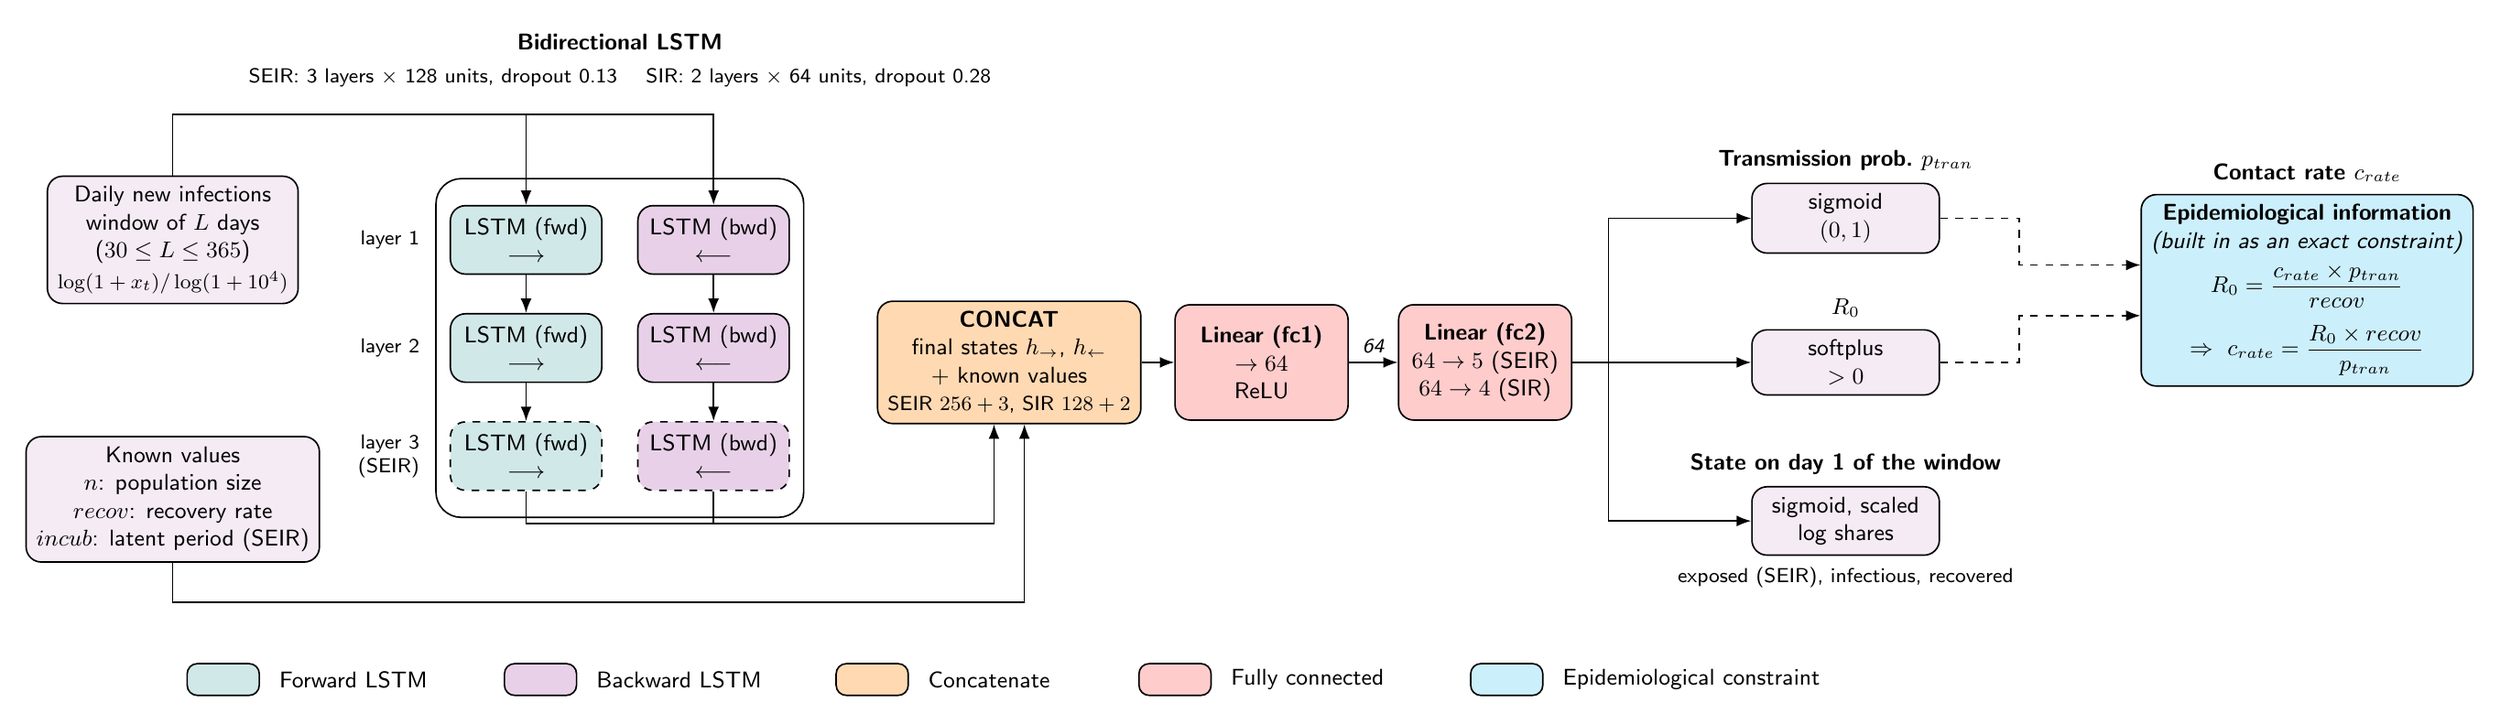
\begin{tikzpicture}[
  font=\sffamily\small, >=Latex, line width=0.6pt,
  box/.style={draw, rounded corners=6pt, align=center, inner sep=4pt},
  inp/.style={box, fill=violet!8, minimum width=3.2cm},
  fwd/.style={box, fill=teal!18, minimum width=2.1cm, minimum height=0.95cm},
  bwd/.style={box, fill=violet!18, minimum width=2.1cm, minimum height=0.95cm},
  catbox/.style={box, fill=orange!30, minimum width=3.6cm, minimum height=1.6cm},
  fcbox/.style={box, fill=red!20, minimum width=2.4cm, minimum height=1.6cm},
  outbox/.style={box, fill=violet!8, minimum width=2.6cm},
  der/.style={box, fill=cyan!20, minimum width=3.0cm},
  lab/.style={font=\sffamily\bfseries\small}
]
% Inputs
\node[inp] (inc) at (0, 2.6) {Daily new infections\\ window of $L$ days\\ ($30 \le L \le 365$)\\[1pt] {\footnotesize $\log(1+x_t)/\log(1+10^4)$}};
\node[inp] (known) at (0, -1.0) {Known values\\ $n$: population size\\ $recov$: recovery rate\\ $incub$: latent period (SEIR)};

% BiLSTM stack
\node[fwd] (f1) at (4.9, 2.6) {LSTM (fwd)\\ $\longrightarrow$};
\node[bwd] (b1) at (7.5, 2.6) {LSTM (bwd)\\ $\longleftarrow$};
\node[fwd] (f2) at (4.9, 1.1) {LSTM (fwd)\\ $\longrightarrow$};
\node[bwd] (b2) at (7.5, 1.1) {LSTM (bwd)\\ $\longleftarrow$};
\node[fwd, dashed] (f3) at (4.9, -0.4) {LSTM (fwd)\\ $\longrightarrow$};
\node[bwd, dashed] (b3) at (7.5, -0.4) {LSTM (bwd)\\ $\longleftarrow$};
\node[font=\sffamily\footnotesize, anchor=east] at (3.55, 2.6) {layer 1};
\node[font=\sffamily\footnotesize, anchor=east] at (3.55, 1.1) {layer 2};
\node[font=\sffamily\footnotesize, anchor=east, align=right] at (3.55, -0.4) {layer 3\\ (SEIR)};
\draw[rounded corners=10pt] (3.65, -1.25) rectangle (8.75, 3.45);
\node[lab, align=center] at (6.2, 5.35) {Bidirectional LSTM};
\node[font=\sffamily\footnotesize, align=center] at (6.2, 4.85) {SEIR: 3 layers $\times$ 128 units, dropout 0.13 \quad SIR: 2 layers $\times$ 64 units, dropout 0.28};
\foreach \a/\b in {f1/f2, f2/f3, b1/b2, b2/b3} \draw[->] (\a) -- (\b);

% Input routing (both directions read the whole window)
\draw[->] (inc.north) -- ++(0, 0.85) -| (f1.north);
\draw[->] (inc.north) ++(0, 0.85) -| (b1.north);

% Final states and known values to the concatenation
\node[catbox] (cat) at (11.6, 0.9) {\textbf{CONCAT}\\ final states $h_{\rightarrow}$, $h_{\leftarrow}$\\ + known values\\ {\footnotesize SEIR $256+3$, SIR $128+2$}};
\draw[->] (f3.south) -- ++(0, -0.45) -| ([xshift=-6pt]cat.south);
\draw (b3.south) -- ++(0, -0.45);
\draw[->] (known.south) -- ++(0, -0.55) -| ([xshift=6pt]cat.south);

% Dense layers
\node[fcbox] (fc1) at (15.1, 0.9) {\textbf{Linear (fc1)}\\ $\to 64$\\ ReLU};
\node[fcbox] (fc2) at (18.2, 0.9) {\textbf{Linear (fc2)}\\ $64 \to 5$ (SEIR)\\ $64 \to 4$ (SIR)};
\draw[->] (cat) -- (fc1);
\draw[->] (fc1) -- node[above, font=\sffamily\footnotesize\itshape] {64} (fc2);

% Outputs
\node[outbox] (o1) at (23.2, 2.9) {sigmoid\\ $(0,1)$};
\node[lab, above=1pt of o1] {Transmission prob.\ $p_{tran}$};
\node[outbox] (o2) at (23.2, 0.9) {softplus\\ $>0$};
\node[lab, above=1pt of o2] {$R_0$};
\node[outbox] (o3) at (23.2, -1.3) {sigmoid, scaled\\ log shares};
\node[lab, above=1pt of o3, align=center] {State on day 1 of the window};
\node[font=\sffamily\footnotesize, below=1pt of o3, align=center] {exposed (SEIR), infectious, recovered};
\draw (fc2.east) -- ++(0.5, 0) coordinate (split);
\foreach \o in {o1, o2, o3} \draw[->] (split) |- (\o.west);

% Derived quantity
\node[der] (crate) at (29.6, 1.9) {\textbf{Epidemiological information}\\ \textit{(built in as an exact constraint)}\\[3pt]
  $R_0 = \dfrac{c_{rate} \times p_{tran}}{recov}$\\[6pt] $\Rightarrow\ c_{rate} = \dfrac{R_0 \times recov}{p_{tran}}$};
\node[lab, above=1pt of crate] {Contact rate $c_{rate}$};
\draw[->, dashed] (o1.east) -- ++(1.1, 0) |- ([yshift=10pt]crate.west);
\draw[->, dashed] (o2.east) -- ++(1.1, 0) |- ([yshift=-10pt]crate.west);

% Legend
\begin{scope}[shift={(0.2, -3.5)}, every node/.style={font=\sffamily\small}]
  \foreach \c/\t/\x in {teal!18/Forward LSTM/0, violet!18/Backward LSTM/4.4, orange!30/Concatenate/9.0,
                        red!20/Fully connected/13.2, cyan!20/Epidemiological constraint/17.8} {
    \draw[rounded corners=4pt, fill=\c] (\x, -0.22) rectangle ++(1.0, 0.44);
    \node[anchor=west] at (\x + 1.15, 0) {\t};
  }
\end{scope}
\end{tikzpicture}
}
\caption{The DeepIMC network. A bidirectional LSTM reads the window of daily new infections forwards and
backwards; its final states are joined with the known values and passed through two dense layers, which
give the transmission probability, $R_0$ and the state of the epidemic on the first day of the window. The
epidemiological relation $R_0 = c_{rate}\,p_{tran}/recov$ is built in as an exact constraint: the contact
rate is computed from $R_0$ and $p_{tran}$, so the three parameters always agree. The shipped models average five such networks, trained with
different random seeds, and attach a 95\% range to $R_0$ from 500 similar calibration windows
(Section~\ref{sec:range}).}
\label{fig:architecture}
\end{figure}

\paragraph{Outputs.} The network predicts $p_{tran}$, $R_0$ and the logarithm of each state share on
the first day of the window. The contact rate is then computed from (\ref{eq:R0}) as $c_{rate} = R_0
\, p_{recov}/p_{tran}$, so the three parameters always agree with each other.

\paragraph{Epidemiological information.} A network that predicts $p_{tran}$, $c_{rate}$ and $R_0$ as three
separate outputs can return values that contradict (\ref{eq:R0}); a common remedy is to add a penalty such
as $\big(R_0\,p_{recov} - p_{tran}\,c_{rate}\big)^2$ to the loss, which pushes the outputs towards agreement
without guaranteeing it. DeepIMC builds this relation into the network instead: because $c_{rate}$ is
computed from $R_0$ and $p_{tran}$, the relation holds exactly for every window, which is equivalent to a
penalty with infinite weight. The penalty term is then always zero and is not needed in the loss.

\paragraph{Training.} The network was trained to minimize the mean squared error of the scaled
targets, with the Adam optimizer \autocite{kingma2015adam}, batches of 32 windows, and a learning rate
that starts at $7.2 \times 10^{-4}$ (SEIR) or $7.9 \times 10^{-4}$ (SIR) and decreases along a cosine
curve to 1\% of that value over 50 epochs \autocite{loshchilov2017sgdr}. Twenty percent of the
epidemics were held out for validation, and the weights of the epoch with the lowest validation
error were kept. We trained five networks with different random seeds and average their outputs.

\paragraph{Hyperparameter search.} The learning rate, batch size, number of layers, number of units and
dropout were chosen with Optuna \autocite{akiba2019optuna}, in 40 trials of 20 epochs on 100,000 of
the training epidemics (Appendix~\ref{app:training}).

\subsection{Uncertainty in $R_0$}\label{sec:range}

A single pass of the network gives point estimates: $\hat p_{tran}$, $\hat R_0$ and the shares $\hat{\bm s}$
exposed (SEIR only), infectious and recovered on the first day of the window. Their uncertainty comes from
DeepIMC's own errors on simulated windows like the new one.

\paragraph{Calibration windows.} We simulated 100,000 further epidemics from the prior ranges of the training data
(Table~\ref{tab:priors}), cut one random window of 15 to 365 days from each, and recorded DeepIMC's errors on each
of these \emph{calibration windows} $c$: the error in $R_0$, $\delta^{R}_c = R_{0,c} - \hat R_{0,c}$, and the error
in each share on the log scale, $\bm\delta^{s}_c = \log(\bm s_c + 10^{-4}) - \log(\hat{\bm s}_c + 10^{-4})$, both
from the same window, so that the dependence between the errors is kept.

\paragraph{The nearest calibration windows.} A new window is described by its estimates, known values and length
$L$, $\bm f = \big(\hat R_0,\ \log(\hat{\bm s} + 10^{-4}),\ p_{recov},\ \log L\big)$, with the latent period added
for SEIR. Each component is standardized by its mean and standard deviation over the calibration windows, and the
$K = 500$ calibration windows nearest to the new window in Euclidean distance are found. The 2.5\% and 97.5\%
quantiles of their $R_0$ errors, added to $\hat R_0$, give the 95\% range of $R_0$.

\paragraph{Parameter draws.} The 500 parameter sets used to simulate the epidemic come from the same neighbours.
Each draw $b$ picks one of the 500 neighbours, $c$, at random (with replacement) and adds that neighbour's errors to
the estimates:
\begin{equation}\label{eq:draws}
R_0^{(b)} = \max\big(0.05,\ \hat R_0 + \delta^{R}_c\big), \qquad
\bm s^{(b)} = \exp\big(\log(\hat{\bm s} + 10^{-4}) + \bm\delta^{s}_c\big) - 10^{-4},
\end{equation}
with the shares kept at or above 0 and scaled down if they add up to more than 0.95. Because only $R_0$ can be
learned from a curve, $p_{tran}$ is kept at its estimate $\hat p_{tran}$ and the uncertainty of $R_0$ is carried by
the contact rate, $c_{rate}^{(b)} = R_0^{(b)} p_{recov}/\hat p_{tran}$; the known values are those of the window.
The draws are therefore not a Bayesian posterior: they are the network's empirical error distribution on simulated
windows like the one observed, and they say how far from the truth DeepIMC has been on such windows.

\subsection{Weighting DeepIMC's draws by the data}\label{sec:weighting}

DeepIMC maps a window to its estimates in one pass, without checking that they reproduce the window. On data
like its training data this check is unnecessary, but a real window can differ from every simulated one. We
therefore add one step that uses the observed window once more, without retraining the networks or changing the
model. Each of DeepIMC's 500 parameter draws (Section~\ref{sec:range}) is run once through the agent-based model
over the window, and its simulated daily counts $\hat y_t$ are compared with the observed counts $y_t$ by
\begin{equation}\label{eq:fitdist}
d = \Big(\frac{1}{L}\sum_{t=1}^{L}\big(\sqrt{\hat y_t}-\sqrt{y_t}\big)^2\Big)^{1/2},
\end{equation}
on the square-root scale, on which Poisson noise has a standard deviation of about $1/2$ whatever the size of
the counts. The 50 draws closest to the data (10\%) are kept: the starting state is their median, and the band
of the epidemic is made from 10 runs of each. This is rejection ABC with DeepIMC's draws as the proposal, and it
costs 500 model runs per window on top of the 500 that make the band, against 6,000 to 30,000 for DE and
ABC-SMC. The estimate and the 95\% range of $R_0$ remain DeepIMC's: the selection, based on a single run per
draw, changed the $R_0$ estimate little and made its range too narrow (in a test on 1,000 simulated windows the
range of the kept draws contained the true $R_0$ in 86--89\% of the windows, against 97\% for DeepIMC's range).
We call the result \emph{weighted DeepIMC}.

\paragraph{Fit check.} The distance of the closest draw, $d_{\min}$, also tells whether any parameter set that
DeepIMC considers plausible reproduces the window. When $d_{\min} > 1$, twice the Poisson noise, none does: the
window differs from the epidemics DeepIMC was trained on, by its noise or by its shape, and its results should be
read with care. We report how often this happens on simulated and real data.

\subsection{From estimates to epidemic curves}\label{sec:prediction}

\paragraph{Model simulation.} To see what an estimate implies for the epidemic, we run the agent-based
model 500 times from the estimated state on the first day of the window, each run with parameters drawn
from the method's uncertainty: DeepIMC's 500 parameter sets, the ABC methods' posterior samples, or
the single estimate of differential evolution and Nelder--Mead. For every day, the 2.5\%, 50\% and
97.5\% quantiles of the runs give the regenerated curve (the median) and its 95\% band, both in the
window and for the following days.

\paragraph{The renewal equation.} A much faster alternative is the renewal equation
\autocite{fraser2007estimating,wallinga2007generation}, which gives the expected number of new
infectious people on day $t$ as
\begin{equation}\label{eq:renewal}
C_t = R_0\,\frac{S_{t-1}}{N}\sum_{k\ge 1} g_k\, C_{t-k},
\end{equation}
where $S_t$ is the number susceptible and $g_k$ the generation interval of the model, the probability
that a transmission happens $k$ days after the infector was infected. Because the latent and
infectious periods of our models are geometric, the sum can be carried forward day by day
(Appendix~\ref{app:renewal}). The renewal equation gives the model's average curve; we add Poisson
noise around it to obtain a band. We start it either from DeepIMC's estimated state (renewal A) or
from a state that the renewal equation itself fits to the window by least squares, with $R_0$ fixed
at 30 values from DeepIMC's range (renewal B). The main results use the agent-based model; the renewal equation is
evaluated as a faster alternative in the supplement (Appendix~\ref{sec:res-renewal}).

\subsection{Comparison methods}\label{sec:baselines}

We compared DeepIMC with four standard calibration methods, set up as a practitioner with basic
knowledge of them would use them: established implementations, their default settings, and only
the changes needed for them to work with these models (Table~\ref{tab:baselines},
Appendix~\ref{app:baselines}). Using default settings is deliberate: one of DeepIMC's aims is to
spare the user these choices, so the comparison shows what a user obtains without tuning.

\paragraph{The same problem for every method.} All methods receive the same window and known values
and search the same unknowns within the same ranges as DeepIMC: $R_0$ between 0.8 and 5, and the
state on the first day of the window (the shares exposed, infectious and recovered, searched on the
logarithmic scale between $10^{-4}$ and 0.4, or 0.95 for the recovered share). Because the curve
reveals $R_0$ but not the split into $p_{tran}$ and $c_{rate}$ (Section~\ref{sec:models}), the
comparison methods fix $c_{rate}$ at the middle of its range and obtain $p_{tran}$ from (\ref{eq:R0}).

\paragraph{Comparing a simulated curve with the data.} Following common practice in approximate
Bayesian computation \autocite{beaumont2002approximate}, ABC-MCMC and ABC-SMC compare \emph{summary
statistics} of the observed and simulated curves: the mean, the peak and the minimum of the daily
counts, the day of the peak, the means of the first and the last week, the days by which 25\%, 50\%
and 75\% of the window's cases had occurred, and the growth rates over the first and the last two
weeks (Appendix~\ref{app:baselines}). Each statistic is divided by its spread over simulations from
the prior, so that statistics measured in different units count equally
\autocite{prangle2017adapting}. Differential evolution and Nelder--Mead minimize the sum of squared
differences between the observed counts and the simulated daily new infections, using one model run
with a fixed random seed per candidate so that the same candidate always receives the same fit.
Appendix~\ref{app:abc-sensitivity} compares the ABC methods on summary statistics with the same
methods on the whole curve.

\begin{table}[htbp]
\centering
\caption{The comparison methods and their settings. All are run with their default settings, except
the two limits of ABC-SMC (see text).}
\label{tab:baselines}
\small
\begin{tabular}{>{\raggedright\arraybackslash}p{2.3cm} >{\raggedright\arraybackslash}p{7.0cm} >{\raggedleft\arraybackslash}p{1.9cm} >{\raggedright\arraybackslash}p{3.1cm}}
\toprule
Method & Settings & Model runs per window & Stopping rule \\
\midrule
DeepIMC & average of 5 networks; $R_0$ range from 500 similar calibration windows & 0 & one pass of the networks \\
ABC-MCMC \autocite{marjoramMarkovChainMonte2003} & \texttt{epiworldRcalibrate}: summary statistics; 3,000 random-walk steps (1,500 burn-in), proposal s.d.\ 8\% of each range, Gaussian kernel with the tolerance set from 200 prior simulations & about 3,200 & after 3,000 steps \\
ABC-SMC \autocite{toniApproximateBayesianComputation2008} & \texttt{epiworldRcalibrate}: summary statistics; 200 particles, 6 generations, each tolerance the median distance of the previous generation; at most 30,000 model runs and 20,000 attempts per generation & up to 30,000 & after 6 generations \\
DE \autocite{storn1997differential} & \texttt{DEoptim} \autocite{mullen2011deoptim}: population of 10 times the number of unknowns, 200 generations, $F = 0.8$, $CR = 0.5$; sum of squared differences & 6,030--8,040 & after 200 generations \\
Nelder--Mead \autocite{nelder1965simplex} & \texttt{stats::optim}: started at the middle of the ranges, values outside the ranges rejected; sum of squared differences & about 100 & relative change of the fit below $1.5\times10^{-8}$, or 500 runs \\
\bottomrule
\end{tabular}
\end{table}

\paragraph{Necessary adjustments.} With its default limits of 8,000 model runs and 5,000 attempts per
generation, ABC-SMC stopped before finishing on most simulated SEIR windows; we raised the two limits,
as its error message suggests. Differential evolution always runs its 200 generations, because its
default early-stopping rule (no improvement for 200 generations) cannot be met within 200 generations.

\subsection{Evaluation on simulated data}\label{sec:eval-sim}

Simulated data are the only setting in which the true parameters and the true epidemic are known, so
most of the evaluation uses them. All test epidemics were simulated with the distributions of
Table~\ref{tab:priors} but with new random seeds, and none was used in training.

\paragraph{DeepIMC alone, by window length.} To show how DeepIMC's accuracy depends on how much data it
sees, we simulated 1,000 test epidemics per model and evaluated DeepIMC on windows of 15, 30, 61, 90,
120, 180, 270 and 365 days starting at the beginning (day 1), the middle and the end (the last informative
day) of each epidemic that lasts that long.

\paragraph{All methods: 10,000 test windows.} For the comparison with the other methods, we simulated
10,000 further test epidemics (5,000 per model) and took one window from each: a random length between
15 and 365 days, at most the number of the epidemic's informative days, at a random start among those
days (epidemics with fewer than 15 informative days were skipped). Because many simulated epidemics end
within a few weeks, short windows are more common than long ones: the median length is 81 days for SEIR
and 38 days for SIR. We call a window \emph{early}, \emph{middle} or \emph{late} when it starts in the
first, second or last third of the possible starts. Every method calibrated every window.

\paragraph{Parameter recovery.} For each parameter we report the mean absolute error (MAE) over the
windows, $\frac1n\sum_i|\hat\theta_i-\theta_i|$, where $\theta_i$ is the true value and $\hat\theta_i$
the estimate, for $R_0$, $p_{tran}$ and $c_{rate}$. The starting-state error is the mean absolute error
of the state shares, in percentage points. For DeepIMC and the ABC methods, which give a 95\% range for
$R_0$, we also report how often the true value lies inside it; a well-calibrated range should contain it
about 95\% of the time.

\paragraph{Recovery of the epidemic curves.} A method can estimate parameters well and still reproduce
the epidemic poorly, or the reverse. We therefore used each method's estimates to regenerate the epidemic
(500 model runs, Section~\ref{sec:prediction}) for the window and the 14 days after it, and compared the
regenerated curves with the true curves of the test epidemic in three ways:
\begin{itemize}[leftmargin=*]
\item the daily new infections in the window, the data each method saw;
\item the number of people currently infectious in the window, which no method observes;
\item the daily new infections over the 14 days after the window, a short-term prediction.
\end{itemize}
For each, we report the coverage of the 95\% band, the MAE of the regenerated median curve and the
weighted interval score, which combines the two (Section~\ref{sec:scores}). We also compare the
\emph{cumulative} new infections since the first day of the window (Section~\ref{sec:scores}).

\paragraph{The starting state: DeepIMC or the renewal equation.} DeepIMC estimates the state of the epidemic
on the first day of the window. An alternative is to fit that state to the observed window with the renewal
equation (Section~\ref{sec:prediction}), given DeepIMC's $R_0$. To compare the two, we regenerated every
simulated window a second time from DeepIMC's 500 parameter draws, but started from the state fitted by the
renewal equation, and scored both versions against the true curves.

\subsection{Evaluation on real data}\label{sec:eval-real}

\paragraph{Choosing appropriate datasets.} Real data have no true parameter values, so on real data the
methods are compared by how well the curves regenerated from their estimates match the observed counts.
For this comparison to be meaningful, the data should measure what the models describe: the daily
number of new infections. We therefore examined what each candidate dataset counts. Case counts by date
of test report follow testing and reporting as much as infection: in the Utah COVID-19 cases, for
example, Sundays are 30--40\% below the weekly average, and after home testing became common most
infections were not reported \autocite{utahdhhs2025covid}. Counts by date of symptom onset, and hospital
admissions by date of admission, follow new infections more closely: they are not shaped by the
reporting week, and a stable fraction of infections leads to them after a fairly constant delay. We
selected five such datasets (Table~\ref{tab:datasets}), covering four diseases, and kept the Utah
COVID-19 cases by test report date as a contrast.

\begin{table}[htbp]
\centering
\caption{The real datasets: what each counts, its source, and the known values used for each disease
(SEIR latent period incub in days and recovery rate; SIR recovery rate).}
\label{tab:datasets}
\small
\begin{tabular}{>{\raggedright\arraybackslash}p{2.6cm} >{\raggedright\arraybackslash}p{3.6cm} >{\raggedright\arraybackslash}p{3.0cm} >{\raggedleft\arraybackslash}p{1.2cm} >{\raggedright\arraybackslash}p{3.4cm}}
\toprule
Dataset & What is counted (by date of) & Period and source & Windows per model & Known values (SEIR; SIR) \\
\midrule
Utah COVID-19 & confirmed COVID-19 hospital admissions (admission) & three waves, Sep 2020--Mar 2022; Utah DHHS \autocite{utahdhhs2025covid} & 45 & incub 5.2, $p_{recov}$ 0.25; $p_{recov}$ 0.133 \autocite{li2020early} \\
Utah influenza & confirmed influenza hospital admissions (admission) & 2022--23 and 2023--24 seasons; US HHS \autocite{hhs2024hospital} & 36 & incub 1.4, $p_{recov}$ 0.25; $p_{recov}$ 0.25 \autocite{lessler2009incubation,cori2013new} \\
Baltimore influenza 1918 & influenza cases from a house-to-house survey (symptom onset) & 92 days, autumn 1918 \autocite{frost1919influenza,cori2013new} & 12 & as Utah influenza \\
Hong Kong SARS 2003 & SARS cases (symptom onset) & 107 days, 2003 \autocite{cori2009temporal} & 12 & incub 6.4, $p_{recov}$ 0.25; $p_{recov}$ 0.119 \autocite{donnelly2003epidemiological,lipsitch2003transmission} \\
Sierra Leone Ebola 2014--15 & confirmed and suspected cases (symptom onset) & May 2014--Sep 2015 \autocite{fang2016ebola} & 18 & incub 11.4, $p_{recov}$ 0.25; $p_{recov}$ 0.071 \autocite{who2014ebola} \\
\midrule
\textit{Contrast:} Utah COVID-19 cases & confirmed cases (test report) & as Utah COVID-19 & 48 & as Utah COVID-19 \\
\bottomrule
\end{tabular}
\end{table}

\paragraph{Known values.} The known values for each disease come from published estimates of the mean
incubation period and the mean serial interval (the time between the symptom onsets of an infector and
the person they infect). In the SEIR model, the latent period is set to the incubation period, and the
infectious period to the serial interval minus the incubation period, but at least 4 days, the shortest
in the training data. In the SIR model, which has no latent period, the infectious period is set to the
serial interval, within the trained range of 4 to 14 days.

\paragraph{Population size.} The models describe an epidemic in which every new infection is counted, in
a population of 5,000 to 10,000. Real counts cover only a fraction of infections in a much larger
population, and the reported fraction and the population size cannot be separated from a curve alone.
We therefore read every dataset as the complete incidence of an effective population of $N = 10{,}000$.
The Utah COVID-19 cases are far more than 10,000 people could produce and were scaled to cases per
10,000 residents.

\paragraph{Windows.} In each wave or epidemic we took windows of 15, 30, 60, 90, 120 and 180 days, where the wave
is long enough, at the beginning, the middle (centred on the peak of the 7-day average) and the end, and
scored the bands on the window and on the next 14 days where the data continue. Windows with more cases than
the effective population could produce were left out (the three 180-day windows of the first Utah COVID-19
wave).

\paragraph{Six more outbreaks.} To learn whether DeepIMC's difficulties with the Hong Kong SARS outbreak come from
SARS, from outbreaks driven by large clusters of cases, or from the Hong Kong data themselves, we added six
outbreaks counted by date of symptom onset as a separate check (Appendix~\ref{app:extra}): SARS in Canada in 2003,
MERS in South Korea in 2015 and smallpox in Kosovo in 1972, which spread largely through clusters in hospitals,
influenza in a school in Pennsylvania in 2009, measles in the village of Hagelloch in 1861 and Ebola in Kikwit in
1995. They were treated exactly as the five datasets, with the same networks, settings, windows and effective
population, and they are not part of the averages over the five datasets.

\paragraph{Smoothing for DeepIMC.} DeepIMC learned from agent-based epidemics, whose daily counts vary
smoothly apart from the randomness of the model. Real counts can also jump from one day to the next for
reasons the models do not describe, such as a cluster of cases infected together (Hong Kong SARS) or the
reporting week. We therefore also gave DeepIMC the counts smoothed with a Gaussian kernel (Nadaraya--Watson
smoothing, \texttt{stats::ksmooth}) whose bandwidth is 20\% or 50\% of the window length (the kernel's
quartiles at $\pm 5\%$ and $\pm 12.5\%$ of the window). The supplement compares these with the other usual smoothers, a 7-day
moving average, an Epanechnikov kernel, local-linear smoothing (loess) and its robust version, a running median
and an automatic rule, each also combined with the weighting of Section~\ref{sec:weighting}
(Appendix~\ref{app:smoothing}). The comparison methods fit the raw counts, as these
methods are normally used: smoothing is not part of ABC or of the optimization methods, whose distances
already compare whole curves or summary statistics (the ABC statistics include 7-day averages). Every
version is scored against the raw observed counts.

\subsection{Scores}\label{sec:scores}

A 95\% band $[l_t, u_t]$ and its median curve $m_t$ are compared with the values $y_t$ (true or
observed) over $T$ days by three scores.
\begin{itemize}[leftmargin=*]
\item \emph{Coverage}, the percentage of days on which the value lies inside the band,
$\frac{100}{T}\sum_t \mathbf{1}(l_t\le y_t\le u_t)$. About 95\% is ideal for a 95\% band; much lower
means the band misses the data, and 100\% can mean the band is too wide.
\item \emph{Mean absolute error} (MAE) of the median curve, $\frac1T\sum_t |m_t-y_t|$, in daily counts
(or, for the number currently infectious, in people). Lower is better.
\end{itemize}
The two scores answer different questions. Coverage asks whether the band is honest about its
uncertainty; the MAE asks how close the method's best guess is to the truth. A method can reach high
coverage with very wide bands while its median curve is far from the data, so we always report both.
For the same reason we report, besides the coverage of the $R_0$ ranges, their average width.

\paragraph{One score for accuracy and coverage.} The \emph{weighted interval score} (WIS)
\autocite{bracher2021evaluating}, the standard score of the COVID-19 Forecast Hubs, combines the two. With the
median $m_t$ and the central 50\%, 80\% and 95\% intervals $[l_{k,t}, u_{k,t}]$ ($\alpha_k = 0.5, 0.2, 0.05$) of
the 500 model runs,
\begin{equation}\label{eq:wis}
\text{WIS} = \frac{1}{T}\sum_{t=1}^{T}\frac{1}{K+\frac12}\Big[\tfrac12|y_t-m_t| + \sum_{k=1}^{K}\tfrac{\alpha_k}{2}\,
\text{IS}_{\alpha_k,t}\Big],\qquad
\text{IS}_{\alpha,t} = (u_t-l_t) + \tfrac{2}{\alpha}(l_t-y_t)\,\mathbf{1}(y_t<l_t) + \tfrac{2}{\alpha}(y_t-u_t)\,\mathbf{1}(y_t>u_t),
\end{equation}
with $K = 3$. The first term is the absolute error of the median; each interval score adds the width of an
interval and a penalty when the value falls outside it. A method therefore scores well only if its median is
close to the data \emph{and} its intervals are narrow but still contain the data; with the median alone, the
WIS is half the MAE. Lower is better, in daily counts. To compare DeepIMC with each other method, we divide
its mean MAE, mean coverage and mean WIS by those of the other method on the same windows, with 95\%
bootstrap intervals over the windows.

\paragraph{Cumulative incidence.} Daily counts can jump from day to day; their cumulative sum, the number of
new infections since the first day of the window, does not. We therefore also score the regenerated
cumulative curve: its coverage and its MAE as a percentage of the observed final count. Cumulative counts are
used only to evaluate the methods, never to fit them: every method calibrates on the daily counts, because
fitting cumulative counts is known to give biased estimates and overconfident uncertainty
\autocite{king2015avoidable}. As a score, the cumulative curve weighs the early days of a window more,
because an early error is carried into every later day.

\subsection{Computing time}\label{sec:eval-time}

All timings were made on CPUs only, without a GPU, so that the methods are compared on the same
hardware. Every method ran on one CPU core of the same computer (an AMD EPYC 7601 processor), on 20
windows of 17 to 242 days (10 per model, lengths spread over those of the test windows) from the simulated
test of windows of 15 to 365 days. For DeepIMC we measured its first
call in a new R session, through the package's functions (which start Python and load the networks), one
window at a time, and many windows in one pass. We also measured
the cost of turning a fit into a 95\% band. Training DeepIMC is a separate, one-time cost: we report the
CPU time to simulate the training epidemics and the time to train one network, on CPUs (estimated from
one training epoch) and on the GPUs we actually used.

% =============================================================================
\section{Results}\label{sec:results}

\subsection{How DeepIMC's accuracy depends on the window}\label{sec:res-bilstm}

The first question is how much data DeepIMC needs. Table~\ref{tab:bilstm-length} shows its errors on
windows of increasing length that start at the beginning of the test epidemics.

The error in $R_0$ falls quickly as the window grows. With 15 days of data from the beginning of an
epidemic the mean absolute error is 0.70 for the SEIR model and 0.19 for the SIR model; with 30 days 0.27 and
0.13; with 180 days 0.06 and 0.05. The SEIR model needs more data than the SIR model, because the latent period
delays the effect of transmission on the curve. Windows that start in the middle or at the end of an epidemic
are harder than those that start at the beginning, most of all when they are short (column ``any position''):
in these windows part of the population is already immune, and the network must also work out how many people
have been infected before the window begins.

Figure~\ref{fig:deepimc-by-window} shows the same results by position. The error is largest for short windows
at the end of an epidemic (1.03 for 15-day SEIR windows and 0.89 for SIR), where little of the epidemic is left
to see; it falls below 0.2 once the window is 120 days long, and for windows of 270 days or more the position no
longer matters. The coverage of the true curves stays above 95\% for every length and position, except for the
true number of infectious people in short SEIR windows at the very beginning of an epidemic (76\% for 15 days,
92\% for 30 days), when nearly everyone infected is still in the latent period and the network cannot yet tell
how many have become infectious.

The 95\% range of $R_0$ contained the true value in 89--96\% of the SEIR windows and 93--100\% of the SIR
windows, depending on the length. The range is slightly too narrow for the shortest SEIR windows and close to
the nominal 95\% otherwise.

\begin{table}[htbp]
\centering
\caption{DeepIMC on simulated windows by window length (networks for windows of 15 to 365 days; 1,000 test
epidemics per model). MAE of $R_0$ for windows that start at the beginning of the epidemic and for windows at
any position (beginning, middle and end); percentage of windows whose 95\% range contains the true $R_0$;
coverage of the true daily new infections and of the true number currently infectious by the 95\% band of 100
simulations from the estimates, over windows at any position (100 test epidemics per length and position).}
\label{tab:bilstm-length}
\small
\begin{tabular}{llrrrrr}
\toprule
 & Window & \multicolumn{2}{c}{$R_0$ MAE} & True $R_0$ & \multicolumn{2}{c}{Coverage (\%)} \\
\cmidrule(lr){3-4}\cmidrule(lr){6-7}
Model & (days) & beginning & any position & in range (\%) & new inf. & infectious \\
\midrule
SEIR & 15 & 0.702 & 0.734 & 88.6 & 98.0 & 90.0 \\
 & 30 & 0.273 & 0.429 & 92.5 & 98.2 & 95.9 \\
 & 61 & 0.109 & 0.222 & 96.0 & 97.6 & 96.7 \\
 & 90 & 0.091 & 0.163 & 94.8 & 97.5 & 97.8 \\
 & 120 & 0.078 & 0.126 & 94.1 & 97.4 & 98.6 \\
 & 180 & 0.062 & 0.091 & 93.5 & 97.0 & 98.2 \\
 & 270 & 0.048 & 0.053 & 96.0 & 97.5 & 98.4 \\
 & 365 & 0.040 & 0.040 & 94.6 & 97.1 & 97.9 \\
\midrule
SIR & 15 & 0.194 & 0.466 & 93.4 & 98.8 & 97.6 \\
 & 30 & 0.130 & 0.255 & 95.5 & 98.6 & 98.8 \\
 & 61 & 0.101 & 0.145 & 95.6 & 98.4 & 99.0 \\
 & 90 & 0.089 & 0.119 & 95.8 & 98.4 & 99.3 \\
 & 120 & 0.076 & 0.098 & 94.9 & 98.6 & 99.4 \\
 & 180 & 0.051 & 0.067 & 92.9 & 98.1 & 99.0 \\
 & 270 & 0.037 & 0.042 & 96.4 & 98.0 & 99.0 \\
 & 365 & 0.024 & 0.024 & 100.0 & 96.3 & 95.5 \\
\bottomrule
\end{tabular}

\end{table}

\begin{figure}[htbp]
\centering
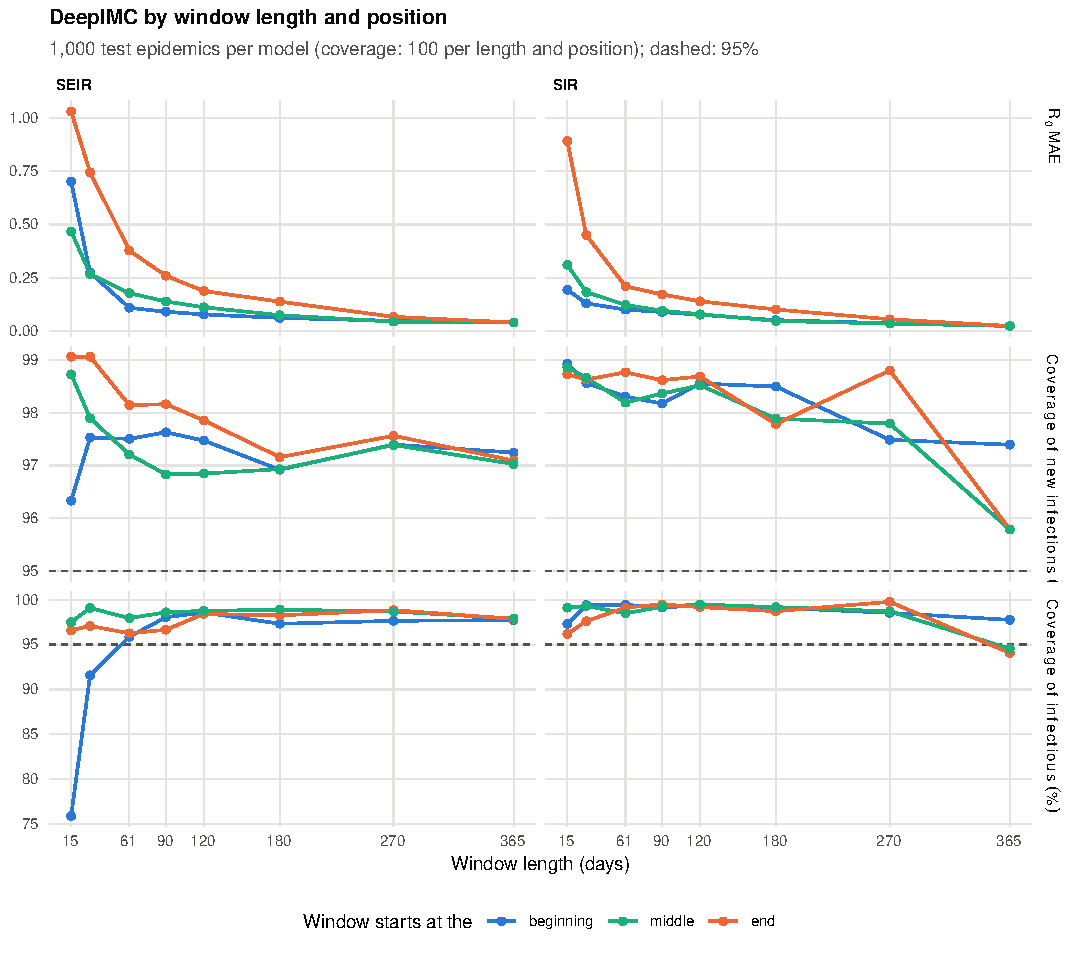
\includegraphics[width=\textwidth]{figures/deepimc_by_window.pdf}
\caption{DeepIMC by window length and position: $R_0$ mean absolute error, and coverage of the true daily
new infections and of the true number currently infectious by the 95\% band, for windows that start at the
beginning, the middle and the end of the test epidemics.}
\label{fig:deepimc-by-window}
\end{figure}

\paragraph{The epidemic behind the window.} When the model is run forward from DeepIMC's estimates, the
true daily new infections fall inside the 95\% band on 96--99\% of the days at every window length, and the
true number of infectious people---which the network never sees---on 90--99\% of the days. DeepIMC
therefore recovers not only $R_0$ but also the hidden state of the epidemic. Its estimates of the transmission
probability and the contact rate are discussed with the comparison methods below.

\subsection{Parameter recovery compared with standard methods}\label{sec:res-sim-params}

We now turn to the comparison with the four standard methods on the 10,000 simulated test windows. The
first question is how accurately each method recovers the parameters and the starting state.

\paragraph{$R_0$.} DeepIMC estimated $R_0$ with a mean absolute error of 0.19 in both the SEIR and the SIR
windows (Table~\ref{tab:sim-parameters}). The best comparison method was ABC-SMC for SEIR (0.61) and
differential evolution for SIR (0.49), so DeepIMC's error was about three times smaller for SEIR and 2.6 times
smaller for SIR. ABC-MCMC (0.88 and 0.84) and Nelder--Mead (0.93 and 0.92) were the least accurate. On the same
windows, every comparison method had a larger error than DeepIMC, for every position of the window, and none of
the 95\% bootstrap intervals of the paired differences lies below zero (Table~\ref{tab:sim-paired}). DeepIMC
was more accurate than ABC-SMC on 83\% (SEIR) and 80\% (SIR) of the windows, and more accurate than
differential evolution on 76\% and 74\%.

\paragraph{The position and the length of the window.} Where the window comes from matters a great deal for the
comparison methods. On early windows, which contain the growth of the epidemic, differential evolution came
closest to DeepIMC (0.27 against 0.14 for SEIR, 0.23 against 0.12 for SIR). On middle and late windows, where a
method must also work out how many people were already infected or immune, the errors of the comparison methods
were two to four times larger than on early windows, while DeepIMC's errors grew much less (to 0.17 and 0.27 for
SEIR, 0.17 and 0.28 for SIR). Figure~\ref{fig:methods-by-window} breaks these results down by window length as
well: DeepIMC had the lowest $R_0$ error in all 30 groups of length and position. Windows of 15 to 29 days were
hard for every method, but least for DeepIMC (0.46 for SEIR and 0.28 for SIR, against 0.71 to 1.46 for the
others). The longest windows, of 180 to 365 days, contain most of the epidemic, and there differential evolution
and Nelder--Mead became much more accurate (0.12 to 0.21), though still less than DeepIMC (0.07 and 0.04). Longer
windows helped every method except ABC-MCMC, whose error grew with the length of SIR windows (from 0.70 to 1.69).
Figure~\ref{fig:parameter-recovery} shows how the comparison methods fail: ABC-MCMC's estimates are pulled
towards the middle of the range, ABC-SMC underestimates many large values of $R_0$, and differential evolution
and Nelder--Mead return many estimates at the lower limit of 0.8 whatever the true value.

\paragraph{The range of $R_0$.} DeepIMC's 95\% range contained the true $R_0$ in 96\% (SEIR) and 97\% (SIR) of
the windows, close to the nominal 95\%, with an average width of 0.98 and 0.93. The ranges of ABC-MCMC and
ABC-SMC contained it about as often (95--97\%), but they were three to four times wider (2.8 to 3.6, for a prior
range of width 4.2): they were rarely wrong because they said little.

\paragraph{The transmission probability and the contact rate.} As expected from Section~\ref{sec:models}, no
method recovered $p_{tran}$ and $c_{rate}$ separately (Figure~\ref{fig:parameter-recovery}, rows $p_{tran}$ and
$c_{rate}$). DeepIMC's errors were close to those of the guess that knows $R_0$ exactly and takes the middle of
the range of the contact rate: 0.0148 against 0.0140 for $p_{tran}$ in SEIR windows (0.0709 against 0.0734 in
SIR windows), and 2.58 against 2.51 for $c_{rate}$ (1.05 against 1.01). The comparison methods fix $c_{rate}$ at
the middle of its range, so their $c_{rate}$ error is that of the guess by construction; their $p_{tran}$ errors
are larger than DeepIMC's because their $R_0$ is less accurate. The curve contains information about $R_0$, the
product of the two, but none about how it splits.

\paragraph{The starting state.} The error of the estimated shares exposed, infectious and recovered at the start
of the window was 1.5 (SEIR) and 2.7 (SIR) percentage points for DeepIMC, against 4.3 to 9.7 and 5.4 to 14.1 for
the comparison methods. ABC-SMC failed on 18 SEIR and 2 SIR windows even with its raised limits; they are left
out of its averages.

\begin{table}[htbp]
\centering
\caption{Parameter recovery on the 10,000 simulated test windows (5,000 per model). MAE of $R_0$ for all
windows and for early, middle and late windows; for the methods that give a 95\% range of $R_0$, the
percentage of windows whose range contains the true value and the average width of the range; MAE of
$p_{tran}$ and $c_{rate}$, with the error of a guess that knows $R_0$ exactly and takes the middle of the
range of $c_{rate}$; starting-state error (percentage points). Bold: lowest error. The comparison methods
fix $c_{rate}$ at the middle of its range, so their $c_{rate}$ error is that of the guess. Weighted DeepIMC keeps
DeepIMC's $R_0$ and range; only its starting state differs.}
\label{tab:sim-parameters}
\small
\resizebox{\textwidth}{!}{\begin{tabular}{llrrrrrrrrr}
\toprule
 &  & \multicolumn{4}{c}{$R_0$ MAE} & \multicolumn{2}{c}{95\% range of $R_0$} & $p_{tran}$ & $c_{rate}$ & State \\
\cmidrule(lr){3-6}\cmidrule(lr){7-8}
Model & Method & all & early & middle & late & has true (\%) & width & MAE & MAE & error \\
\midrule
SEIR & DeepIMC & \textbf{0.19} & \textbf{0.14} & \textbf{0.17} & \textbf{0.27} & 96.2 & 0.98 & 0.0148 & 2.58 & 1.5 \\
 & DeepIMC, weighted & 0.19 & 0.14 & 0.17 & 0.27 & 96.2 & 0.98 & 0.0148 & 2.58 & \textbf{1.2} \\
 & ABC-MCMC & 0.88 & 0.75 & 0.88 & 1.00 & 94.8 & 3.56 & 0.0202 & 2.51 & 9.0 \\
 & ABC-SMC & 0.61 & 0.37 & 0.61 & 0.85 & 97.1 & 2.98 & 0.0178 & 2.51 & 5.0 \\
 & DE & 0.63 & 0.27 & 0.67 & 0.96 & -- & -- & 0.0190 & 2.51 & 4.3 \\
 & Nelder--Mead & 0.93 & 0.52 & 0.99 & 1.28 & -- & -- & 0.0222 & 2.51 & 9.7 \\
 & \textit{guess knowing $R_0$} &  &  &  &  &  &  & 0.0140 & 2.51 &  \\
\midrule
SIR & DeepIMC & \textbf{0.19} & \textbf{0.12} & \textbf{0.17} & \textbf{0.28} & 96.6 & 0.93 & 0.0709 & 1.05 & 2.7 \\
 & DeepIMC, weighted & 0.19 & 0.12 & 0.17 & 0.28 & 96.6 & 0.93 & 0.0709 & 1.05 & \textbf{2.2} \\
 & ABC-MCMC & 0.84 & 0.72 & 0.86 & 0.95 & 96.0 & 3.45 & 0.0842 & 1.01 & 14.1 \\
 & ABC-SMC & 0.54 & 0.27 & 0.49 & 0.85 & 97.3 & 2.78 & 0.0778 & 1.01 & 7.3 \\
 & DE & 0.49 & 0.23 & 0.49 & 0.76 & -- & -- & 0.0772 & 1.01 & 5.4 \\
 & Nelder--Mead & 0.92 & 0.36 & 1.05 & 1.36 & -- & -- & 0.0950 & 1.01 & 11.9 \\
 & \textit{guess knowing $R_0$} &  &  &  &  &  &  & 0.0734 & 1.01 &  \\
\bottomrule
\end{tabular}
}
\end{table}

\begin{table}[htbp]
\centering
\caption{Paired difference in the $R_0$ absolute error, comparison method minus DeepIMC, on the same
windows (positive: DeepIMC is more accurate), with 95\% bootstrap intervals.}
\label{tab:sim-paired}
\small
\resizebox{\textwidth}{!}{\begin{tabular}{llllll}
\toprule
Model & Method & All windows & Early & Middle & Late \\
\midrule
SEIR & ABC-MCMC & 0.68 (0.67, 0.70) & 0.61 (0.58, 0.64) & 0.71 (0.68, 0.75) & 0.73 (0.69, 0.76) \\
 & ABC-SMC & 0.41 (0.40, 0.43) & 0.23 (0.21, 0.25) & 0.44 (0.41, 0.47) & 0.58 (0.54, 0.61) \\
 & DE & 0.44 (0.42, 0.46) & 0.13 (0.11, 0.15) & 0.51 (0.47, 0.54) & 0.69 (0.64, 0.73) \\
 & Nelder--Mead & 0.73 (0.70, 0.76) & 0.37 (0.35, 0.40) & 0.83 (0.78, 0.88) & 1.00 (0.95, 1.06) \\
\midrule
SIR & ABC-MCMC & 0.65 (0.63, 0.67) & 0.60 (0.57, 0.62) & 0.70 (0.66, 0.73) & 0.66 (0.63, 0.70) \\
 & ABC-SMC & 0.35 (0.33, 0.36) & 0.15 (0.14, 0.16) & 0.32 (0.30, 0.35) & 0.57 (0.53, 0.60) \\
 & DE & 0.30 (0.28, 0.32) & 0.11 (0.10, 0.13) & 0.32 (0.29, 0.35) & 0.47 (0.44, 0.51) \\
 & Nelder--Mead & 0.73 (0.70, 0.75) & 0.24 (0.22, 0.27) & 0.88 (0.82, 0.94) & 1.08 (1.02, 1.13) \\
\bottomrule
\end{tabular}
}
\end{table}

\begin{figure}[htbp]
\centering
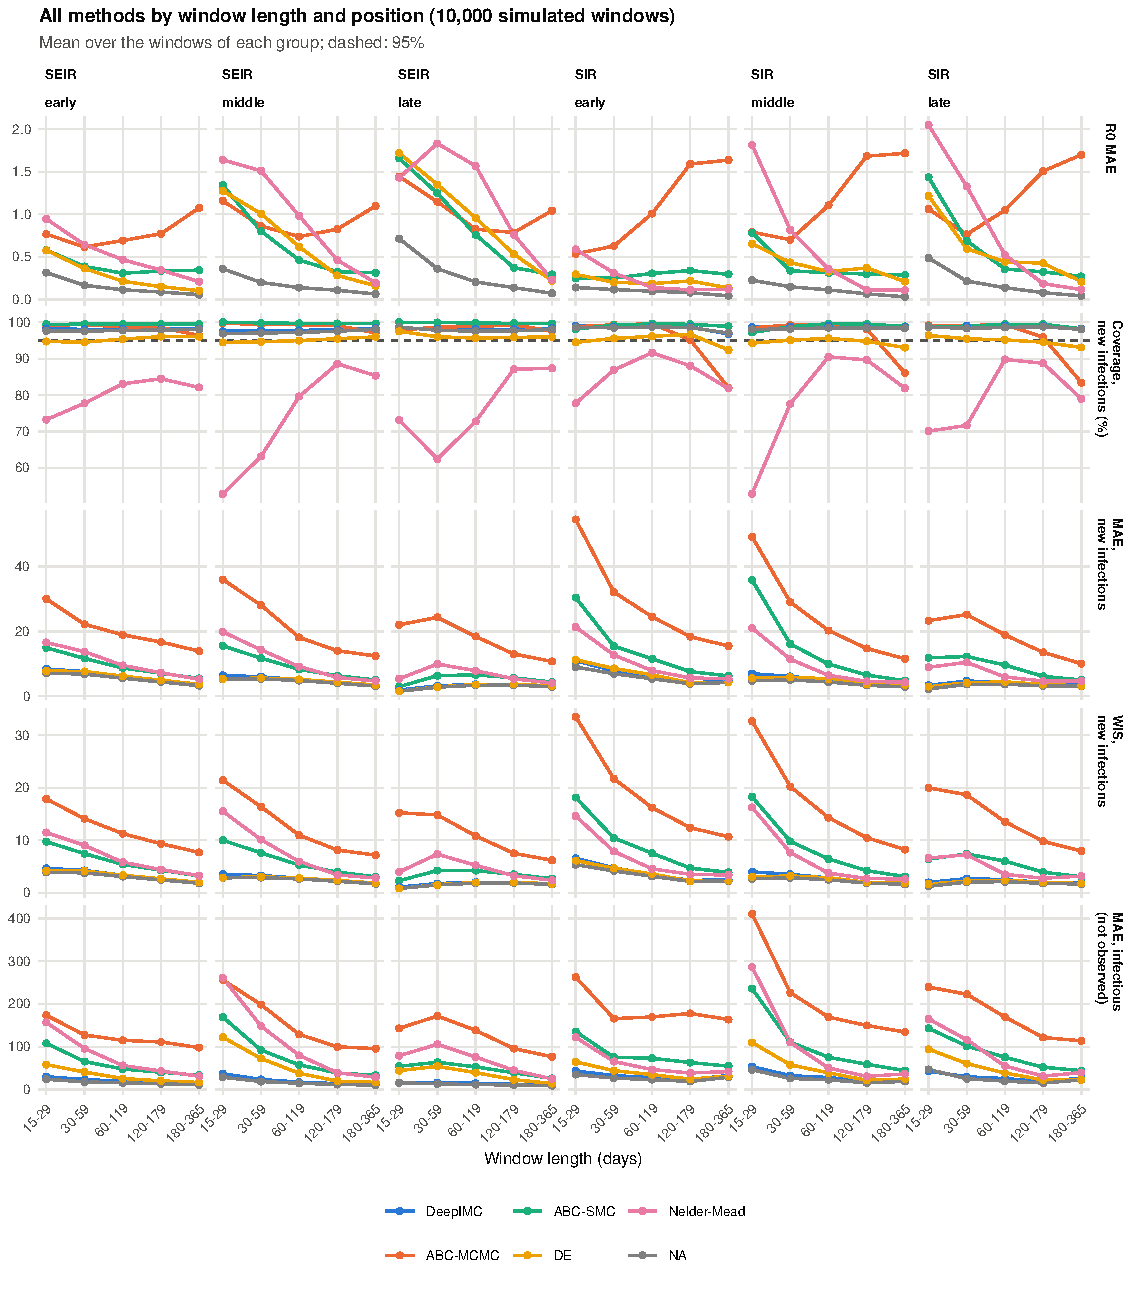
\includegraphics[width=\textwidth]{figures/methods_by_window_simulated.pdf}
\caption{All methods on the 10,000 simulated test windows, by window length and position
(early, middle, late): $R_0$ mean absolute error; coverage of the true daily new infections in the window by
the 95\% band; MAE and WIS of the regenerated daily new infections in the window; and MAE of the regenerated
number currently infectious (not observed by any method). Dashed line: 95\%.}
\label{fig:methods-by-window}
\end{figure}

\begin{figure}[htbp]
\centering
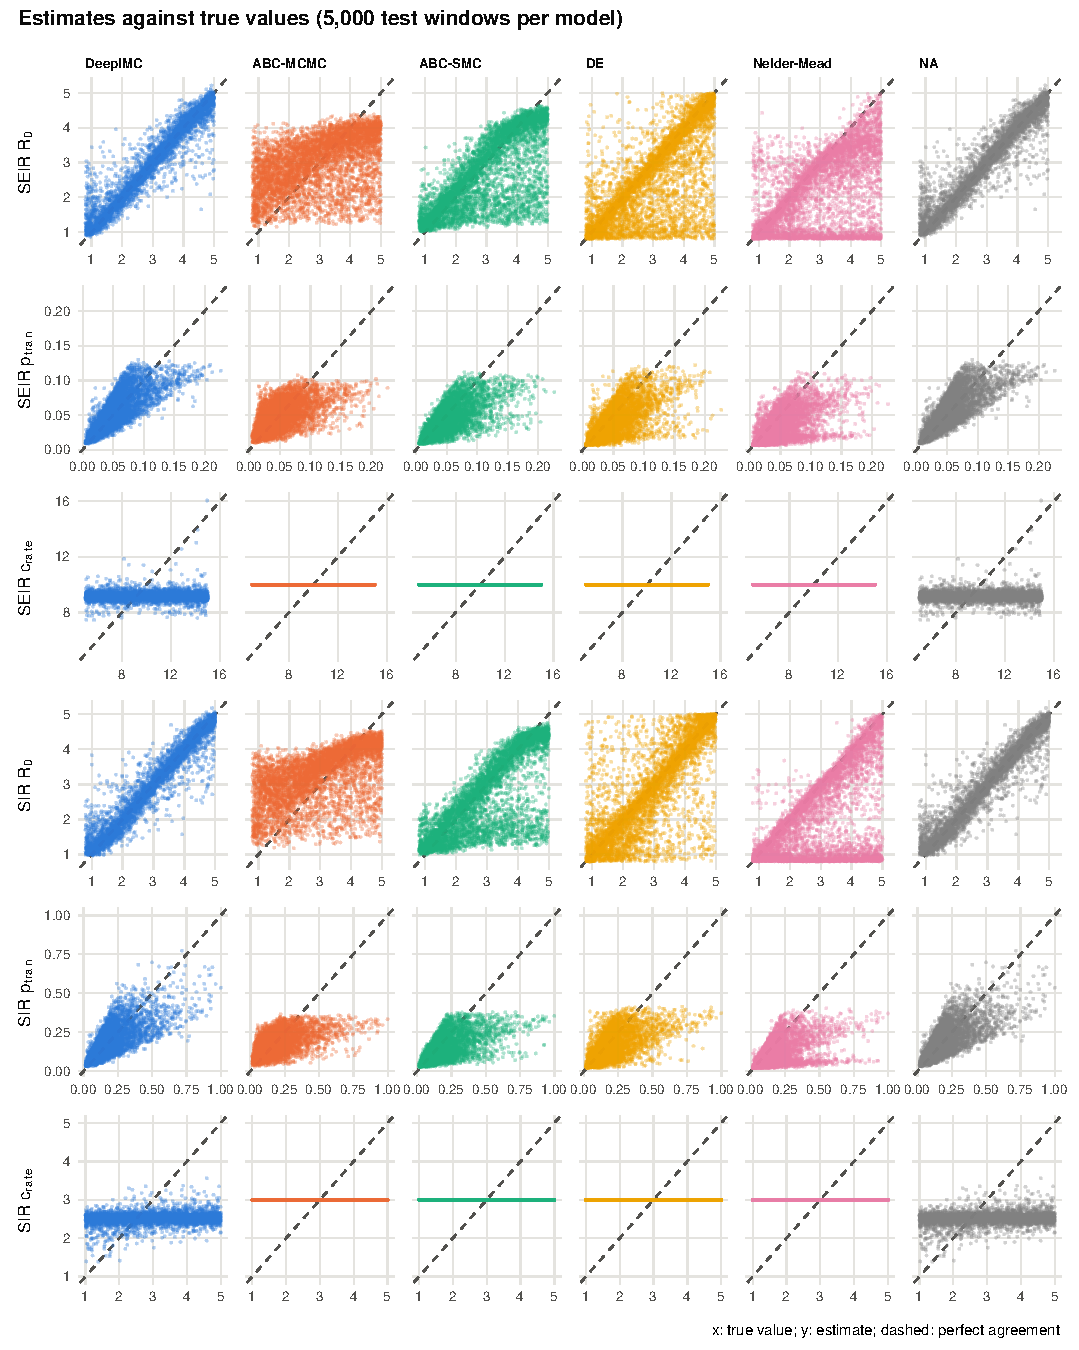
\includegraphics[width=\textwidth]{figures/parameter_recovery.pdf}
\caption{Estimated against true values of $R_0$, $p_{tran}$ and $c_{rate}$ for every simulated test
window and method; the dashed line is perfect agreement. DeepIMC's flat cloud for $c_{rate}$ shows that the
curve does not reveal it; the comparison methods fix it at the middle of its range.}
\label{fig:parameter-recovery}
\end{figure}

\subsection{Recovery of the epidemic curves}\label{sec:res-sim-curves}

The second question is whether each method's estimates reproduce the epidemic itself.

For each window, we ran the agent-based model 500 times from each method's estimates and compared the
regenerated curves with the true curves of the test epidemic (Table~\ref{tab:sim-curves},
Figures~\ref{fig:heatmap-sim}--\ref{fig:ridgelines}).

\paragraph{New infections in the window.} All methods except Nelder--Mead reproduced the curve they had seen.
The MAE of the regenerated median curve was 4.8 daily new infections for both DeepIMC and differential
evolution in the SEIR windows (6.2 and 6.1 in the SIR windows), against 8.1 to 19.8 for the ABC methods (17.2
to 31.3) and 9.3 for Nelder--Mead (12.2); the WIS, which also rewards honest bands, gave the same ranking (2.6
for both DeepIMC and differential evolution in SEIR windows, 3.6 and 3.3 in SIR windows). Differential
evolution, which fits each window directly, came as close to the data as DeepIMC, and slightly closer in middle
and late windows. DeepIMC's bands covered 98--99\% of the days, those of differential evolution 95\%, those of
the ABC methods 99--100\% and those of Nelder--Mead 77--78\%.

\paragraph{The number currently infectious.} This curve, which no method observes, depends on the estimated
starting state as well as on $R_0$, and it is where the methods differed most. DeepIMC's bands covered the true
number of infectious people on 98--99\% of the days, and its median curve was off by 18 people on average in the
SEIR windows and 35 in the SIR windows---about half the error of the best comparison method, differential
evolution (39 and 61); by the WIS, DeepIMC's error was a third (SEIR) and 43\% (SIR) of that method's.
Differential evolution and Nelder--Mead, which return a single estimate, covered the true number on only 73--78\%
and 53--58\% of the days, and below 80\% in 37--43\% of the windows for differential evolution and 60--72\% for
Nelder--Mead, against 2\% for DeepIMC (Figure~\ref{fig:ridgelines}). The ABC methods covered it on 99--100\% of
the days, with errors three to seven times larger than DeepIMC's.

\paragraph{The next 14 days.} Two weeks beyond the window, the curves regenerated from DeepIMC were the closest
to the truth (MAE 1.8 new infections per day for SEIR and 1.0 for SIR, WIS 1.0 and 0.6), followed by
differential evolution (2.0 and 1.2) and ABC-SMC (2.5 and 1.3); all methods except Nelder--Mead covered
96--100\% of the days. Many test windows end when the epidemic is already declining, so the counts over these
days are small. Figure~\ref{fig:curve-recovery} shows three typical SEIR windows and the distribution of the
errors over all windows.

\paragraph{Weighted DeepIMC.} Keeping the 10\% of DeepIMC's draws closest to each window
(Section~\ref{sec:weighting}) improved the curves in 95\% of the simulated windows (Table~\ref{tab:sim-curves}). The
new infections in the window were then reproduced more closely than by differential evolution (MAE 4.4 against
4.8 for SEIR, 5.1 against 6.1 for SIR; WIS 2.4 against 2.6 and 2.9 against 3.3), the starting state was more
accurate (an error of 1.2 and 2.2 percentage points instead of 1.5 and 2.7), and the number currently infectious
was closer to the truth (WIS 8.8 and 18.2 instead of 10.7 and 20.7), with a coverage of 96--98\%. The cumulative
error fell to 1.9\% (SEIR) and 2.3\% (SIR) of the final count, the lowest of all methods. In only one of the
10,000 simulated windows did no draw reproduce the window within twice the Poisson noise.

\begin{table}[htbp]
\centering
\caption{Recovery of the epidemic curves on the 10,000 simulated test windows: coverage (\%), MAE and WIS
of the true daily new infections in the window, of the true number currently infectious in the window
(not observed by any method), and of the daily new infections in the 14 days after the window, from 500
model runs per window and method.}
\label{tab:sim-curves}
\small
\resizebox{\textwidth}{!}{\begin{tabular}{llrrrrrrrrr}
\toprule
 &  & \multicolumn{3}{c}{New infections, window} & \multicolumn{3}{c}{Infectious, window} & \multicolumn{3}{c}{New infections, next 14 days} \\
\cmidrule(lr){3-5}\cmidrule(lr){6-8}\cmidrule(lr){9-11}
Model & Method & Cov. (\%) & MAE & WIS & Cov. (\%) & MAE & WIS & Cov. (\%) & MAE & WIS \\
\midrule
SEIR & DeepIMC & 98.1 & 4.8 & 2.6 & 98.4 & 17.9 & 10.7 & 98.8 & 1.8 & 1.0 \\
 & DeepIMC, weighted & 97.6 & \textbf{4.4} & \textbf{2.4} & \textbf{97.9} & \textbf{14.7} & \textbf{8.7} & 98.4 & \textbf{1.7} & \textbf{0.9} \\
 & ABC-MCMC & 98.7 & 19.8 & 11.8 & 98.7 & 134.1 & 79.4 & 98.6 & 6.2 & 3.7 \\
 & ABC-SMC & 99.7 & 8.1 & 5.1 & 99.7 & 59.1 & 37.6 & 99.5 & 2.5 & 1.5 \\
 & DE & \textbf{95.5} & 4.8 & 2.6 & 78.2 & 39.0 & 30.6 & \textbf{96.6} & 2.0 & 1.1 \\
 & Nelder--Mead & 76.9 & 9.3 & 6.2 & 52.9 & 81.7 & 70.4 & 79.4 & 5.8 & 4.1 \\
\midrule
SIR & DeepIMC & 98.8 & 6.2 & 3.6 & 98.7 & 35.1 & 20.7 & 99.1 & 1.0 & 0.6 \\
 & DeepIMC, weighted & 98.4 & \textbf{5.1} & \textbf{2.9} & \textbf{95.6} & \textbf{30.2} & \textbf{18.2} & 98.8 & \textbf{0.9} & \textbf{0.5} \\
 & ABC-MCMC & 98.8 & 31.3 & 21.6 & 98.7 & 227.6 & 139.1 & 99.0 & 2.7 & 2.3 \\
 & ABC-SMC & 98.8 & 17.2 & 10.2 & 99.0 & 114.3 & 66.5 & 99.5 & 1.3 & 0.8 \\
 & DE & \textbf{95.3} & 6.1 & 3.3 & 73.1 & 61.1 & 48.0 & \textbf{97.4} & 1.2 & 0.7 \\
 & Nelder--Mead & 77.5 & 12.2 & 8.3 & 57.9 & 115.8 & 99.9 & 88.6 & 3.1 & 1.9 \\
\bottomrule
\end{tabular}
}
\end{table}

\begin{figure}[htbp]
\centering
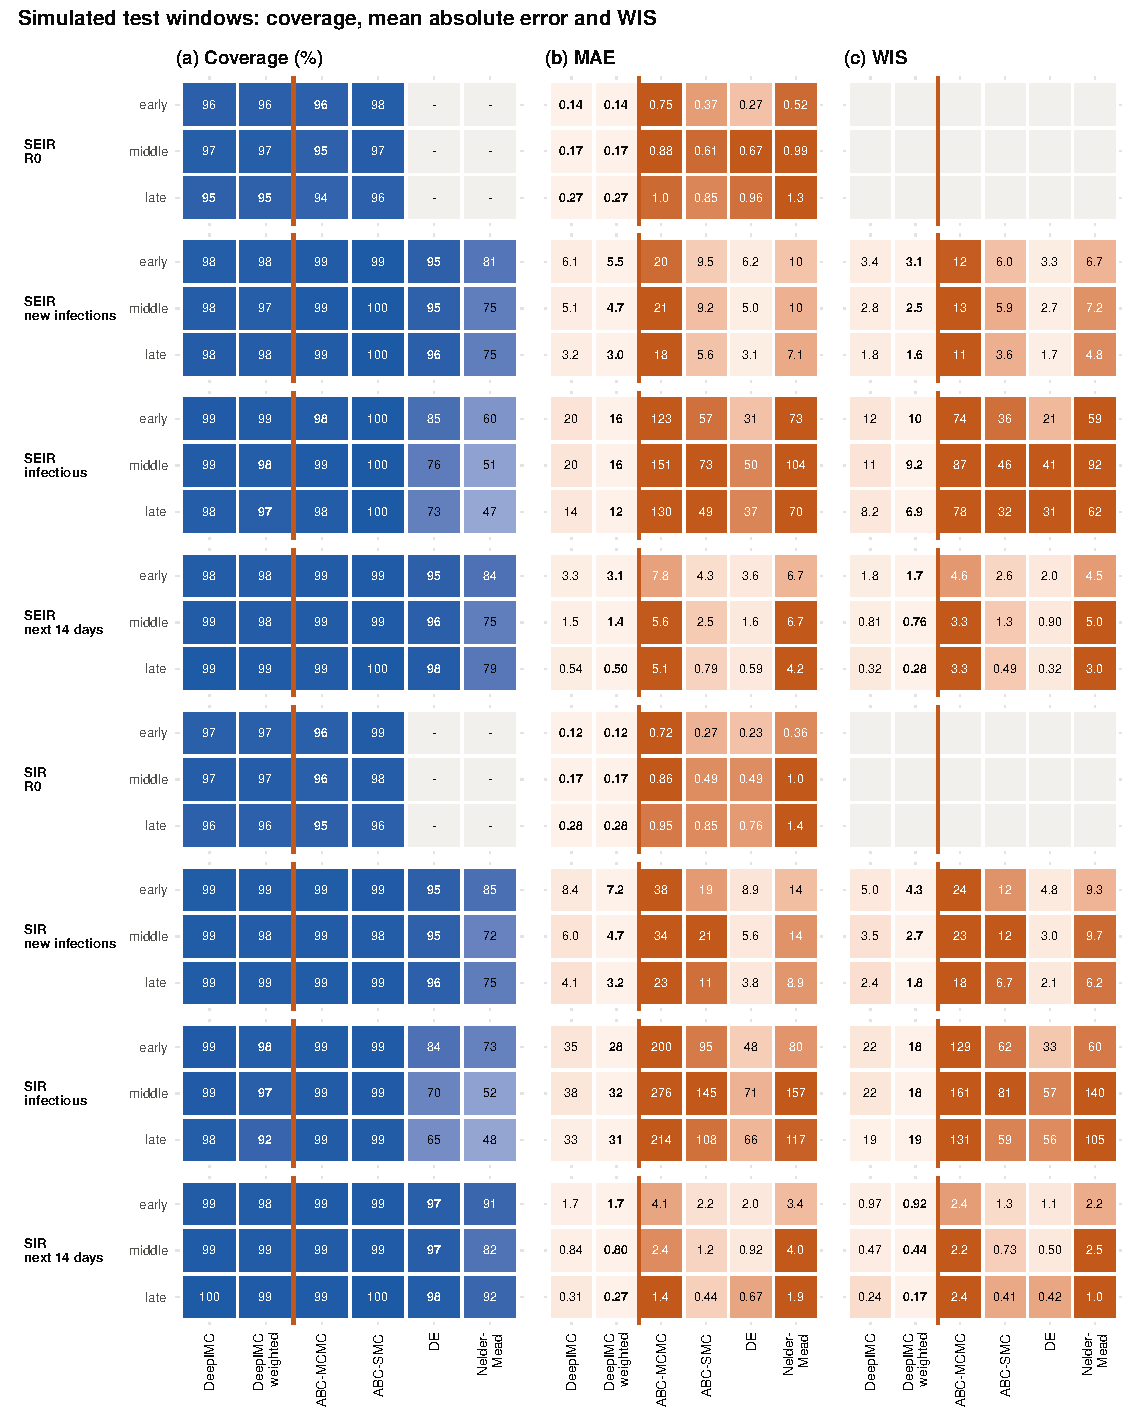
\includegraphics[width=\textwidth]{figures/coverage_mae_simulated.pdf}
\caption{Simulated test windows. (a) Mean coverage by method, for early, middle and late windows: of
the true $R_0$ by the 95\% range, and of the true curves by the 95\% band (bold: closest to 95\%;
``-'': the method gives no range). (b) Mean absolute error of $R_0$ and of the regenerated curves and (c) mean
weighted interval score of the curves (bold: lowest).}
\label{fig:heatmap-sim}
\end{figure}

\begin{figure}[htbp]
\centering
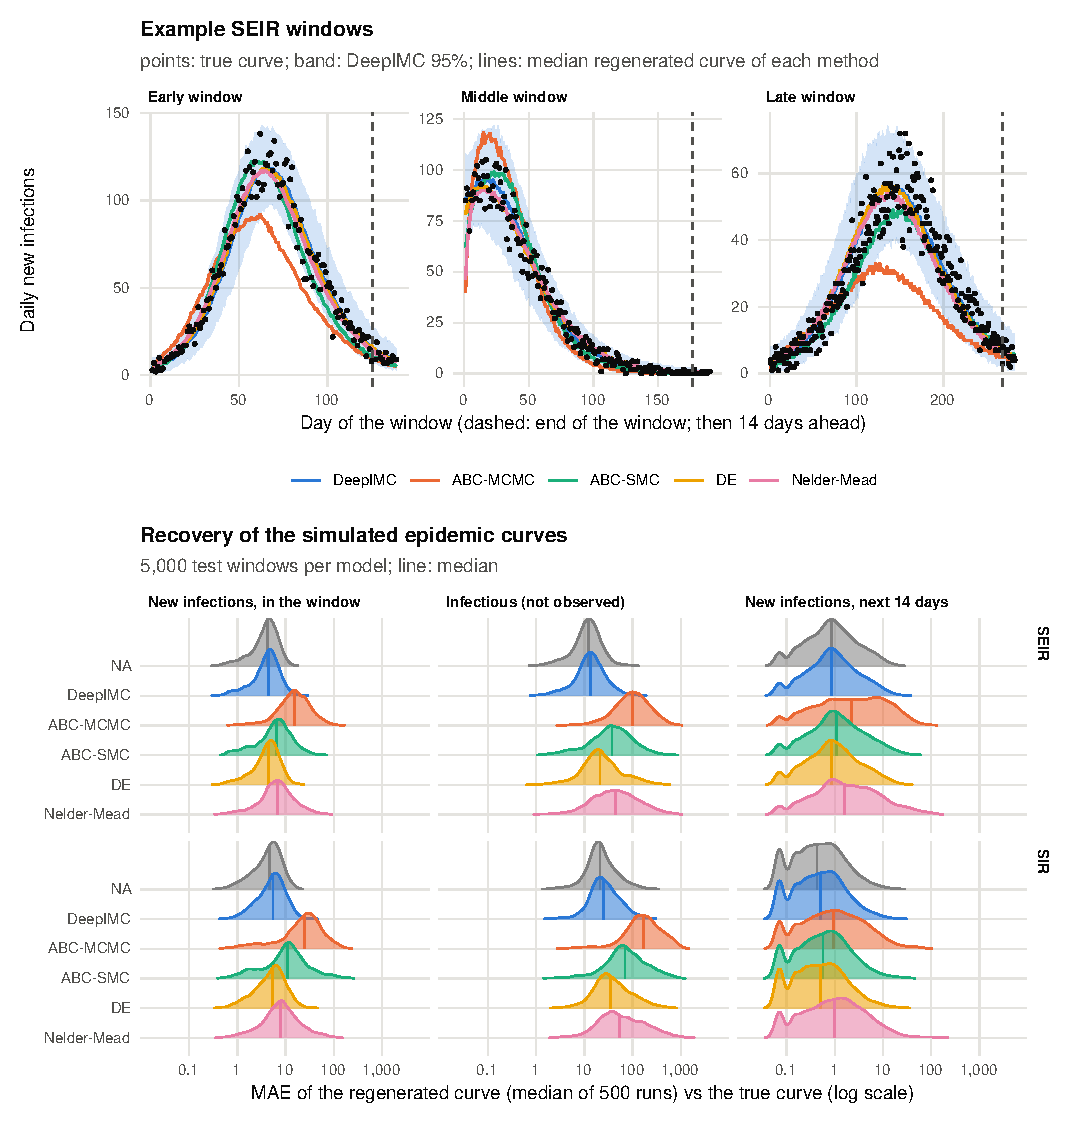
\includegraphics[width=\textwidth]{figures/curve_recovery.pdf}
\caption{Recovery of the simulated epidemic curves. Top: three SEIR test windows (early, middle and late)
with the true curve (points), DeepIMC's 95\% band and every method's median regenerated curve; the dashed
line marks the end of the window. Bottom: distribution over all test windows of the MAE of the median
regenerated curve (log scale; vertical line: median).}
\label{fig:curve-recovery}
\end{figure}

\begin{figure}[htbp]
\centering
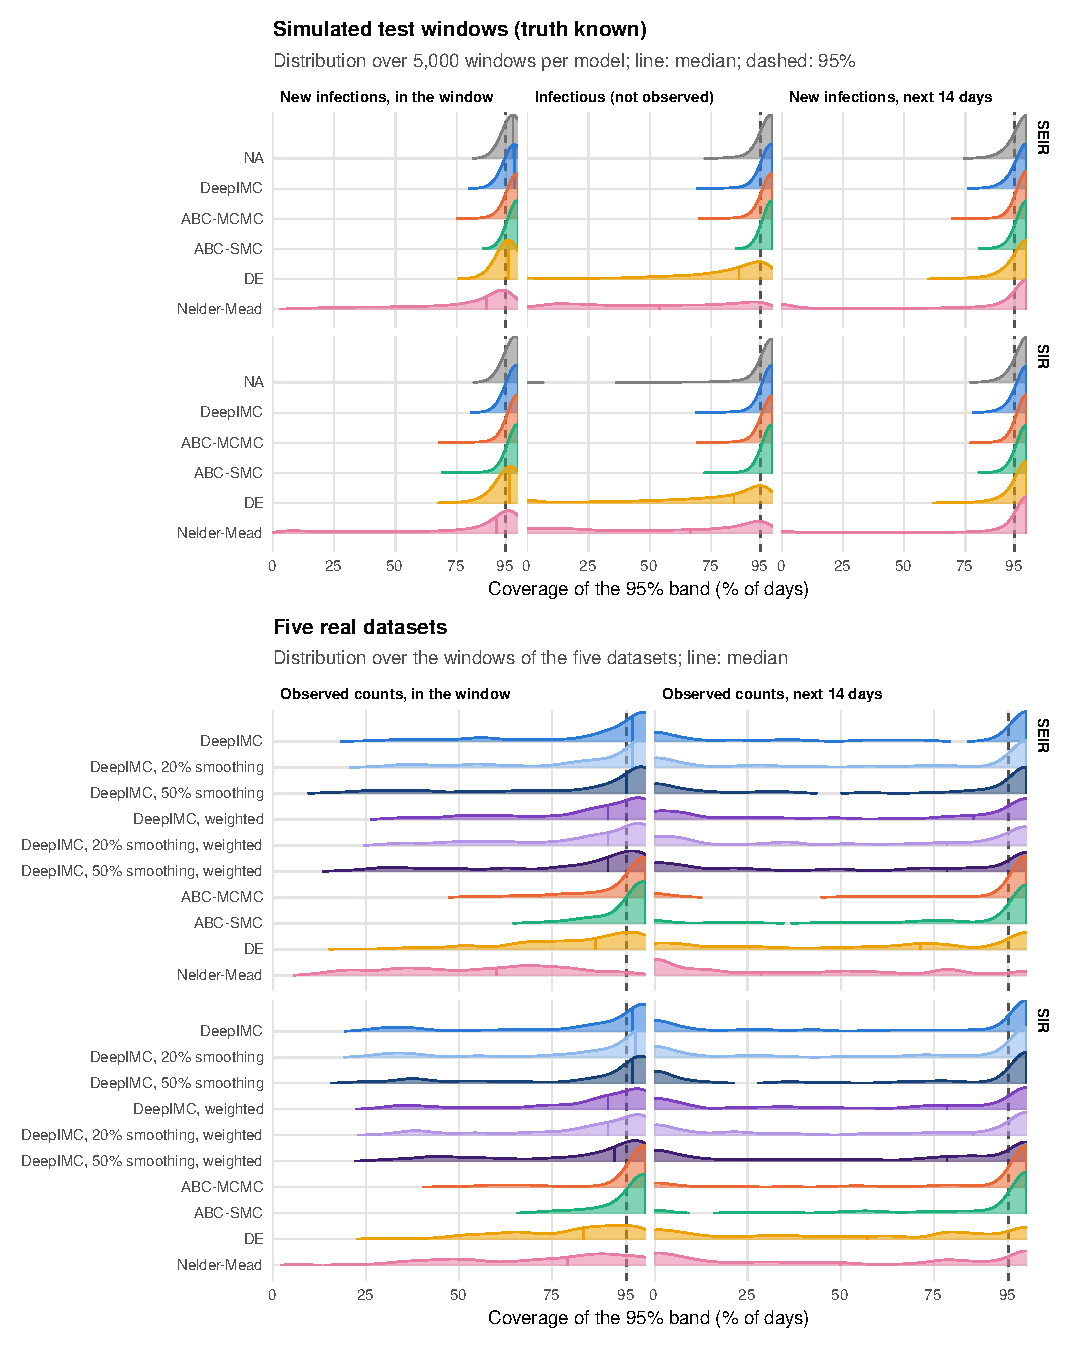
\includegraphics[width=\textwidth]{figures/coverage_ridgelines.pdf}
\caption{Distribution of the coverage of the 95\% band over the windows, by method: simulated test
windows (top) and the five real datasets (bottom). Vertical line in each ridge: median; dashed: 95\%.}
\label{fig:ridgelines}
\end{figure}

\paragraph{DeepIMC against each method.} Figure~\ref{fig:ratios-sim} compares DeepIMC with each method in turn,
on the same windows. DeepIMC's MAE and WIS were lower than those of every comparison method, in every position
and for every curve, with one exception: the new infections in the window, which differential evolution fits
directly, where the two methods were equal within about 10\% (ratios of 0.95 to 1.1). For the number currently
infectious, DeepIMC's WIS was 26--66\% of that of differential evolution. Its coverage was about the same as that
of the ABC methods, which reach it with much wider bands, and 1.2 to 1.5 times that of differential evolution for
the number currently infectious (up to twice that of Nelder--Mead).

\begin{figure}[htbp]
\centering
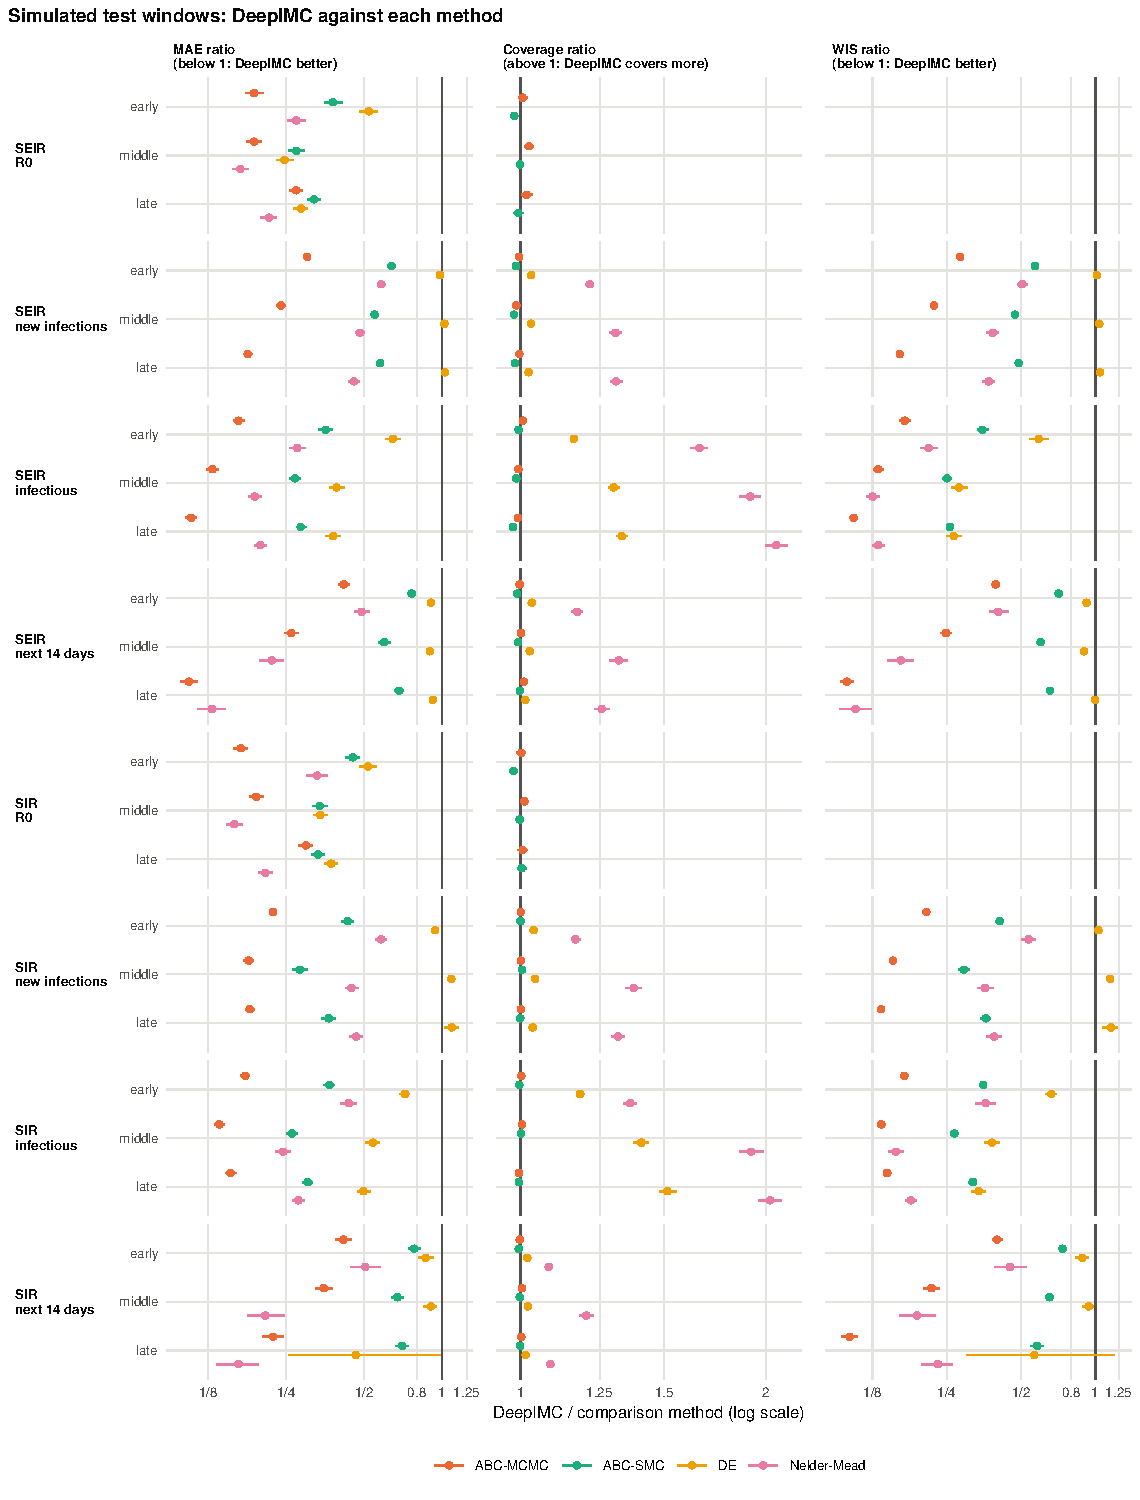
\includegraphics[width=\textwidth]{figures/ratios_simulated.pdf}
\caption{Simulated test windows: DeepIMC's mean MAE, mean coverage and mean WIS divided by those of each
comparison method on the same windows, for early, middle and late windows, with 95\% bootstrap intervals over
the windows (log scale). MAE and WIS ratios below 1 and coverage ratios above 1 favour DeepIMC; the coverage of
$R_0$ is that of the 95\% range, given only by DeepIMC and the ABC methods.}
\label{fig:ratios-sim}
\end{figure}

\paragraph{Cumulative incidence.} Adding up the daily new infections tells the same story
(Table~\ref{tab:sim-cumulative}). The cumulative curves regenerated from DeepIMC and from differential evolution
were the closest to the truth (an error of 3.5\% and 3.2\% of the final count in SEIR windows, 8.9\% and 5.4\% in
SIR windows), against 10.8--90\% for the ABC methods; but DeepIMC's band contained the true cumulative count on
98--99\% of the days, and that of differential evolution on only 61--83\%. Over the next 14 days DeepIMC's
cumulative error was 6.2\% (SEIR) and 13.0\% (SIR), against 5.2\% and 27.9\% for differential evolution.

\begin{table}[htbp]
\centering
\caption{Simulated test windows: the cumulative new infections since the first day of the window (an
evaluation only; every method is fitted to the daily counts). Coverage of the true cumulative curve by the
95\% band, its MAE as a percentage of the true final count, and its WIS; in the window and over the next 14
days.}
\label{tab:sim-cumulative}
\small
\resizebox{\textwidth}{!}{\begin{tabular}{llrrrrrr}
\toprule
 &  & \multicolumn{3}{c}{Window} & \multicolumn{3}{c}{Next 14 days} \\
\cmidrule(lr){3-5}\cmidrule(lr){6-8}
Model & Method & Cov. (\%) & Rel.\ MAE (\%) & WIS & Cov. (\%) & Rel.\ MAE (\%) & WIS \\
\midrule
SEIR & DeepIMC & \textbf{98.9} & 3.5 & 36.8 & \textbf{97.7} & 6.2 & 46.8 \\
 & DeepIMC, weighted & 99.4 & \textbf{1.9} & \textbf{23.7} & 98.6 & \textbf{2.9} & \textbf{27.6} \\
 & ABC-MCMC & 99.3 & 90.4 & 390.8 & 98.1 & 174.7 & 550.2 \\
 & ABC-SMC & 99.8 & 10.8 & 150.2 & 99.3 & 18.4 & 201.7 \\
 & DE & 77.9 & 3.2 & 35.4 & 61.3 & 5.2 & 49.5 \\
 & Nelder--Mead & 38.6 & 14.3 & 168.8 & 34.5 & 31.2 & 231.3 \\
\midrule
SIR & DeepIMC & \textbf{99.1} & 8.9 & 48.0 & \textbf{98.4} & 13.0 & 55.7 \\
 & DeepIMC, weighted & 99.6 & \textbf{2.3} & \textbf{23.4} & 98.8 & \textbf{3.2} & \textbf{24.8} \\
 & ABC-MCMC & 99.3 & 71.1 & 451.1 & 99.5 & 131.4 & 604.4 \\
 & ABC-SMC & 99.6 & 20.4 & 190.6 & 99.6 & 26.7 & 230.6 \\
 & DE & 82.9 & 5.4 & 28.5 & 68.3 & 27.9 & 38.3 \\
 & Nelder--Mead & 56.6 & 10.3 & 101.9 & 48.7 & 18.4 & 129.4 \\
\bottomrule
\end{tabular}
}
\end{table}

\subsection{The starting state}\label{sec:res-start}

The window rarely starts at the beginning of an epidemic, so the starting state matters for every prediction.
Two questions follow: does estimating the starting state help, and is DeepIMC's estimate better than one fitted
to the window by the renewal equation?

\paragraph{Estimating the state or assuming it.} We regenerated every window twice from the same estimates of
$R_0$: once from DeepIMC's estimated state, and once from the state a user without such an estimate would assume,
treating the window as the start of the epidemic (nobody recovered, and the infected and exposed counts equal to
the first day's count). The naive start was far worse (Table~\ref{tab:state-ablation}). On the simulated
windows, its band covered the first week of the window on 14\% (SEIR) and 28\% (SIR) of the days and the whole
window on 33\% and 46\%, against 98--99\% from DeepIMC's state, with MAEs ten times larger. On the real windows
the same pattern held: from DeepIMC's state the band covered 92\% of the first week and 85--86\% of the window,
from the naive state 40--41\% and 55--61\%, with three times the error in the first week. Over the 14 days after
a real window, however, the two starts gave similar results (coverage 68--69\% from DeepIMC's state and 75--78\%
from the naive one, with similar MAEs): beyond the window, the changes of a real epidemic matter more than the
state it started from.

\begin{table}[htbp]
\centering
\caption{The same DeepIMC estimates of $R_0$ started from DeepIMC's estimated state or from a naive state (the
window is treated as the start of the epidemic: nobody has recovered, and the infected and exposed counts equal
the first day's count): coverage (\%) and MAE of the daily counts in the first 7 days of the window, in the whole
window and in the next 14 days. Simulated: 1,000 test windows (500 per model); real: the windows of the five
datasets.}
\label{tab:state-ablation}
\small
\resizebox{\textwidth}{!}{\begin{tabular}{lllrrrrrr}
\toprule
 &  &  & \multicolumn{2}{c}{First 7 days} & \multicolumn{2}{c}{Whole window} & \multicolumn{2}{c}{Next 14 days} \\
\cmidrule(lr){4-5}\cmidrule(lr){6-7}\cmidrule(lr){8-9}
Data & Model & Starting state & Cov. (\%) & MAE & Cov. (\%) & MAE & Cov. (\%) & MAE \\
\midrule
Simulated & SEIR & DeepIMC & 98.0 & 5.3 & 98.0 & 4.7 & 99.1 & 1.8 \\
 &  & naive & 14.1 & 44.5 & 33.3 & 43.9 & 54.1 & 31.0 \\
\cmidrule(lr){2-9}
 & SIR & DeepIMC & 99.2 & 11.4 & 98.8 & 6.2 & 98.9 & 1.0 \\
 &  & naive & 27.5 & 106.8 & 46.4 & 89.1 & 75.7 & 23.1 \\
\midrule
Real & SEIR & DeepIMC & 92.1 & 6.0 & 86.4 & 13.6 & 69.0 & 22.2 \\
 &  & naive & 41.0 & 21.1 & 54.5 & 24.2 & 75.4 & 24.8 \\
\cmidrule(lr){2-9}
 & SIR & DeepIMC & 91.6 & 7.0 & 84.7 & 13.1 & 67.8 & 19.7 \\
 &  & naive & 39.6 & 21.9 & 61.3 & 20.7 & 77.5 & 19.9 \\
\bottomrule
\end{tabular}
}
\end{table}

\paragraph{DeepIMC's state or the renewal equation's.} The renewal equation can also supply the starting
state, by fitting it to the window given DeepIMC's $R_0$ (Table~\ref{tab:sim-start}). Its state was less accurate
than DeepIMC's (an error of 2.1 against 1.5 percentage points for SEIR, 3.2 against 2.7 for SIR). The curves it
produced matched the observed new infections slightly more closely for SEIR (MAE 4.5 against 4.8; 6.3 against
6.2 for SIR), because the state is fitted to them, but from the curve alone the renewal fit cannot tell exposed
from infectious people: its bands covered the true number of infectious people on only 86\% (SEIR) and 81\% (SIR)
of the days, against 98--99\% from DeepIMC's state, with 1.4 to 1.5 times the MAE and twice the WIS.

\begin{table}[htbp]
\centering
\caption{Simulated test windows: DeepIMC's 500 parameter draws started from DeepIMC's estimated state or from
the state fitted to the window by the renewal equation. Starting-state error (percentage points); coverage (\%),
MAE and WIS of the true daily new infections and of the true number currently infectious in the window; coverage
of the next 14 days.}
\label{tab:sim-start}
\small
\resizebox{\textwidth}{!}{\begin{tabular}{lllrrrrrrr}
\toprule
 &  & State & \multicolumn{3}{c}{New infections, window} & \multicolumn{3}{c}{Infectious, window} &  \\
\cmidrule(lr){4-6}\cmidrule(lr){7-9}
Model & Starting state & error & Cov. (\%) & MAE & WIS & Cov. (\%) & MAE & WIS & Cov., 14 days \\
\midrule
SEIR & DeepIMC & 1.5 & 98.1 & 4.8 & 2.6 & 98.4 & 17.9 & 10.7 & 98.8 \\
 & renewal equation & 2.1 & 97.1 & 4.5 & 2.5 & 85.6 & 27.3 & 21.2 & 98.2 \\
\midrule
SIR & DeepIMC & 2.7 & 98.8 & 6.2 & 3.6 & 98.7 & 35.1 & 20.7 & 99.1 \\
 & renewal equation & 3.2 & 97.5 & 6.3 & 3.6 & 81.3 & 49.6 & 37.1 & 98.7 \\
\bottomrule
\end{tabular}
}
\end{table}

\subsection{Real data}\label{sec:res-real}

On real data the question is how well each method's regenerated curves match the observed counts, in the
window and over the following two weeks. Table~\ref{tab:real} and Figure~\ref{fig:heatmap-real} give the
coverage, the mean absolute error and the WIS for each dataset, over 123 windows per model (15 to 180 days long).

\paragraph{Fit to the window.} DeepIMC's bands covered 74--100\% of the observed days, against 92--100\% for the
two ABC methods, 68--96\% for differential evolution and 42--89\% for Nelder--Mead. Coverage alone, however,
rewards wide bands: ABC-MCMC reached 92--100\% with bands so wide that its median curve was the furthest from the
data on every dataset. By the MAE and the WIS, differential evolution, which fits each window directly, came
closest to the data on most datasets, and DeepIMC was close to it on the influenza series, Baltimore 1918 and
Ebola. DeepIMC was furthest behind on the Hong Kong SARS outbreak under the SEIR model and on the Utah COVID-19
admissions. Averaged over the five datasets and both models, the WIS was 8.7 for DeepIMC, 8.9 for ABC-SMC, 6.3
for differential evolution and about 9.6 and 23 for Nelder--Mead and ABC-MCMC. Against each method in turn
(Figure~\ref{fig:ratios-real}), DeepIMC's MAE and WIS were lower than those of ABC-MCMC on every dataset and
lower than those of ABC-SMC on most, but 1.05 to 4 times those of differential evolution; DeepIMC's bands
covered fewer days than those of the ABC methods and about as many as or more than those of differential
evolution.

\paragraph{By window length and position.} Figure~\ref{fig:methods-by-window-real} shows the same comparison by
window length (15 to 180 days) and position. On short windows DeepIMC fitted the data as well as any method: on
15- and 30-day windows its bands covered 97\% of the days and its WIS (5.4 and 5.6) equalled that of differential
evolution (5.5). On longer windows its coverage fell, to 74\% at 90 days and 64\% at 120 days, and its WIS grew
to 1.7 times that of differential evolution, because a longer window is more likely to contain changes that a
model with constant parameters cannot follow, and DeepIMC's bands, which are narrower, are penalized most for
it. The ABC methods kept their coverage with wide bands, at the cost of the largest errors.

\paragraph{The next 14 days.} Predicting the two weeks after a window was harder for every method. Thanks to
their wide bands the ABC methods covered most of these days, while DeepIMC covered 83--100\% of them for the
influenza series but only 44--52\% for the COVID-19 admissions, 48--52\% for Ebola and 37\% for SARS under the
SEIR model (Table~\ref{tab:real-future}). By the MAE and the WIS, ABC-SMC or differential evolution came closest
on most datasets. Figure~\ref{fig:real-examples} shows why DeepIMC struggled on SARS: around the peak of the
outbreak, it continued the growth it saw in the window, while the outbreak, brought under control, declined. A
model with constant parameters within a window cannot anticipate such a change; the comparison methods share
this limitation, and their wider bands absorb more of it.

\paragraph{Estimated $R_0$.} The median estimates of $R_0$ for each dataset were between 1.0 and 2.0 for
DeepIMC, 1.3 and 2.1 for ABC-SMC and 1.1 and 3.2 for differential evolution. Those of ABC-MCMC (2.1 to 2.9)
stayed close to the middle of its prior range, a sign, as on simulated data, that its posterior was close to the
prior.

\paragraph{The contrast series.} The Utah COVID-19 cases by test report date are shown at the bottom of
Table~\ref{tab:real}. Scaled to cases per 10,000 residents, their daily counts are small (below 40), so
their coverage and errors cannot be compared directly with those of the admissions series of the same
waves.

\begin{sidewaystable}
\centering
\caption{Real data: coverage (\%) of the observed daily counts in the window by the 95\% band, MAE of the
median regenerated curve and WIS, mean over the windows of each dataset (number of windows per model in
brackets). DeepIMC is shown with the raw counts and with counts smoothed by a Gaussian kernel of 20\% or 50\% of
the window length, each without and with weighting its draws by the data (Section~\ref{sec:weighting}; the weighting
always compares with the raw counts); every version is scored against the raw counts. Bold: coverage closest to 95\% and lowest MAE and WIS. $^\dagger$Contrast series: cases by test report
date, per 10,000 residents.}
\label{tab:real}
\footnotesize
\resizebox{\textheight}{!}{\begin{tabular}{llrrrrrrrrrr}
\toprule
Dataset & Model & DeepIMC & DeepIMC, 20\% & DeepIMC, 50\% & DeepIMC, weighted & DeepIMC, 20\%, weighted & DeepIMC, 50\%, weighted & ABC-MCMC & ABC-SMC & DE & Nelder--Mead \\
\midrule
\multicolumn{12}{l}{\textit{Coverage of the observed counts (\%)}} \\
Utah COVID-19 admissions (45) & SEIR & 80 & 79 & 74 & 77 & 77 & 73 & 96 & \textbf{96} & 78 & 64 \\
 & SIR & 74 & 74 & 74 & 74 & 73 & 74 & \textbf{95} & 94 & 77 & 68 \\
Utah influenza admissions (36) & SEIR & 100 & 99 & 98 & 99 & 98 & 97 & 92 & 100 & \textbf{96} & 42 \\
 & SIR & 97 & 98 & 98 & 97 & 97 & 96 & \textbf{94} & 100 & 86 & 89 \\
Baltimore influenza 1918 (12) & SEIR & 91 & 82 & 67 & 79 & 72 & 57 & \textbf{95} & 94 & 68 & 48 \\
 & SIR & 84 & 86 & 72 & 82 & 81 & 68 & 92 & \textbf{95} & 75 & 52 \\
Hong Kong SARS 2003 (12) & SEIR & 77 & 81 & 82 & 78 & 80 & 75 & \textbf{93} & 92 & 70 & 63 \\
 & SIR & 90 & 91 & 87 & 83 & 83 & 79 & 100 & \textbf{95} & 75 & 66 \\
Sierra Leone Ebola 2014-15 (18) & SEIR & 81 & 79 & 78 & 77 & 75 & 73 & 98 & \textbf{96} & 74 & 61 \\
 & SIR & 84 & 84 & 82 & 78 & 78 & 76 & \textbf{98} & 98 & 76 & 65 \\
Utah COVID-19 cases$^\dagger$ (48) & SEIR & 93 & \textbf{95} & 97 & 94 & 94 & 96 & 99 & 100 & 90 & 79 \\
 & SIR & 98 & 98 & 97 & 97 & 97 & \textbf{96} & 100 & 100 & 89 & 84 \\
\midrule
\multicolumn{12}{l}{\textit{MAE of the median curve}} \\
Utah COVID-19 admissions (45) & SEIR & 14.1 & 14.6 & 17.2 & 12.1 & 12.5 & 14.2 & 38.3 & 15.9 & \textbf{10.5} & 14.5 \\
 & SIR & 17.5 & 17.4 & 17.4 & 15.4 & 15.3 & 15.3 & 36.3 & 19.7 & \textbf{12.1} & 15.1 \\
Utah influenza admissions (36) & SEIR & 2.4 & 2.3 & 2.4 & 2.1 & \textbf{2.1} & 2.1 & 21.4 & 6.0 & 2.3 & 3.4 \\
 & SIR & 2.6 & 2.6 & 2.5 & 2.4 & 2.4 & \textbf{2.3} & 12.4 & 3.8 & 2.4 & 2.4 \\
Baltimore influenza 1918 (12) & SEIR & 33.1 & 35.5 & 36.3 & 32.4 & 32.8 & 35.2 & 66.1 & 32.1 & \textbf{30.7} & 37.4 \\
 & SIR & 33.0 & 30.2 & 35.4 & 30.3 & \textbf{29.2} & 33.4 & 64.4 & 42.7 & 29.6 & 43.9 \\
Hong Kong SARS 2003 (12) & SEIR & 32.8 & 18.8 & 8.8 & 28.1 & 15.1 & 8.6 & 31.8 & 12.9 & \textbf{8.2} & 9.7 \\
 & SIR & 12.5 & 10.7 & 9.0 & 9.6 & 9.3 & 8.6 & 17.8 & 10.1 & \textbf{8.2} & 9.6 \\
Sierra Leone Ebola 2014-15 (18) & SEIR & 9.1 & 9.7 & 10.5 & 8.1 & 8.8 & 9.6 & 27.3 & 14.9 & \textbf{7.7} & 9.6 \\
 & SIR & 9.9 & 10.1 & 10.3 & 9.1 & 9.1 & 9.4 & 31.7 & 21.5 & \textbf{8.1} & 10.3 \\
Utah COVID-19 cases$^\dagger$ (48) & SEIR & 6.5 & 4.7 & 2.9 & 4.9 & 3.2 & \textbf{2.5} & 22.7 & 3.4 & 2.7 & 3.6 \\
 & SIR & 3.7 & 3.3 & 3.2 & 3.0 & 2.8 & \textbf{2.7} & 8.2 & 3.1 & 3.4 & 4.0 \\
\midrule
\multicolumn{12}{l}{\textit{Weighted interval score (WIS)}} \\
Utah COVID-19 admissions (45) & SEIR & 9.3 & 9.8 & 12.1 & 7.9 & 8.3 & 9.8 & 23.2 & 9.5 & \textbf{6.4} & 10.1 \\
 & SIR & 12.2 & 12.1 & 12.1 & 10.2 & 10.1 & 10.0 & 28.0 & 11.6 & \textbf{7.6} & 10.3 \\
Utah influenza admissions (36) & SEIR & 1.4 & 1.4 & 1.4 & 1.2 & 1.1 & \textbf{1.1} & 16.6 & 3.4 & 1.2 & 2.8 \\
 & SIR & 1.5 & 1.5 & 1.4 & 1.3 & 1.3 & \textbf{1.2} & 12.1 & 3.6 & 1.6 & 1.4 \\
Baltimore influenza 1918 (12) & SEIR & 20.5 & 22.6 & 25.9 & 21.4 & 22.1 & 26.3 & 40.7 & \textbf{18.8} & 22.3 & 30.6 \\
 & SIR & 20.8 & \textbf{19.5} & 25.0 & 20.0 & 19.6 & 24.1 & 42.9 & 24.5 & 20.6 & 36.7 \\
Hong Kong SARS 2003 (12) & SEIR & 22.0 & 12.1 & 5.8 & 18.4 & 9.7 & 6.0 & 22.1 & 6.6 & \textbf{5.7} & 7.1 \\
 & SIR & 7.3 & 6.4 & 5.8 & 6.3 & 6.2 & 5.8 & 17.8 & 6.3 & \textbf{5.5} & 6.8 \\
Sierra Leone Ebola 2014-15 (18) & SEIR & 5.6 & 6.3 & 7.2 & 5.0 & 5.8 & 6.6 & 16.5 & 7.4 & \textbf{4.8} & 6.7 \\
 & SIR & 6.4 & 6.5 & 6.8 & 5.7 & 5.8 & 6.1 & 19.7 & 10.2 & \textbf{5.1} & 7.1 \\
Utah COVID-19 cases$^\dagger$ (48) & SEIR & 4.3 & 2.7 & 1.6 & 3.1 & 1.8 & \textbf{1.5} & 16.2 & 2.2 & 1.6 & 2.4 \\
 & SIR & 2.1 & 2.0 & 2.0 & 1.6 & 1.6 & \textbf{1.6} & 10.1 & 2.1 & 2.0 & 2.4 \\
\bottomrule
\end{tabular}
}
\end{sidewaystable}

\begin{sidewaystable}
\centering
\caption{Real data: coverage (\%) of the observed counts in the 14 days after the window (where the
data continue), MAE of the median regenerated curve and WIS over those days, as in Table~\ref{tab:real}. Bold:
coverage closest to 95\% and lowest MAE and WIS.}
\label{tab:real-future}
\footnotesize
\resizebox{\textheight}{!}{\begin{tabular}{llrrrrrrrrrr}
\toprule
Dataset & Model & DeepIMC & DeepIMC, 20\% & DeepIMC, 50\% & DeepIMC, weighted & DeepIMC, 20\%, weighted & DeepIMC, 50\%, weighted & ABC-MCMC & ABC-SMC & DE & Nelder--Mead \\
\midrule
\multicolumn{12}{l}{\textit{Coverage of the observed counts (\%)}} \\
Utah COVID-19 admissions (45) & SEIR & 52 & 49 & 47 & 45 & 43 & 43 & \textbf{86} & 83 & 43 & 25 \\
 & SIR & 44 & 44 & 43 & 40 & 41 & 39 & \textbf{81} & 80 & 32 & 29 \\
Utah influenza admissions (36) & SEIR & 100 & 100 & 100 & 98 & 98 & 99 & 90 & 100 & \textbf{96} & 49 \\
 & SIR & \textbf{95} & 97 & 95 & 93 & 94 & 91 & 85 & 99 & 85 & 86 \\
Baltimore influenza 1918 (12) & SEIR & 86 & 64 & 38 & 69 & 57 & 35 & 98 & \textbf{95} & 66 & 54 \\
 & SIR & 83 & 80 & 79 & 66 & 69 & 68 & \textbf{95} & 96 & 65 & 61 \\
Hong Kong SARS 2003 (12) & SEIR & 37 & 37 & 83 & 18 & 20 & 31 & \textbf{100} & 80 & 33 & 25 \\
 & SIR & 91 & 96 & 98 & 65 & 64 & 58 & 100 & \textbf{94} & 41 & 25 \\
Sierra Leone Ebola 2014-15 (18) & SEIR & 52 & 49 & 52 & 47 & 44 & 43 & \textbf{83} & 74 & 45 & 28 \\
 & SIR & 48 & 49 & 49 & 42 & 43 & 43 & \textbf{85} & 76 & 44 & 36 \\
Utah COVID-19 cases$^\dagger$ (48) & SEIR & 86 & 86 & 99 & 82 & 81 & 91 & 98 & \textbf{98} & 82 & 64 \\
 & SIR & 96 & 100 & 99 & 93 & 93 & \textbf{94} & 100 & 99 & 82 & 69 \\
\midrule
\multicolumn{12}{l}{\textit{MAE of the median curve}} \\
Utah COVID-19 admissions (45) & SEIR & 23.2 & 24.1 & 25.3 & 22.0 & 22.6 & 23.4 & 34.2 & 21.9 & \textbf{20.5} & 36.0 \\
 & SIR & 26.7 & 27.1 & 27.5 & 25.6 & 25.8 & 26.2 & 35.8 & \textbf{23.2} & 24.0 & 44.2 \\
Utah influenza admissions (36) & SEIR & 1.7 & \textbf{1.2} & 1.2 & 1.5 & 1.4 & 1.3 & 4.9 & 2.4 & 2.7 & 2.3 \\
 & SIR & 1.6 & 1.5 & 1.5 & \textbf{1.4} & 1.4 & 1.4 & 2.3 & 1.8 & 2.7 & 1.7 \\
Baltimore influenza 1918 (12) & SEIR & 48.6 & 54.8 & 52.4 & 49.3 & 52.3 & 49.5 & 47.2 & 39.9 & \textbf{37.6} & 49.7 \\
 & SIR & 38.9 & 43.4 & 42.1 & 39.2 & 42.2 & 42.9 & 45.3 & \textbf{36.7} & 37.1 & 40.8 \\
Hong Kong SARS 2003 (12) & SEIR & 84.4 & 85.1 & 21.5 & 75.2 & 71.0 & \textbf{21.0} & 28.3 & 27.5 & 24.5 & 28.6 \\
 & SIR & 41.3 & 31.7 & 15.6 & 28.9 & 25.3 & 17.2 & \textbf{13.4} & 20.9 & 13.6 & 17.8 \\
Sierra Leone Ebola 2014-15 (18) & SEIR & 20.5 & 21.3 & 21.7 & 19.2 & 20.1 & 20.6 & 39.1 & 24.3 & \textbf{15.6} & 22.9 \\
 & SIR & 21.1 & 21.5 & 21.8 & 20.0 & 20.6 & 21.1 & 35.3 & 26.1 & \textbf{18.0} & 26.3 \\
Utah COVID-19 cases$^\dagger$ (48) & SEIR & 10.8 & 9.5 & 4.0 & 9.9 & 6.2 & \textbf{3.4} & 12.1 & 3.5 & 4.0 & 7.2 \\
 & SIR & 5.9 & 5.0 & 3.8 & 4.7 & 4.1 & 3.5 & 5.5 & \textbf{3.3} & 5.3 & 14.7 \\
\midrule
\multicolumn{12}{l}{\textit{Weighted interval score (WIS)}} \\
Utah COVID-19 admissions (45) & SEIR & 18.3 & 19.1 & 20.2 & 17.4 & 18.0 & 18.8 & 20.9 & \textbf{13.4} & 15.7 & 30.1 \\
 & SIR & 22.1 & 22.4 & 22.8 & 21.0 & 21.2 & 21.5 & 23.3 & \textbf{14.3} & 19.0 & 32.8 \\
Utah influenza admissions (36) & SEIR & 1.6 & 1.4 & 1.1 & 1.2 & 1.0 & \textbf{0.8} & 5.2 & 2.0 & 1.4 & 1.9 \\
 & SIR & 1.1 & 1.1 & 1.1 & 0.9 & \textbf{0.9} & 1.0 & 4.0 & 2.4 & 1.9 & 1.1 \\
Baltimore influenza 1918 (12) & SEIR & 30.2 & 36.0 & 34.1 & 35.7 & 38.1 & 36.4 & 25.2 & \textbf{21.1} & 27.8 & 43.8 \\
 & SIR & 25.7 & 29.6 & 30.9 & 28.9 & 31.5 & 32.0 & 24.0 & \textbf{20.4} & 27.9 & 33.5 \\
Hong Kong SARS 2003 (12) & SEIR & 57.1 & 55.6 & \textbf{11.0} & 52.6 & 47.4 & 12.8 & 17.1 & 14.4 & 13.8 & 23.1 \\
 & SIR & 19.7 & 14.7 & \textbf{7.6} & 15.9 & 14.1 & 10.2 & 11.8 & 11.8 & 8.5 & 13.2 \\
Sierra Leone Ebola 2014-15 (18) & SEIR & 14.9 & 16.1 & 17.0 & 14.0 & 15.1 & 16.1 & 22.1 & 13.3 & \textbf{10.7} & 18.4 \\
 & SIR & 16.2 & 16.9 & 17.4 & 15.0 & 15.9 & 16.4 & 21.5 & 14.3 & \textbf{12.5} & 20.7 \\
Utah COVID-19 cases$^\dagger$ (48) & SEIR & 7.5 & 5.8 & 2.1 & 6.5 & 3.8 & \textbf{2.1} & 7.8 & 2.3 & 2.5 & 5.4 \\
 & SIR & 3.0 & 2.5 & 2.1 & 2.4 & 2.2 & \textbf{1.9} & 5.0 & 2.3 & 3.0 & 9.4 \\
\bottomrule
\end{tabular}
}
\end{sidewaystable}

\begin{figure}[htbp]
\centering
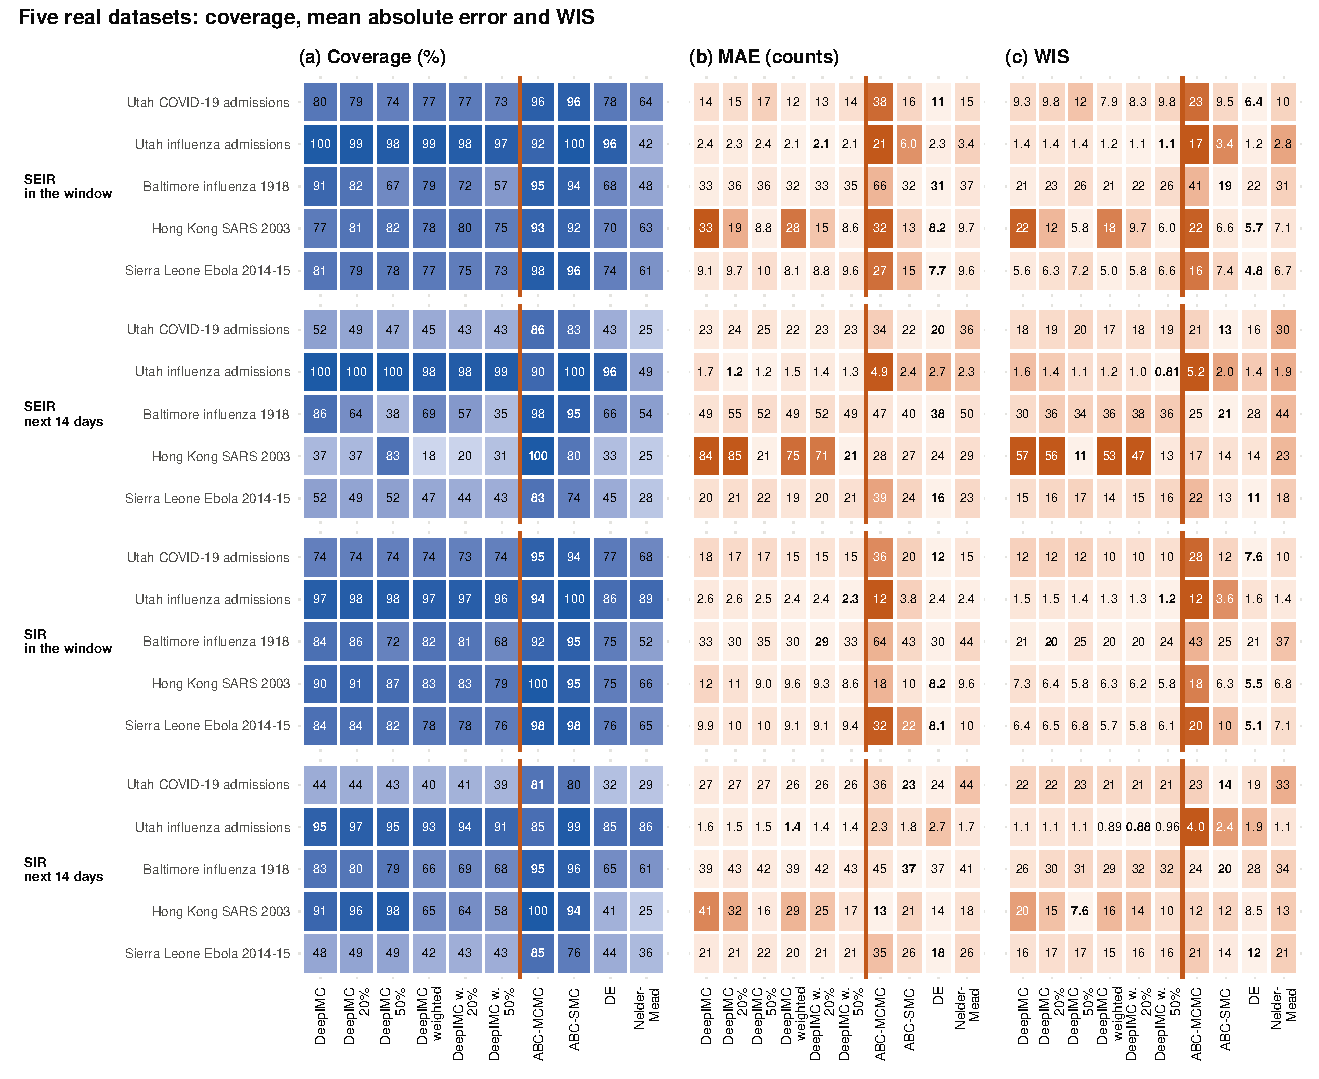
\includegraphics[width=\textwidth]{figures/coverage_mae_real.pdf}
\caption{Real data. (a) Mean coverage of the 95\% band of each method, for each dataset and model, in the
window and in the 14 days after it (bold: closest to 95\%). (b) Mean absolute error of the median
regenerated curve, in daily counts, and (c) mean weighted interval score (bold: lowest). DeepIMC is shown with
the raw counts and with counts smoothed by a Gaussian kernel of 20\% or 50\% of the window length, each without and
with weighting by the data (``w.''); every version is scored against the raw counts.}
\label{fig:heatmap-real}
\end{figure}

\begin{figure}[htbp]
\centering
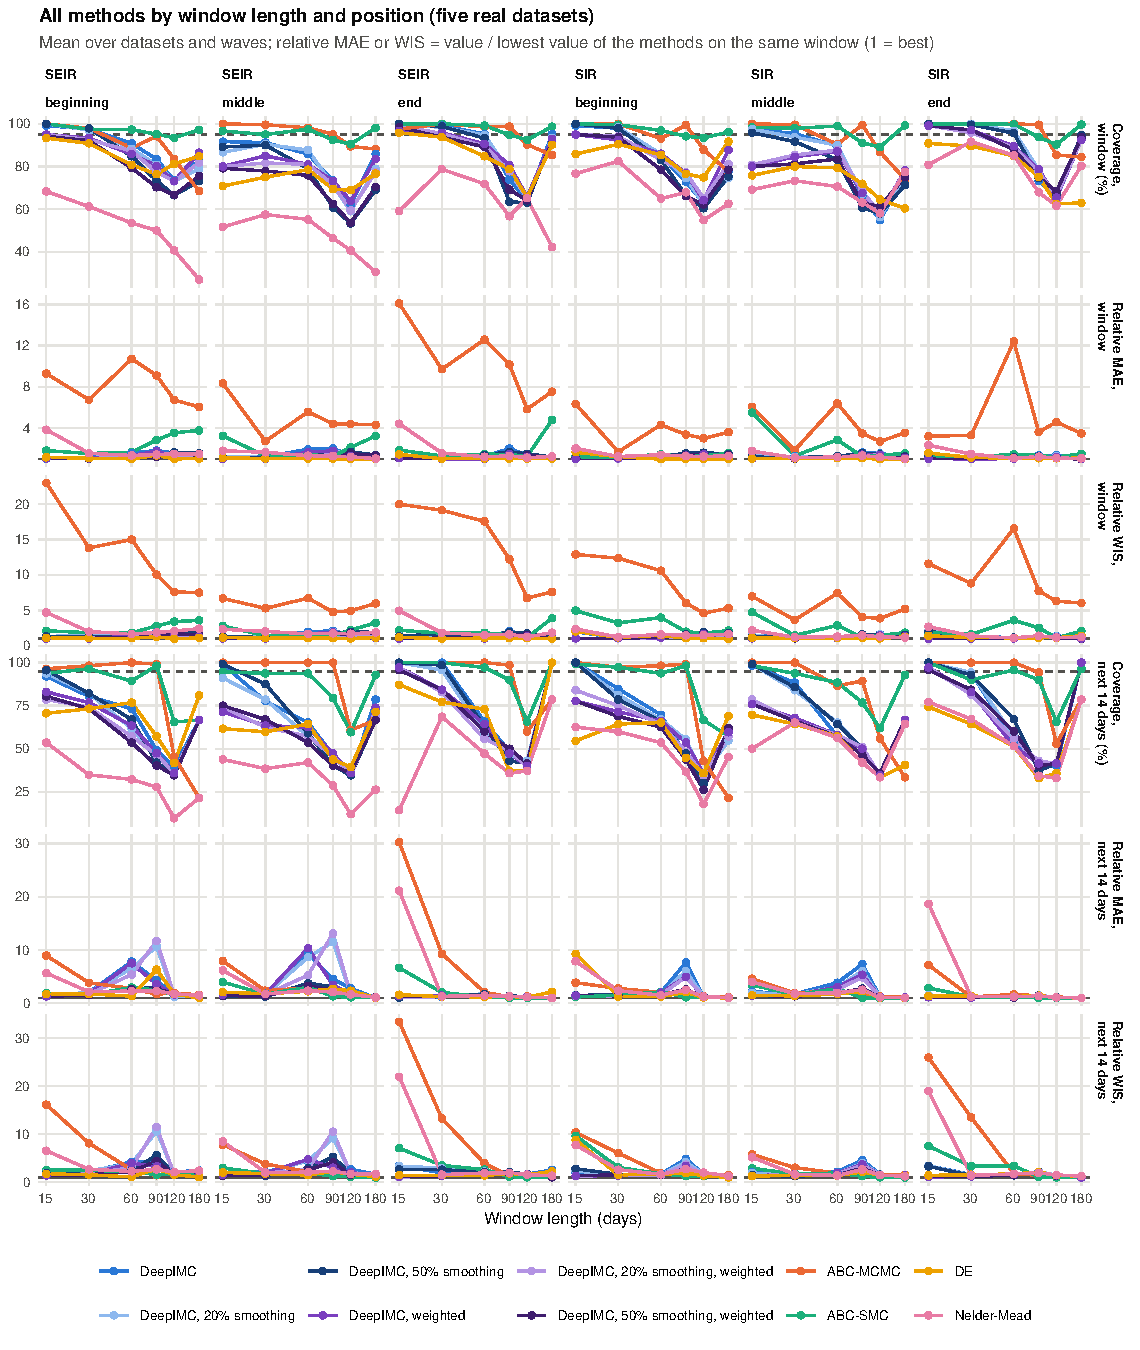
\includegraphics[width=\textwidth]{figures/methods_by_window_real.pdf}
\caption{All methods on the five real datasets, by window length and position: coverage of the observed counts
by the 95\% band and relative MAE of the median regenerated curve (the MAE divided by the lowest MAE of the five
methods on the same window, so that datasets of different size can be averaged; 1 is best), in the window and
in the 14 days after it.}
\label{fig:methods-by-window-real}
\end{figure}

\paragraph{Weighting DeepIMC by the data.} Keeping only the 10\% of DeepIMC's draws whose simulated curves are
closest to the window (Section~\ref{sec:weighting}) brought DeepIMC closer to the data on every dataset except
Baltimore 1918, where it made no difference (Table~\ref{tab:real}); the WIS of the window fell in 86\% of the
windows. Over the five datasets the WIS fell from 8.7 to 7.7 and the MAE from 13.4 to 11.8, below those of ABC-SMC
(8.9 and 15.4), though still above those of differential evolution (6.3 and 9.7). On the influenza admissions the
weighted DeepIMC fitted the data best of all methods (WIS 1.23 against 1.37 for differential evolution), and on
the 15- and 30-day windows of all datasets it was closer to the data than differential evolution (WIS 4.7 and 5.2
against 5.5). Its bands became narrower, and their coverage fell from 86\% to 83\%. Beyond the window the gain was
small (WIS of the next 14 days 15.4 against 14.7): the weighting chooses the draws that reproduce the window, but
it cannot anticipate changes that come after it. Figure~\ref{fig:ratios-real} compares the weighted DeepIMC with
each method in turn.

\paragraph{The fit check.} The weighting also tells whether any of DeepIMC's draws reproduces the window
(Table~\ref{tab:fit-check}). In all but one of the 10,000 simulated windows, the closest draw was within twice the
Poisson noise of the data. On the real data it was not for 4\% of the Utah influenza windows, a third of the COVID-19 windows, 44\% of
the Ebola windows, 62\% of the SARS windows and 71\% of the Baltimore windows. These are the windows where DeepIMC
fell behind differential evolution: over the five datasets, its WIS was a median 1.37 times that of differential
evolution there, against 1.09 times where a draw reproduced the window. Such windows are noisier than the agent-based model's curves
(Baltimore 1918) or have a shape the model cannot produce with constant parameters (the outbreaks brought under
control, SARS and COVID-19). The difference was largest for the COVID-19 admissions (a median WIS ratio of 1.80
against 1.12) and Ebola (1.21 against 0.94). The check needs no knowledge of the truth, so a user can see when DeepIMC's results
should be read with care.

\begin{table}[htbp]
\centering
\caption{Fit check: percentage of windows that no draw of DeepIMC reproduces within twice the Poisson noise
($d_{\min} > 1$, Section~\ref{sec:weighting}), and DeepIMC's WIS divided by that of differential evolution (median
over the windows) for the windows that are reproduced and those that are not.}
\label{tab:fit-check}
\small
\begin{tabular}{lrrrr}
\toprule
 & Windows & Not reproduced (\%) & \multicolumn{2}{c}{DeepIMC WIS / DE WIS} \\
\cmidrule(lr){4-5}
Data &  &  & reproduced & not reproduced \\
\midrule
Simulated (10,000 windows) & 10,000 & 0.0 &  &  \\
Utah COVID-19 admissions & 90 & 33 & 1.12 & 1.80 \\
Utah influenza admissions & 72 & 4 & 1.10 & 0.98 \\
Baltimore influenza 1918 & 24 & 71 & 0.96 & 1.01 \\
Hong Kong SARS 2003 & 24 & 62 & 1.35 & 1.37 \\
Sierra Leone Ebola 2014-15 & 36 & 44 & 0.94 & 1.21 \\
\bottomrule
\end{tabular}

\end{table}

\paragraph{Smoothing.} Smoothing the counts before DeepIMC reads them, with any of the usual kernels (Gaussian,
moving average, Epanechnikov, local-linear or robust; Appendix~\ref{app:smoothing}), helped only where the data jump
and added little to the weighting. The shape of the kernel made almost no difference; heavy smoothing, with a kernel
of 50\% of the window, flattened the real peak of Baltimore 1918 and hurt there and on most other datasets, but it
was the only remedy for the cluster of SARS cases (WIS 5.8, as low as differential evolution). Combined with the
weighting, the best smoother brought the WIS over the five datasets from 7.7 to 7.3, nearly all of it on SARS.

Figure~\ref{fig:real-examples-deepimc} shows the six versions of DeepIMC (raw counts, a 20\% or a 50\% kernel, each
without and with the weighting) on the window around the peak of each dataset, with the smoothed counts that DeepIMC
read. Smoothing changes these counts a great deal (it lowered the peak of the window by a median 33\% with the 20\%
kernel and 44\% with the 50\% kernel), but DeepIMC's estimate of $R_0$ much less: the median change was 0.02 and
0.06, because the network reads $R_0$ mainly from how fast the curve grows and declines, which a kernel keeps, and
because it learned from the agent-based model's own noisy curves. With the weighting, the 20\% kernel lowered the WIS
over the five datasets from 7.7 to 7.4 and the 50\% kernel raised it to 7.9; on SARS they lowered it from 12.4 to 8.0
and 5.9 (differential evolution 5.6), while on Baltimore 1918 the 50\% kernel raised it from 20.7 to 25.2. In the next
14 days, the weighted DeepIMC with the 50\% kernel had the lowest WIS of the DeepIMC versions (13.8, against 14.8 with
the raw counts), still above ABC-SMC (10.4) and differential evolution (11.8).

\begin{figure}[htbp]
\centering
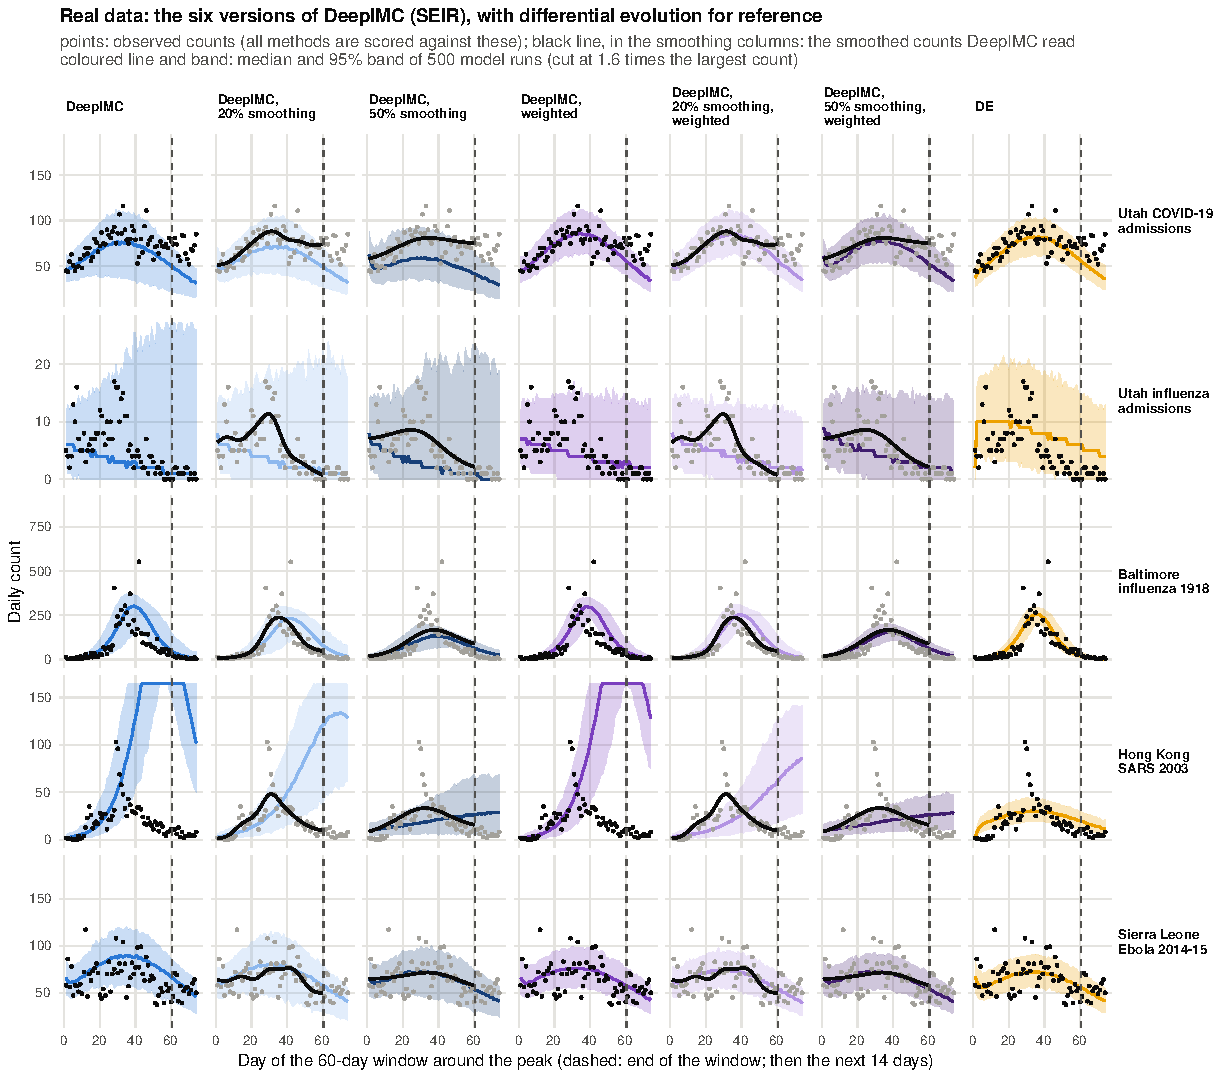
\includegraphics[width=\textwidth]{figures/real_examples_deepimc.pdf}
\caption{Real data: the six versions of DeepIMC (raw counts, and counts smoothed by a Gaussian kernel of 20\% or
50\% of the window length, each without and with weighting by the data) and differential evolution for reference:
SEIR fits to the 60-day window in the middle of each dataset, with the next 14 days (after the dashed line). Points:
observed counts, against which every version is scored (grey in the smoothing columns); black line: the smoothed
counts that DeepIMC read; coloured lines and bands: median and 95\% band of 500 model runs (cut at 1.6 times the
largest observed count). The SIR fits are in Figure~\ref{fig:real-examples-deepimc-sir}.}
\label{fig:real-examples-deepimc}
\end{figure}

\paragraph{Six more outbreaks.} Was the Hong Kong outbreak hard because of SARS, because of clusters of cases, or
because of the Hong Kong data? On six more outbreaks (Appendix~\ref{app:extra}), among them SARS in Canada and two
outbreaks spread largely in hospitals, the weighted DeepIMC came closer to the data than differential evolution on
four and closer than ABC-SMC on five. Over their 114 windows its WIS was 1.20, against 1.39 for differential
evolution and 1.79 for ABC-SMC, and in the next 14 days 3.6, against 6.3 and 3.8. On SARS in Canada the fit check
flagged no window, and DeepIMC was closer to the data than every comparison method. The difficulty in Hong Kong lies
in a single day: the counts rise from 31 to 103 between days 37 and 38 of the outbreak, most likely the outbreak in
the Amoy Gardens housing estate, where more than 300 residents fell ill within days \autocite{yu2004evidence}. On the
Hong Kong windows that end before this day or start after it, the weighted DeepIMC was closer to the data than
differential evolution (WIS 1.42 against 1.57, and 0.67 against 0.77); on the 14 windows that contain it, the fit
check flagged every window and its WIS was 20.5, against 8.9.

\begin{figure}[htbp]
\centering
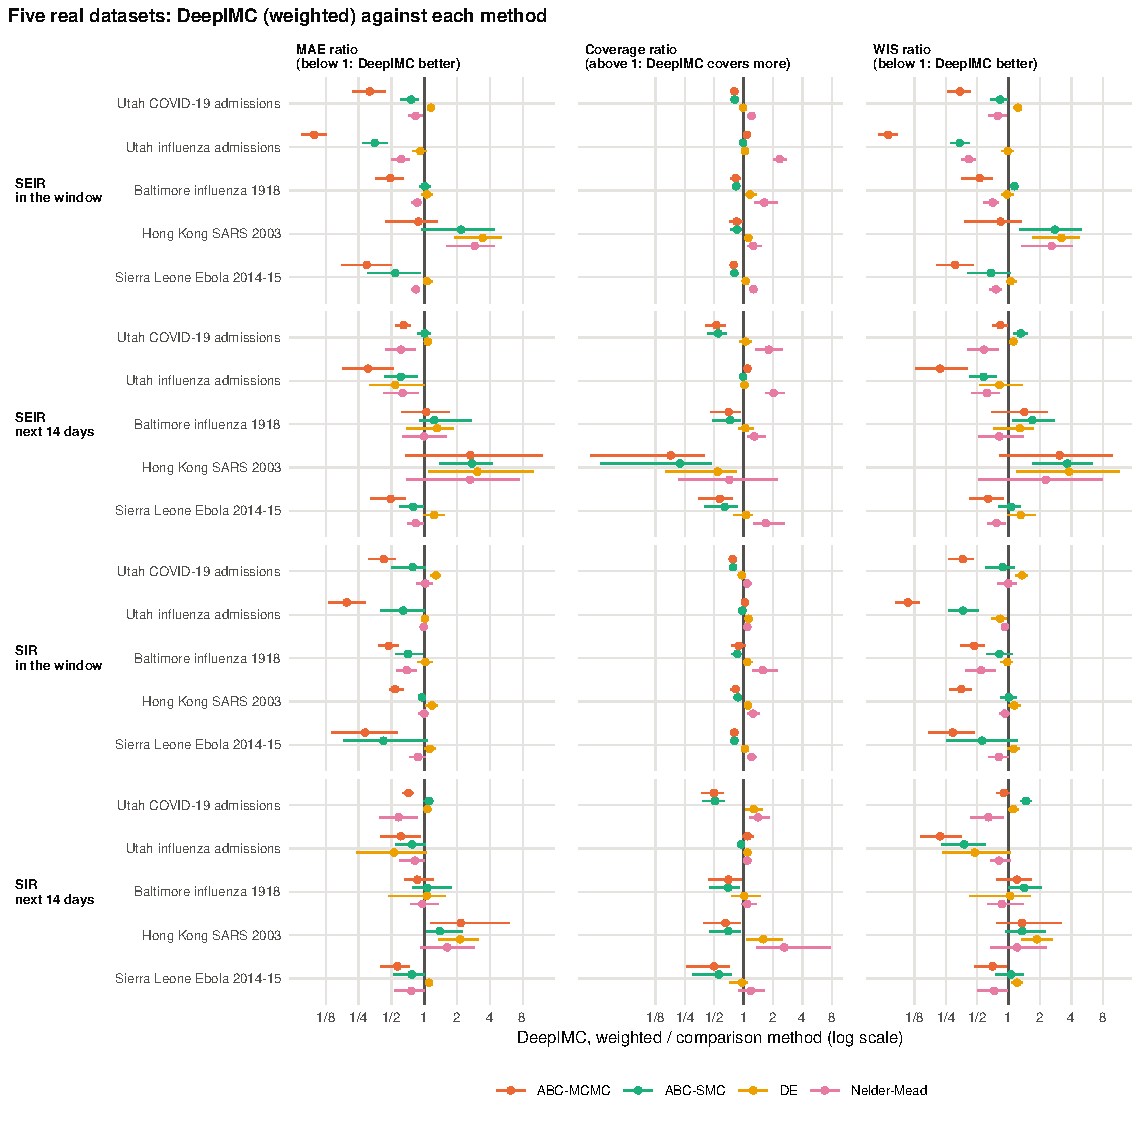
\includegraphics[width=\textwidth]{figures/ratios_real_weighted.pdf}
\caption{Real data: weighted DeepIMC's mean MAE, mean coverage and mean WIS divided by those of each comparison
method on the same windows, for each dataset, in the window and in the next 14 days, with 95\% bootstrap intervals
(log scale). The same comparison for DeepIMC without weighting is in Figure~\ref{fig:ratios-real-auto}, and for the
weighted DeepIMC with a 20\% or a 50\% kernel in Figures~\ref{fig:ratios-real-w20} and~\ref{fig:ratios-real-w50}.}
\label{fig:ratios-real}
\end{figure}

\begin{sidewaysfigure}
\centering
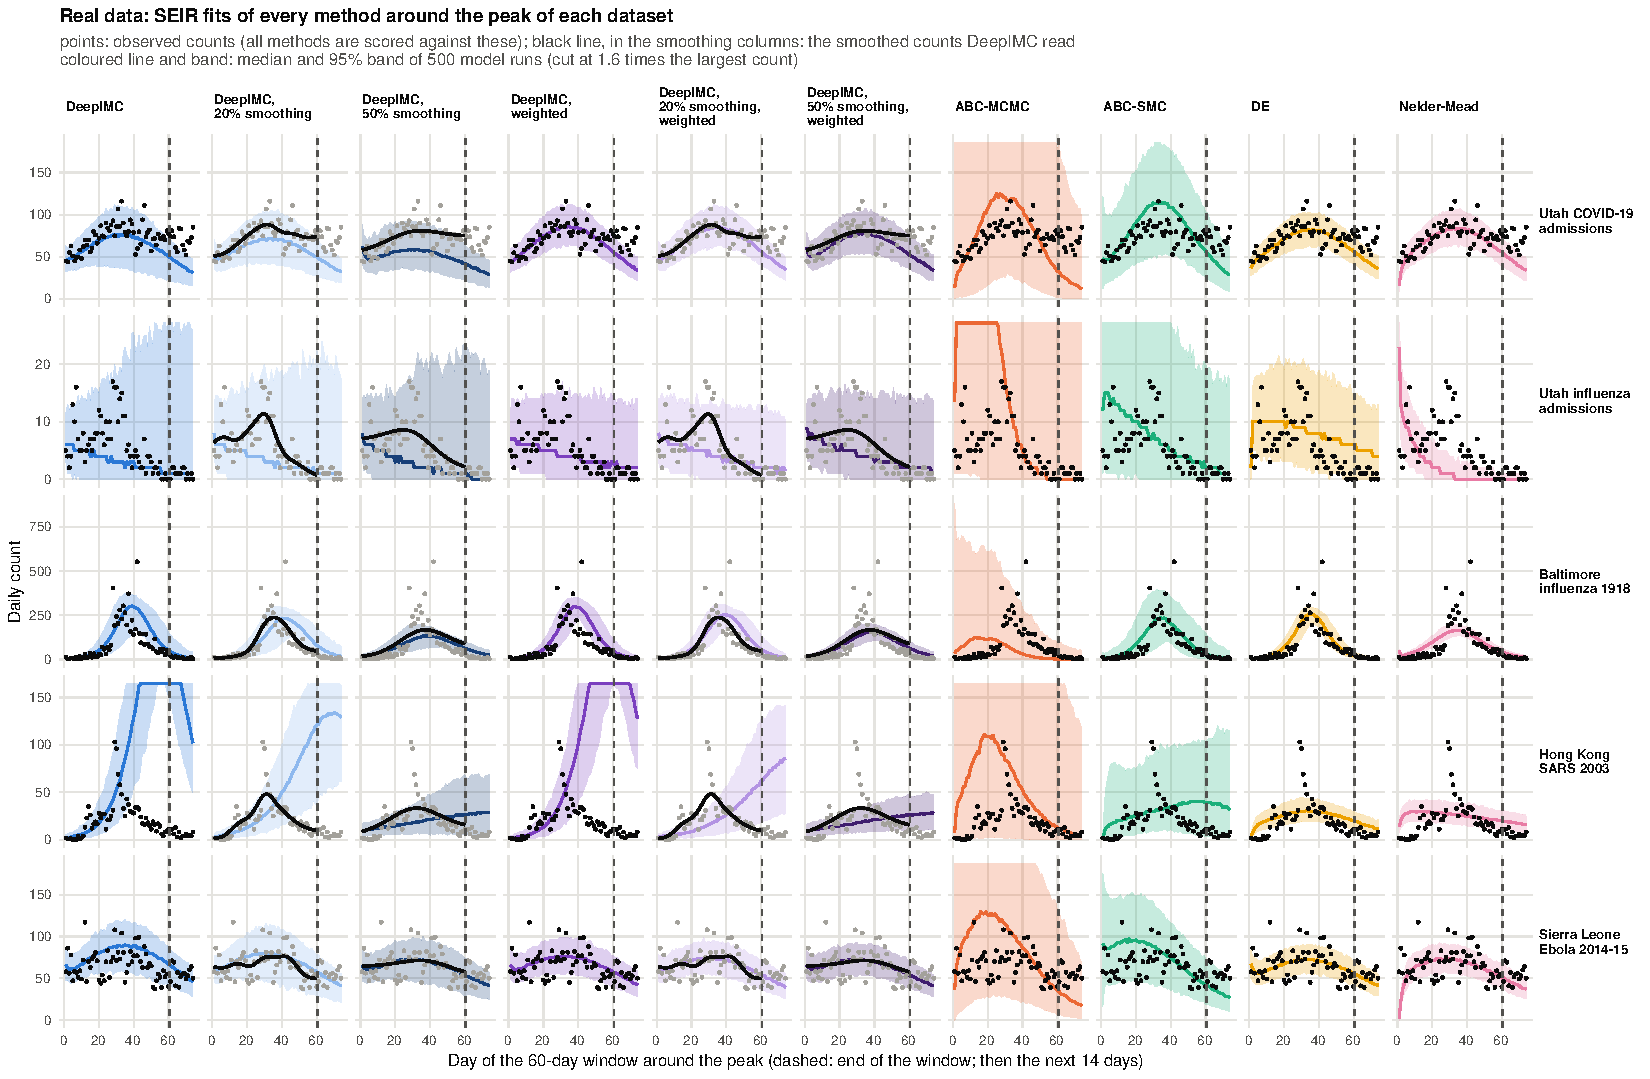
\includegraphics[width=\textheight]{figures/real_examples.pdf}
\caption{Real data: SEIR fits of every method to the 60-day window in the middle of each dataset, with the next
14 days (after the dashed line). DeepIMC is shown in six versions: raw counts, and counts smoothed by a Gaussian
kernel of 20\% or 50\% of the window length, each without and with weighting by the data. Points: observed counts, against which every method is scored (grey in the
columns where DeepIMC read smoothed counts); black line: the smoothed counts DeepIMC read in those columns; coloured
lines and bands: median and 95\% band of 500 model runs from each method's estimates (cut at 1.6 times the largest
observed count). The SIR fits are in Figure~\ref{fig:real-examples-sir}.}
\label{fig:real-examples}
\end{sidewaysfigure}

\subsection{Computing time}\label{sec:res-cost}

The last question is what each method costs. Table~\ref{tab:timing} separates the cost of calibrating a
new window from DeepIMC's one-time cost of training.

\paragraph{Calibrating a window.} On one CPU core, DeepIMC calibrated a window in 0.15 seconds (SEIR) and
0.08 seconds (SIR), and about as fast per window when several windows were processed together. Its first
call in an R session took 9.6 and 6.3 seconds, almost all of it to start Python and load the five
networks; this is paid once per session. The comparison methods took between 3.0 seconds (Nelder--Mead,
SIR) and 588 seconds (differential evolution, SEIR) per window. For SEIR windows, DeepIMC was about 1,300
times faster than ABC-MCMC, 2,300 times faster than ABC-SMC and 3,900 times faster than differential
evolution; it was 65 times faster than Nelder--Mead, the cheapest of the comparison methods.

\paragraph{From a fit to a band.} Turning a fit into a 95\% band with 500 runs of the agent-based model
took 38 (SEIR) and 13 (SIR) seconds per window, far longer than DeepIMC's fit itself. The renewal equation
gave a band in 0.20 and 0.12 seconds.

\paragraph{The one-time cost.} Simulating the 1,000,000 training epidemics took 27 (SEIR) and 13 (SIR)
CPU-hours, and computing DeepIMC's estimates for the 100,000 calibration windows of the $R_0$ range 1.4 and
0.2 hours on one core. Training is the largest part: one SEIR network would need about 86 hours on 16 CPU
cores (27 hours for SIR), which is why we trained on GPUs, where one network took 2.7 to 11.4 hours depending
on the model and the GPU. The simulation time alone equals the cost of calibrating about 170 SEIR windows with
differential evolution or 280 with ABC-SMC; with training on CPUs, the one-time cost equals tens of
thousands of windows. It is paid once, by the developer: the trained networks are shipped with the
package, and its users pay only the cost of a calibration.

\begin{table}[htbp]
\centering
\caption{Computing time on CPUs (one core per method, the same computer for all methods), and the
one-time cost of DeepIMC.}
\label{tab:timing}
\small
\begin{tabular}{lrr}
\toprule
 & SEIR & SIR \\
\midrule
\multicolumn{3}{l}{\textit{Calibrating one window (seconds, one CPU core)}} \\
DeepIMC, first call (starts Python, loads networks) & 9.6 & 6.3 \\
DeepIMC, one window & 0.150 & 0.082 \\
DeepIMC, 10 windows in one pass, per window & 0.127 & 0.084 \\
ABC-MCMC & 194.0 & 84.4 \\
ABC-SMC & 344.4 & 124.9 \\
DE & 588.3 & 163.3 \\
Nelder--Mead & 9.8 & 3.0 \\
\midrule
\multicolumn{3}{l}{\textit{From a fit to a 95\% band (seconds per window)}} \\
500 runs of the agent-based model & 38.3 & 12.7 \\
Renewal equation & 0.203 & 0.123 \\
\midrule
\multicolumn{3}{l}{\textit{One-time cost of DeepIMC (CPU)}} \\
Simulating 1,000,000 training epidemics (CPU-hours) & 27.2 & 13.5 \\
Estimates for 100,000 calibration windows (hours, 1 core) & 1.4 & 0.2 \\
Training one network, 50 epochs (hours, 16 cores, estimated) & 85.7 & 26.8 \\
\midrule
\multicolumn{3}{l}{\textit{For reference: training as done, on GPUs}} \\
Training one network, 50 epochs (hours, one GPU) & 5.8--11.4 & 2.7--9.9 \\
\bottomrule
\end{tabular}

\end{table}

% =============================================================================
\section{Discussion}\label{sec:discussion}

We introduced DeepIMC, a neural network that maps a window of daily new infections of any length, from
any part of an epidemic, to the basic reproduction number and the current state of an agent-based SEIR or
SIR epidemic. On 10,000 simulated test windows of 15 to 365 days, where the truth is known, it estimated
$R_0$ about three times more accurately than four standard calibration methods used with their default
settings, and more accurately in every group of window length and position. Its ranges
for $R_0$ had close to nominal coverage while being far narrower than those of ABC; it recovered the state of
the epidemic, and the number of infectious people that no method observes, better than every other method;
and it calibrated a window in a fraction of a second on one CPU core. Scoring the curves by a single number
that combines accuracy and coverage, the weighted interval score, or by the cumulative number of infections,
did not change these conclusions. On real data the comparison was closer, and depended on how closely each
dataset matched the model.

\subsection{What the curve can and cannot tell}

The transmission probability and the contact rate cannot be separated from a curve of daily
infections, by DeepIMC or by any other method: their errors equal those of a guess that knows $R_0$
exactly, because only their product shapes the epidemic. This does not limit the use of a calibrated
model for prediction, which depends on $R_0$ and the current state; but estimating $p_{tran}$ and
$c_{rate}$ separately requires additional information, such as contact rates from a contact survey.

\subsection{Why DeepIMC is more accurate}

At the beginning of an epidemic, the growth of the curve reveals $R_0$ almost directly, and differential
evolution came closest to DeepIMC. In the middle and at the end of an epidemic, a method must also find
how many people are already infected or immune, and many combinations of $R_0$ and starting state produce
similar curves. The comparison methods search this space by trial and error, over thousands of stochastic
simulations, for every window; DeepIMC has learned from a million simulated epidemics which combinations are
likely, and this is where its advantage was largest.

The comparison methods failed in different ways. Differential evolution matched the observed curve as closely
as DeepIMC, because it fits each window directly, but its single estimate could not express how uncertain the
starting state is, and its estimate of the unobserved number of infectious people was twice as far from the
truth. ABC-MCMC, with its tolerance set from 200 simulations from the prior, stayed close to the prior: its
estimates were pulled towards the middle of the range and its ranges covered most of it. ABC-SMC was the most
accurate comparison method for SEIR windows but still underestimated many large values of $R_0$. Nelder--Mead
was the weakest method on the curves: with a fixed-seed agent-based model the fit is flat and irregular, so its
stopping rule is met after about 100 runs, often far from the best values.

\subsection{Ease of use}

DeepIMC needs only the daily counts and the known values. Each comparison method required choices
before it could be used: ranges for $R_0$ and for the starting state, how to parameterize them, the
number of model runs, tolerances and, for ABC, the summary statistics and their scaling. Even with
default settings, ABC-SMC failed on most SEIR windows until its limits were raised. These choices
are made once, by the developer, when DeepIMC is trained; users of the trained models do not face them.

\subsection{Real data and the choice of data}

DeepIMC was trained on noise-free epidemics, in which every new infection is counted, in a closed
population with constant parameters. Real data depart from these assumptions in three ways: only a
fraction of infections is recorded, the recorded counts depend on testing and reporting, and the course
of an epidemic changes with behaviour and interventions. The choice of data therefore matters. Counts by
date of symptom onset and hospital admissions by date of admission follow new infections more closely
than cases by date of report, which follow the reporting week and the availability of tests. On the
datasets closest to the model's assumptions---influenza waves recorded by admission or onset, and the
Ebola outbreak---DeepIMC fitted the data almost as closely as the best comparison method, in a fraction of
a second, and on short windows of any dataset it was as close as the best comparison method. On outbreaks
that were brought under control, such as SARS in Hong Kong, no method with constant parameters can follow the
decline, and DeepIMC, whose bands are narrower, was penalized most.

\paragraph{Using the data twice.} DeepIMC is fast because it does not search: it maps the curve to the estimates it
learned. When a real curve is unlike the simulated ones, that mapping has nothing to correct it. Weighting its
parameter draws by how well they reproduce the window restores this missing step at a small cost, without
retraining the networks or changing the model: it brought DeepIMC closer to the data on four of the five
datasets and closer than differential evolution on short windows, and on simulated data it improved the starting
state and the curves. Its by-product, the fit check, is perhaps as useful: it tells the user, without knowing
the truth, when no plausible parameter set of the model reproduces the data, which is when DeepIMC fell behind the
methods that fit each window directly. Smoothing the counts was a weaker remedy, whatever the kernel. It helped
where the data jump, as with the cluster of SARS cases in Hong Kong, and added a little to the weighting, but a
kernel whose width is a fixed fraction of the window smooths long windows over weeks and flattens real peaks, as
in Baltimore 1918. The SARS cluster reflects a
superspreading event that a homogeneous agent-based model does not represent \autocite{yu2004evidence}; smoothing it
treats that event as noise, which should be stated whenever it is done. Six more outbreaks, SARS in Canada among
them, showed that the difficulty belongs to this one cluster rather than to SARS or to real outbreaks in general:
on them the weighted DeepIMC was closer to the data than differential evolution (Appendix~\ref{app:extra}). The comparison methods were not given smoothed or weighted
data, because neither is part of how they are used.

\subsection{Computational efficiency}

Because DeepIMC calibrates a window in a fraction of a second on an ordinary CPU, it can be used where the
standard methods are impractical: for many locations at once, every day of an ongoing outbreak as new
data arrive, or inside a larger analysis that calibrates thousands of windows, such as the evaluation in
this paper. The cost is moved to training, which in practice needs a GPU and is paid once for each model
structure and range of parameters. For a model that will be calibrated only a few times, a standard
method is cheaper; for a model that is calibrated repeatedly, as in surveillance or by the many users of
a shipped model, the one-time cost is soon recovered. Once the calibration takes a fraction of a second,
the slowest step of a prediction is the simulation of the band.

The renewal equation reduces that step to a fraction of a second (Appendix~\ref{sec:res-renewal}): started from
DeepIMC's estimated state, it
gave nearly the same curves of new infections as 500 model runs, about 190 times faster, at the price of bands for the
number currently infectious that are too narrow.
\subsection{Limitations}

The models assume homogeneous mixing, parameters that are constant within a window, and a known
population size, recovery rate and latent period. Real population sizes must be mapped to the trained
range, and the reported fraction of infections cannot be separated from the population size. The trained
ranges of Table~\ref{tab:priors} bound the epidemics the shipped models can calibrate: the shortest
infectious period is 4 days, longer than that of influenza, so influenza is represented with a longer
generation interval than observed. Other settings require new training data and retraining, which the
software supports. Finally, the $R_0$ ranges are calibrated empirically on simulated windows rather than
derived from a posterior distribution.

\subsection{Future work}

Training DeepIMC on simulated reported data---with a reported fraction of infections, a weekly reporting
pattern and extra noise---would let it read case reports directly. Parameters that change over time,
other contact structures such as networks, and models with hospitalization are natural extensions; the
same training code applies to any model that can be simulated.

% =============================================================================
\section{Conclusions}

Calibrating agent-based models is computationally demanding and requires many choices from the user.
DeepIMC reverses the usual approach: it learns, once, the inverse mapping from epidemic curves to the
quantities that generated them, using data simulated from the model itself. For agent-based SEIR and SIR
models, it estimates $R_0$ and the current state of an epidemic from a window of any length and position,
reproduces the epidemic those estimates imply, and answers in a fraction of a second on an ordinary CPU,
with no settings to choose. How well it does on real data depends on how closely the data resemble the
simulations it was trained on, which makes the choice of data---onset dates and admissions rather than
reported cases---as important as the choice of method.

% =============================================================================
\section{Software availability}

The R package \texttt{epiworldRcalibrate} provides:
\begin{itemize}
\item the trained SEIR and SIR calibrators: \texttt{window\_calibrator()} and \texttt{calibrate()};
\item the four comparison methods, set up as in this paper: \texttt{window\_baselines()}, with
\texttt{epidemic\_summary()} for the summary statistics of the ABC methods;
\item predictions by model simulation or the renewal equation: \texttt{predict\_cases()};
\item the evaluation scores: \texttt{coverage()}, \texttt{interval\_score()} and \texttt{score\_band()};
\item the comparison of methods on many windows: \texttt{compare\_methods()};
\item simulation of training data, tuning and training of new calibrators:
  \texttt{simulate\_window\_data()}, \texttt{tune\_window\_calibrator()} and
  \texttt{train\_window\_calibrator()}.
\end{itemize}
All code needed to reproduce the results is available at: repository link removed for double-blind review.

\section*{Acknowledgments}
Acknowledgments removed for double-blind review.

\printbibliography

% =============================================================================
\appendix

\section{Simulation details}\label{sec:sim-parameters}

Epidemics were simulated with \texttt{ModelSEIRCONN} and \texttt{ModelSIRCONN} of \textbf{epiworldR} for
365 days with the distributions of Table~\ref{tab:priors}. A new epidemic starts with the drawn share of
the population exposed (SEIR) or infectious (SIR) and nobody recovered. The daily count is the number of
transitions from exposed to infectious (SEIR) or from susceptible to infectious (SIR); the shares in each
state are recorded at the start of each day, so the state at the start of a window is the state at the
start of its first day. Separate sets were simulated for training (1,000,000 epidemics per model, 80\% for
training and 20\% for validation), for the calibration windows of the $R_0$ range (100,000), for the test
of DeepIMC by window length (1,000) and for the comparison with the other methods (10,000 in all).

\section{Network and training details}\label{app:training}

\begin{table}[htbp]
\centering
\caption{Settings of the two DeepIMC models. The search space of the hyperparameter search is given in
brackets.}
\label{tab:hyper}
\small
\resizebox{\textwidth}{!}{%
\begin{tabular}{lll}
\toprule
Setting & SEIR & SIR \\
\midrule
BiLSTM layers [1--3] & 3 & 2 \\
Hidden units per direction [64, 128, 160, 256] & 128 & 64 \\
Dropout between layers [0--0.5] & 0.13 & 0.28 \\
Initial learning rate [$10^{-4}$--$10^{-3}$, log scale] & $7.16\times10^{-4}$ & $7.94\times10^{-4}$ \\
Batch size [32, 64, 128, 256] & 32 & 32 \\
Learning-rate schedule & cosine, to 1\% over 50 epochs & same \\
Gradient-norm clipping & 1 & 1 \\
Dense layer & 64 units, ReLU & same \\
Output activations & sigmoid ($p_{tran}$, shares), softplus ($R_0$) & same \\
Networks averaged & 5 & 5 \\
\bottomrule
\end{tabular}}
\end{table}

The hyperparameter search used Optuna's tree-structured Parzen estimator with a median pruner (trials worse
than the median of earlier trials after 5 epochs were stopped). Each trial trained one network for 20 epochs
on 100,000 training epidemics (windows of 30 to 365 days, the range of the networks at that stage; the final
networks for 15 to 365 days use the same settings) and was scored by the validation mean squared error, half for
$R_0$ and half
for the state shares. The best settings (Table~\ref{tab:hyper}) improved the validation score by 3\% (SEIR)
and 5\% (SIR) over the settings of an earlier model.

Table~\ref{tab:versions} compares the versions of the networks on the same test windows. The first three were
trained on windows of 30 to 365 days: \emph{Current} uses the settings of the earlier model, 300,000 training
epidemics and 100 epochs with a constant learning rate; \emph{Tuned} uses the settings of
Table~\ref{tab:hyper}, otherwise as Current; \emph{Final} uses the tuned settings, 1,000,000 epidemics and the
cosine learning-rate schedule over 50 epochs. Tuning alone changed the test errors little; more training data and the
decreasing learning rate reduced the $R_0$ error further. As expected, no version improved $p_{tran}$ or
$c_{rate}$, which the curves do not reveal. The networks used in this paper were then trained again with the final
settings for windows of 15 to 365 days instead of 30 to 365; these are the networks used throughout the paper and
shipped with the package (``Final, 15--365'' in Table~\ref{tab:versions}). On the windows that both versions can
read they perform alike: over all test windows of 30 to 365 days their $R_0$ MAE was 0.216 (SEIR) and 0.186 (SIR),
against 0.218 and 0.189 for the version trained on 30 to 365 days, and on 15-day windows, which only they can read,
it was 0.73 and 0.47.

\begin{table}[htbp]
\centering
\caption{Mean absolute error of $R_0$, $p_{tran}$ and $c_{rate}$ of the versions of the networks (5 networks
each) on the same test windows: 61-day windows from the beginning of the test epidemics, all test windows of 30 to
365 days (at the beginning, middle and end), which every version can read, and, for the final networks trained on
windows of 15 to 365 days (the networks of this paper), 15-day windows.}
\label{tab:versions}
\small
\begin{tabular}{lllrrrrrrr}
\toprule
 &  & Trained & \multicolumn{3}{c}{61-day windows from the beginning} & \multicolumn{3}{c}{Windows of 30--365 days} & 15 days \\
\cmidrule(lr){4-6}\cmidrule(lr){7-9}\cmidrule(lr){10-10}
Model & Version & on (days) & $R_0$ & $p_{tran}$ & $c_{rate}$ & $R_0$ & $p_{tran}$ & $c_{rate}$ & $R_0$ \\
\midrule
SEIR & Current & 30--365 & 0.121 & 0.0145 & 2.58 & 0.223 & 0.0141 & 2.56 & -- \\
 & Tuned & 30--365 & 0.118 & 0.0147 & 2.60 & 0.225 & 0.0141 & 2.57 & -- \\
 & Final & 30--365 & 0.107 & 0.0145 & 2.59 & 0.218 & 0.0141 & 2.57 & -- \\
 & Final & 15--365 & 0.109 & 0.0145 & 2.58 & 0.216 & 0.0141 & 2.56 & 0.734 \\
\midrule
SIR & Current & 30--365 & 0.109 & 0.0483 & 1.06 & 0.192 & 0.0524 & 1.05 & -- \\
 & Tuned & 30--365 & 0.106 & 0.0490 & 1.08 & 0.195 & 0.0532 & 1.07 & -- \\
 & Final & 30--365 & 0.098 & 0.0486 & 1.07 & 0.189 & 0.0527 & 1.06 & -- \\
 & Final & 15--365 & 0.101 & 0.0489 & 1.07 & 0.186 & 0.0528 & 1.06 & 0.466 \\
\bottomrule
\end{tabular}

\end{table}

\section{Comparison methods}\label{app:baselines}

All four methods search $\vartheta = (R_0, \log_{10} e_0, \log_{10} i_0, \log_{10} r_0)$ for SEIR and
$(R_0, \log_{10} i_0, \log_{10} r_0)$ for SIR, where $e_0$, $i_0$ and $r_0$ are the shares exposed,
infectious and recovered on the first day of the window, within $R_0\in[0.8, 5]$,
$\log_{10} e_0, \log_{10} i_0 \in [-4, \log_{10} 0.4]$ and $\log_{10} r_0 \in [-4, \log_{10} 0.95]$. If the
shares add up to more than 0.95 they are scaled down to 0.95. The contact rate is fixed at the middle of its
training range (10 for SEIR, 3 for SIR) and $p_{tran} = R_0\, p_{recov}/c_{rate}$. For a candidate
$\vartheta$, the model is run for the length of the window from the candidate state, and its daily new
infectious people $\hat y_t(\vartheta)$ are compared with the observed counts $y_t$: by
$\sum_t (y_t - \hat y_t(\vartheta))^2$ for DE and Nelder--Mead, and through summary statistics for the ABC
methods.

\paragraph{Summary statistics.} For a curve $x_1,\dots,x_T$: $\log(1+\bar x)$, $\log(1+\max_t x_t)$,
$\log(1+\min_t x_t)$, the day of the maximum of the centred 7-day average, $\log(1+\cdot)$ of the mean of
the first and of the last 7 days, the first days on which the cumulative count reaches 25\%, 50\% and 75\%
of $\sum_t x_t$, and the least-squares slopes of $\log(1+x_t)$ against $t$ over the first and the last 14
days (function \texttt{epidemic\_summary()} of the package). With $s(\cdot)$ the vector of statistics and
$\sigma_k$ the median absolute deviation of statistic $k$ over simulations from the prior, the distance is
$d = \big(\frac1K\sum_k [(s_k(\hat y)-s_k(y))/\sigma_k]^2\big)^{1/2}$.

\paragraph{ABC-MCMC.} 200 simulations from the prior give $\sigma_k$ and the tolerance $\varepsilon$, the 5\%
quantile of their distances; Gaussian random-walk proposals with standard deviation 8\% of each range,
uniform prior on the box, Gaussian kernel $\exp(-d^2/2\varepsilon^2)$, starting at the middle of the box;
3,000 steps, the last 1,500 kept; estimates are posterior medians and the $R_0$ range the 2.5\% and 97.5\%
posterior quantiles.

\paragraph{ABC-SMC.} 200 particles over 6 generations; the first generation, drawn from the prior, gives
$\sigma_k$; each tolerance is the median distance of the previous generation; perturbation by a
multivariate normal kernel with twice the weighted covariance of the particles; at most 30,000 model runs
and 20,000 attempts per generation.

\paragraph{DE.} \texttt{DEoptim} with strategy 2 (DE/local-to-best/1/bin), population $10 \times$ the number
of unknowns, $F = 0.8$, $CR = 0.5$, 200 generations.

\paragraph{Nelder--Mead.} \texttt{stats::optim} with its default settings (relative tolerance
$\approx 1.5\times10^{-8}$, at most 500 function evaluations), started at the middle of the box; candidates
outside the box receive an infinite fit.

\section{ABC on the whole curve or on summary statistics}\label{app:abc-sensitivity}

The ABC methods were also run comparing the whole curve day by day (root mean squared error, with
ABC-MCMC's tolerance $0.30\times$ the root mean square of the observed counts) on 216 windows of the simulated
test of windows of 15 to 365 days (108 per model, 36 at the beginning, middle and end of the epidemic).
Table~\ref{tab:abc-sensitivity} compares the two versions on the same windows; every fit finished. For ABC-SMC the
summary statistics gave the better estimates: its $R_0$ MAE was 0.66 (SEIR) and 0.49 (SIR), against 0.78 and
0.73 on the whole curve, and its starting-state error was lower. Comparing the whole curve fitted the observed
curve more closely (MAE 6.2 against 8.7 for SEIR and 13.4 against 18.4 for SIR), as expected of a distance that
compares the curve day by day. For ABC-MCMC the whole curve gave the better $R_0$ for SEIR (0.74 against 0.86)
and about the same for SIR (0.77 against 0.75), and a closer fit to the curve; on summary statistics its fixed
tolerance, set from 200 prior simulations, was loose. The paper uses summary statistics for both, which gave
ABC-SMC, the stronger of the two, its best estimates of $R_0$.

\begin{table}[htbp]
\centering
\caption{ABC on the whole curve or on summary statistics, on the same 216 windows of the simulated test of windows
of 15 to 365 days: fits finished, $R_0$ mean absolute error, starting-state error (percentage points), coverage
and MAE of the true daily new infections in the window, and seconds per window (during the evaluation, on shared
computers).}
\label{tab:abc-sensitivity}
\small
\resizebox{\textwidth}{!}{\begin{tabular}{lllrrrrrr}
\toprule
Model & Method & Compares & Finished & $R_0$ MAE & State error & Coverage (\%) & MAE & Seconds \\
\midrule
SEIR & ABC-MCMC & whole curve & 108 of 108 & 0.74 & 8.4 & 99.3 & 10.5 & 102 \\
 & ABC-MCMC & summary statistics & 108 of 108 & 0.86 & 10.8 & 98.5 & 20.0 & 98 \\
 & ABC-SMC & whole curve & 108 of 108 & 0.78 & 7.6 & 99.2 & 6.2 & 270 \\
 & ABC-SMC & summary statistics & 108 of 108 & 0.66 & 5.5 & 99.7 & 8.7 & 202 \\
\midrule
SIR & ABC-MCMC & whole curve & 108 of 108 & 0.77 & 7.3 & 99.0 & 22.6 & 51 \\
 & ABC-MCMC & summary statistics & 108 of 108 & 0.75 & 13.3 & 98.5 & 32.8 & 48 \\
 & ABC-SMC & whole curve & 108 of 108 & 0.73 & 8.6 & 98.5 & 13.4 & 89 \\
 & ABC-SMC & summary statistics & 108 of 108 & 0.49 & 6.4 & 99.3 & 18.4 & 73 \\
\bottomrule
\end{tabular}
}
\end{table}

\section{Real data: SIR fits}\label{app:real-sir}

\begin{sidewaysfigure}
\centering
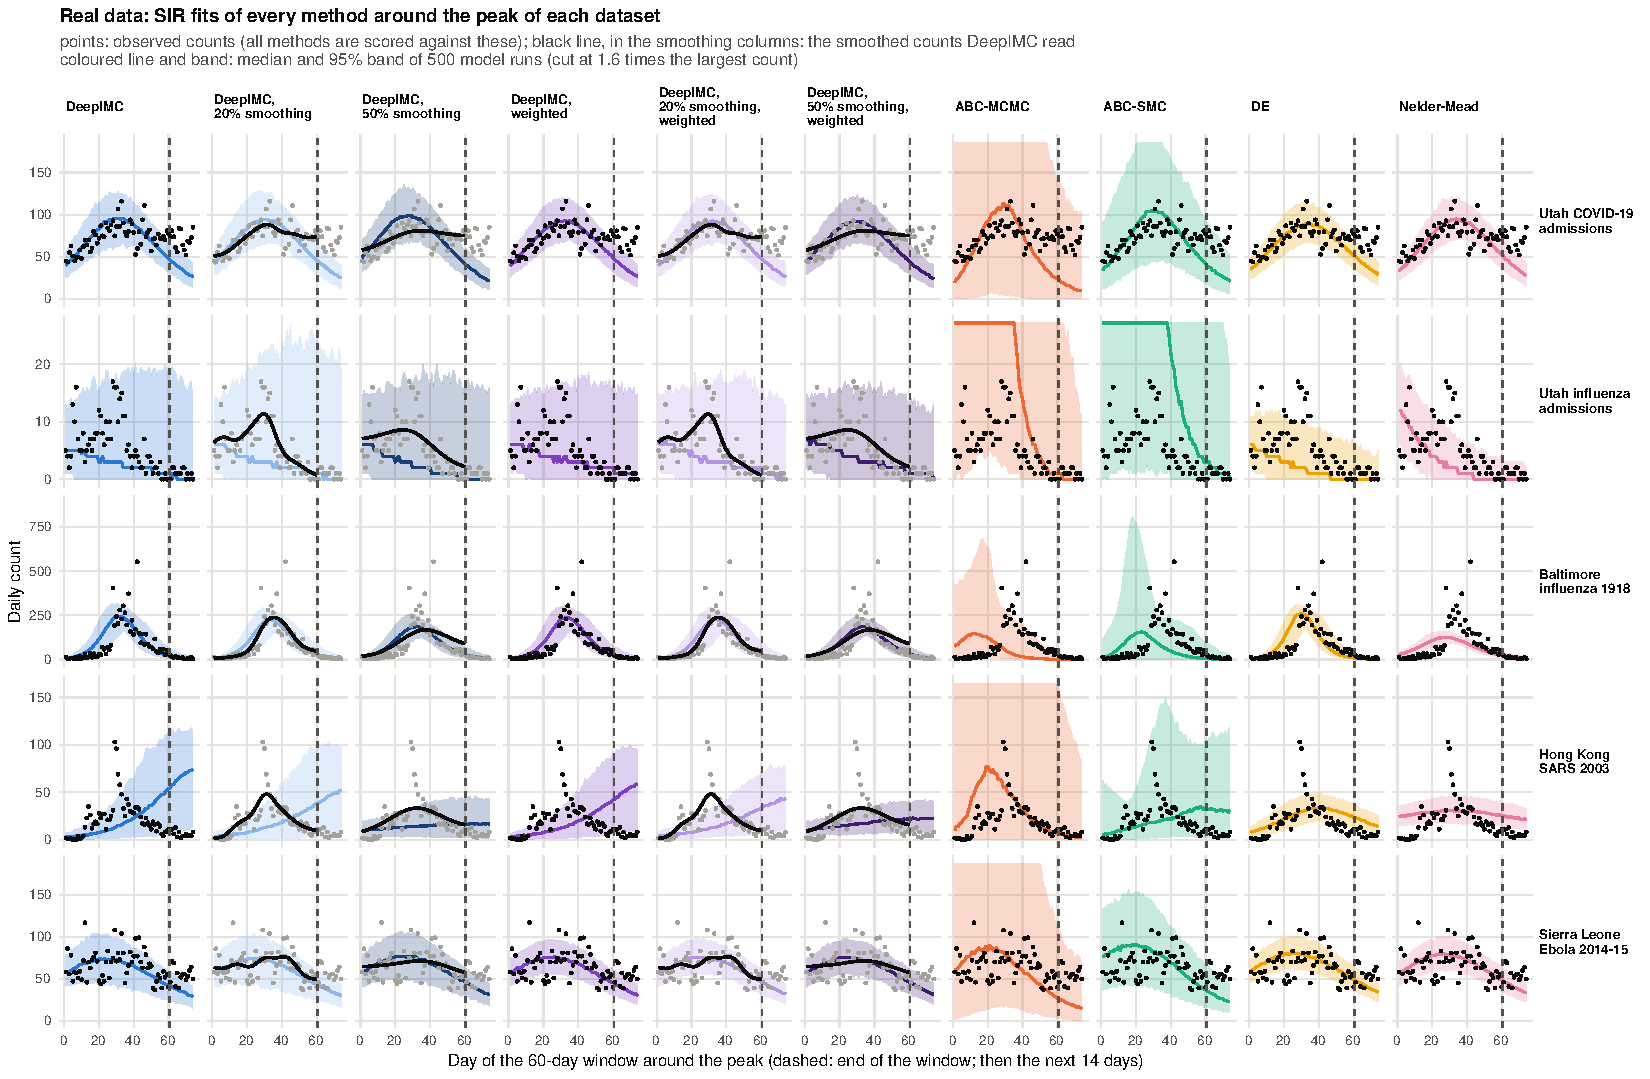
\includegraphics[width=\textheight]{figures/real_examples_sir.pdf}
\caption{Real data: SIR fits of every method to the 60-day window in the middle of each dataset, as in
Figure~\ref{fig:real-examples}.}
\label{fig:real-examples-sir}
\end{sidewaysfigure}

\section{Supplementary results: smoothing the real counts for DeepIMC}\label{app:smoothing}

DeepIMC was given the raw counts and eleven smoothed versions of them, and each version was used both alone and
with the weighting of Section~\ref{sec:weighting}; every version was scored against the raw counts. The smoothers
cover the usual kernels and smoothing methods:
\begin{itemize}[leftmargin=*]
\item a Gaussian kernel (Nadaraya--Watson smoothing) whose bandwidth is 20\% or 50\% of the window length, so that
the amount of smoothing grows with the window (a standard deviation of about 1 or 3 days for a 15-day window, 13
or 33 days for a 180-day window), or whose standard deviation is fixed at 2.5 days;
\item a centred 7-day moving average (a box kernel), the usual smoother of epidemic counts;
\item an Epanechnikov kernel with the same standard deviation as the 2.5-day Gaussian kernel;
\item local-linear smoothing (lowess, with a tricube kernel and a straight line fitted around each day) with a span
of 20\% or 50\% of the window, which follows growth and decline better than a kernel average, also at the ends
of the window, and its robust version, which down-weights outlying days;
\item a 7-day running median followed by the 2.5-day Gaussian kernel, which removes isolated bursts;
\item an automatic rule that applies the running median and the kernel only when a window is noisier than the
agent-based model, that is when the variance of its counts around a centred 7-day mean exceeds twice that mean
(the model's own curves give about 0.9).
\end{itemize}

Table~\ref{tab:real-smoothing} gives the results. The shape of the kernel mattered little: with the same width,
the Gaussian kernel, the moving average, the Epanechnikov kernel and local-linear smoothing gave a WIS between 8.5
and 8.6, against 8.7 for the raw counts. The width mattered more: light smoothing (about 2 to 5 days, or 20\% of the
window) helped a little, while heavy smoothing (50\% of the window) flattened real peaks and hurt, most for
local-linear smoothing (WIS 9.5) and on Baltimore 1918. The weighting lowered the WIS of every version by about
one point (11--12\%). With it, the best versions were the automatic rule (7.32), the Gaussian kernel of 20\% (7.37)
and the running median (7.42), against 7.67 for the weighted raw counts; nearly all of this difference came from
the SARS outbreak (8.9 against 12.4), where only heavy smoothing spread the cluster of cases (5.9 with the 50\%
Gaussian kernel, which hurt on every other dataset).

\begin{table}[htbp]
\centering
\caption{Real data: DeepIMC with the raw counts and eleven smoothed versions of them, each without (not w.) and
with weighting by the data: WIS and coverage (\%) of the observed counts in the window over the five datasets (both
models), and the weighted version's WIS for each dataset; ABC-SMC and DE for comparison. Bold: lowest WIS.}
\label{tab:real-smoothing}
\small
\resizebox{\textwidth}{!}{\begin{tabular}{lrrrrrrrrr}
\toprule
 & \multicolumn{2}{c}{WIS} & \multicolumn{2}{c}{Coverage (\%)} & \multicolumn{5}{c}{WIS weighted, by dataset} \\
\cmidrule(lr){2-3}\cmidrule(lr){4-5}\cmidrule(lr){6-10}
DeepIMC reads & not w. & weighted & not w. & weighted & COVID-19 & Influenza & Baltimore & SARS & Ebola \\
\midrule
Raw counts & 8.68 & 7.67 & 85.6 & 83.2 & 9.03 & 1.23 & 20.70 & 12.35 & 5.37 \\
Gaussian kernel, 20\% & 8.32 & 7.37 & 85.4 & 82.6 & 9.19 & 1.21 & 20.84 & 7.95 & 5.79 \\
Gaussian kernel, 50\% & 8.90 & 7.93 & 82.4 & 79.5 & 9.91 & \textbf{1.18} & 25.20 & \textbf{5.90} & 6.34 \\
Gaussian kernel, 2.5 days & 8.53 & 7.54 & 85.6 & 83.2 & 9.06 & 1.22 & 21.03 & 10.51 & 5.43 \\
7-day moving average & 8.58 & 7.58 & 85.4 & 83.1 & 9.05 & 1.23 & 21.01 & 10.88 & 5.44 \\
Epanechnikov kernel & 8.48 & 7.57 & 85.6 & 83.3 & 9.07 & 1.23 & 20.98 & 10.73 & 5.48 \\
Loess, 20\% & 8.55 & 7.55 & 85.7 & 83.2 & 9.11 & 1.25 & 20.79 & 10.54 & 5.39 \\
Loess, 50\% & 9.54 & 8.45 & 84.8 & 82.3 & 8.93 & 1.26 & 29.72 & 11.26 & 5.59 \\
Robust lowess, 20\% & 8.44 & 7.45 & 85.3 & 82.8 & 9.08 & 1.27 & 20.68 & 9.61 & 5.43 \\
Robust lowess, 50\% & 8.98 & 7.88 & 84.6 & 82.5 & \textbf{8.89} & 1.29 & 24.31 & 10.99 & 5.49 \\
7-day running median & 8.35 & 7.42 & 85.3 & 82.8 & 9.11 & 1.28 & 20.81 & 9.24 & 5.35 \\
Automatic & \textbf{8.25} & \textbf{7.32} & 85.8 & 83.1 & 9.05 & 1.23 & \textbf{20.57} & 8.90 & \textbf{5.30} \\
\midrule
ABC-SMC & 8.92 &  & 96.6 &  & 10.56 & 3.49 & 21.67 & 6.45 & 8.82 \\
DE & 6.32 &  & 80.1 &  & 6.99 & 1.37 & 21.44 & 5.62 & 4.96 \\
\bottomrule
\end{tabular}
}
\end{table}

\begin{figure}[htbp]
\centering
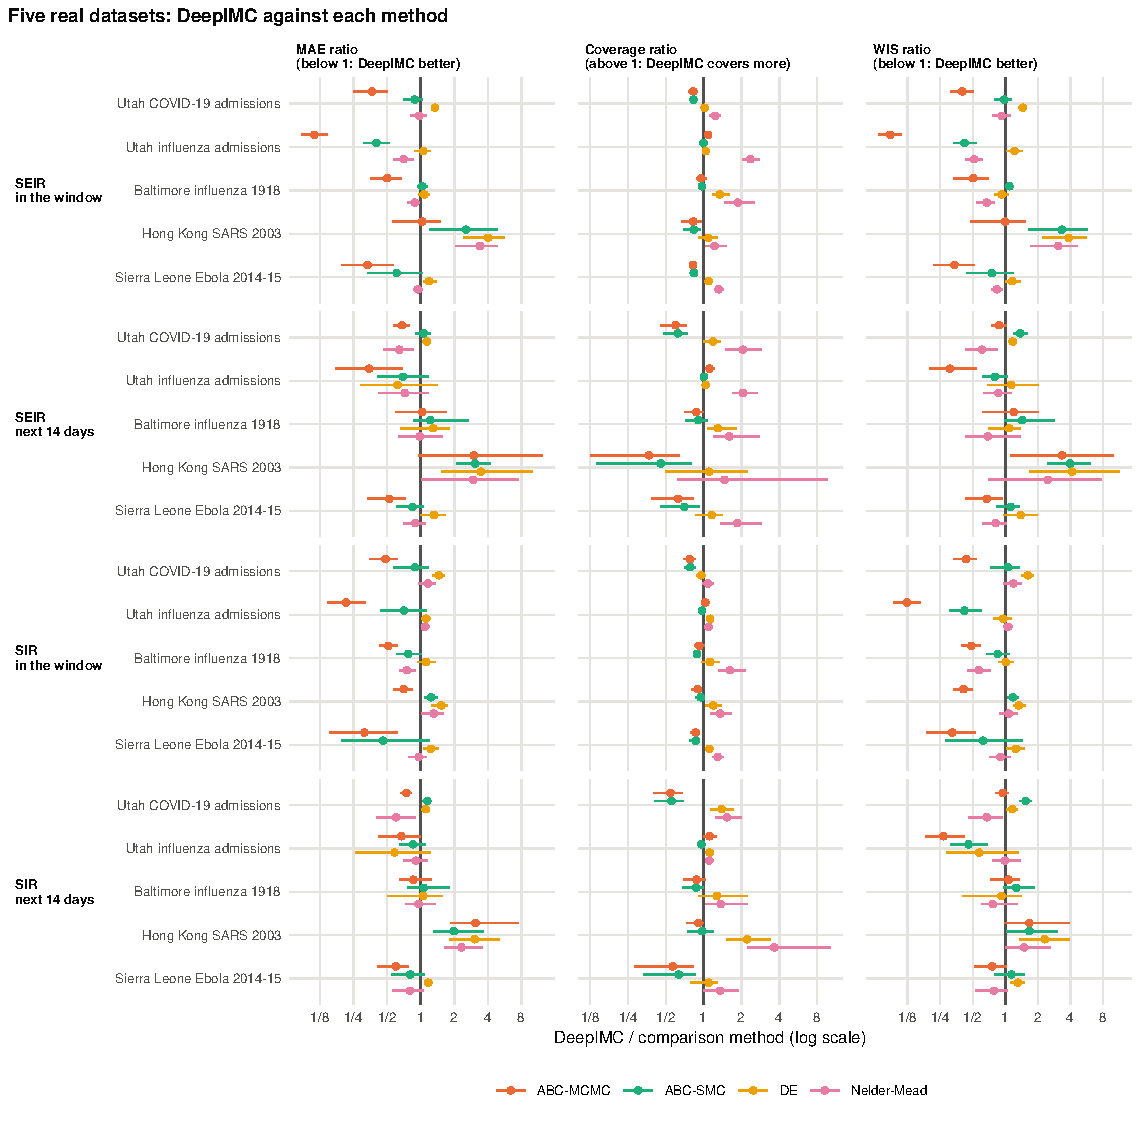
\includegraphics[width=\textwidth]{figures/ratios_real.pdf}
\caption{Real data: DeepIMC without weighting against each comparison method, as in Figure~\ref{fig:ratios-real}.}
\label{fig:ratios-real-auto}
\end{figure}

\begin{figure}[htbp]
\centering
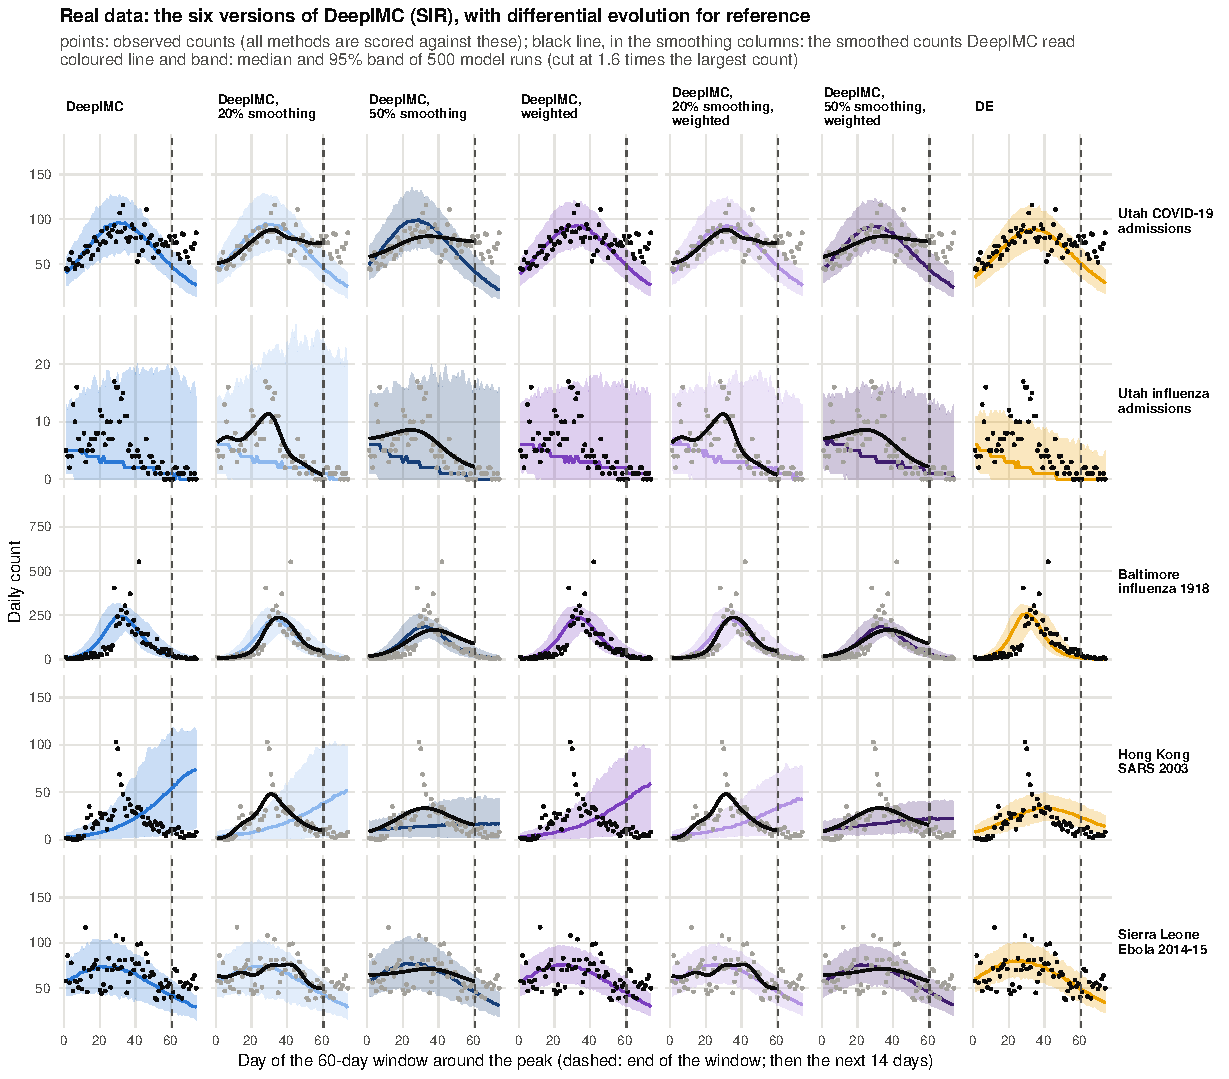
\includegraphics[width=\textwidth]{figures/real_examples_deepimc_sir.pdf}
\caption{Real data: the six versions of DeepIMC and differential evolution, SIR fits, as in
Figure~\ref{fig:real-examples-deepimc}.}
\label{fig:real-examples-deepimc-sir}
\end{figure}

\begin{figure}[htbp]
\centering
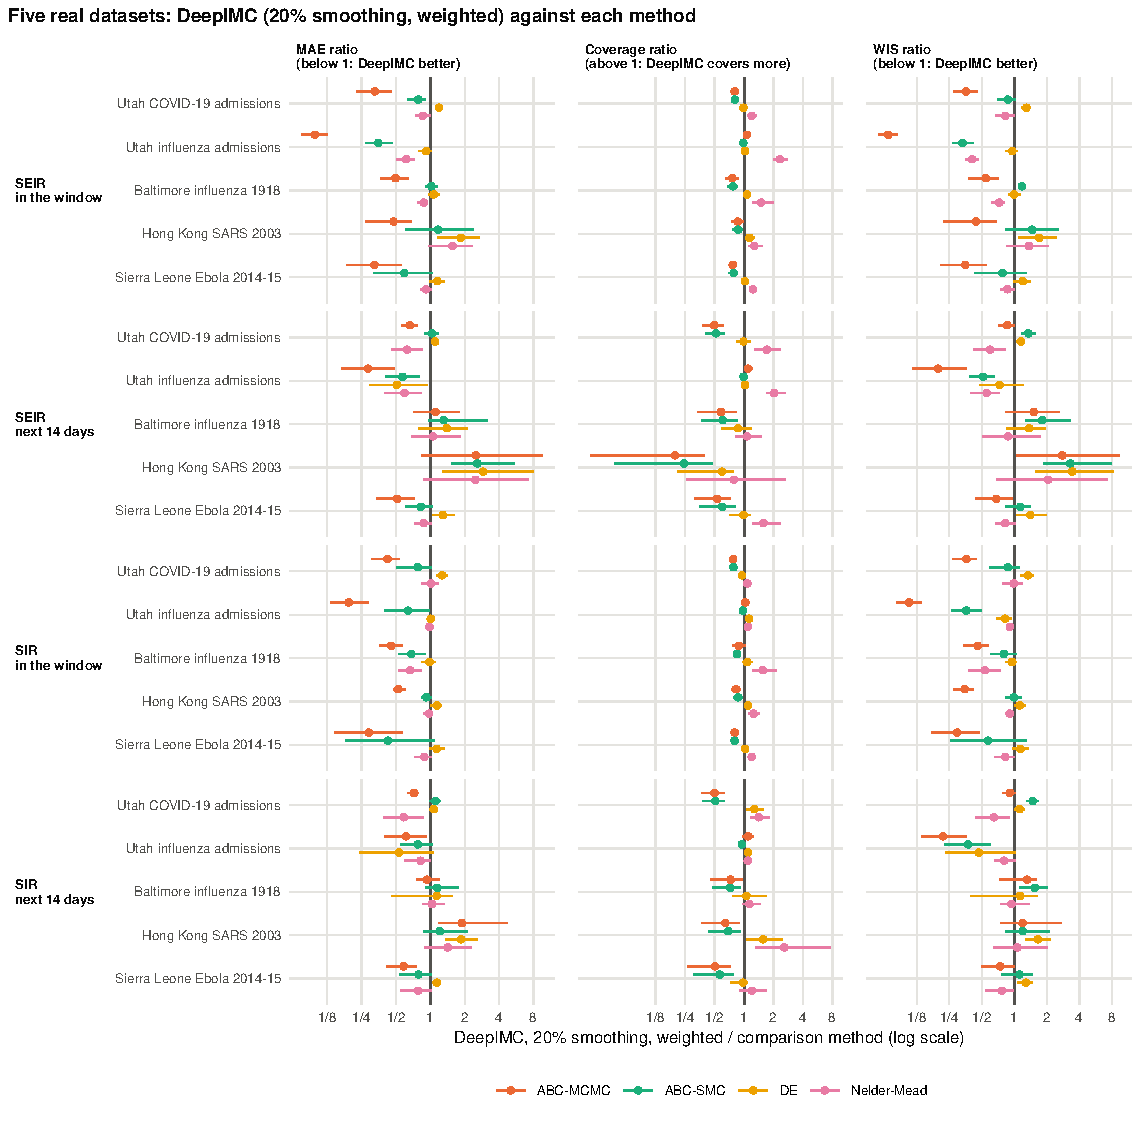
\includegraphics[width=\textwidth]{figures/ratios_real_weighted_k20.pdf}
\caption{Real data: the weighted DeepIMC reading counts smoothed by a Gaussian kernel of 20\% of the window length
against each comparison method, as in Figure~\ref{fig:ratios-real}.}
\label{fig:ratios-real-w20}
\end{figure}

\begin{figure}[htbp]
\centering
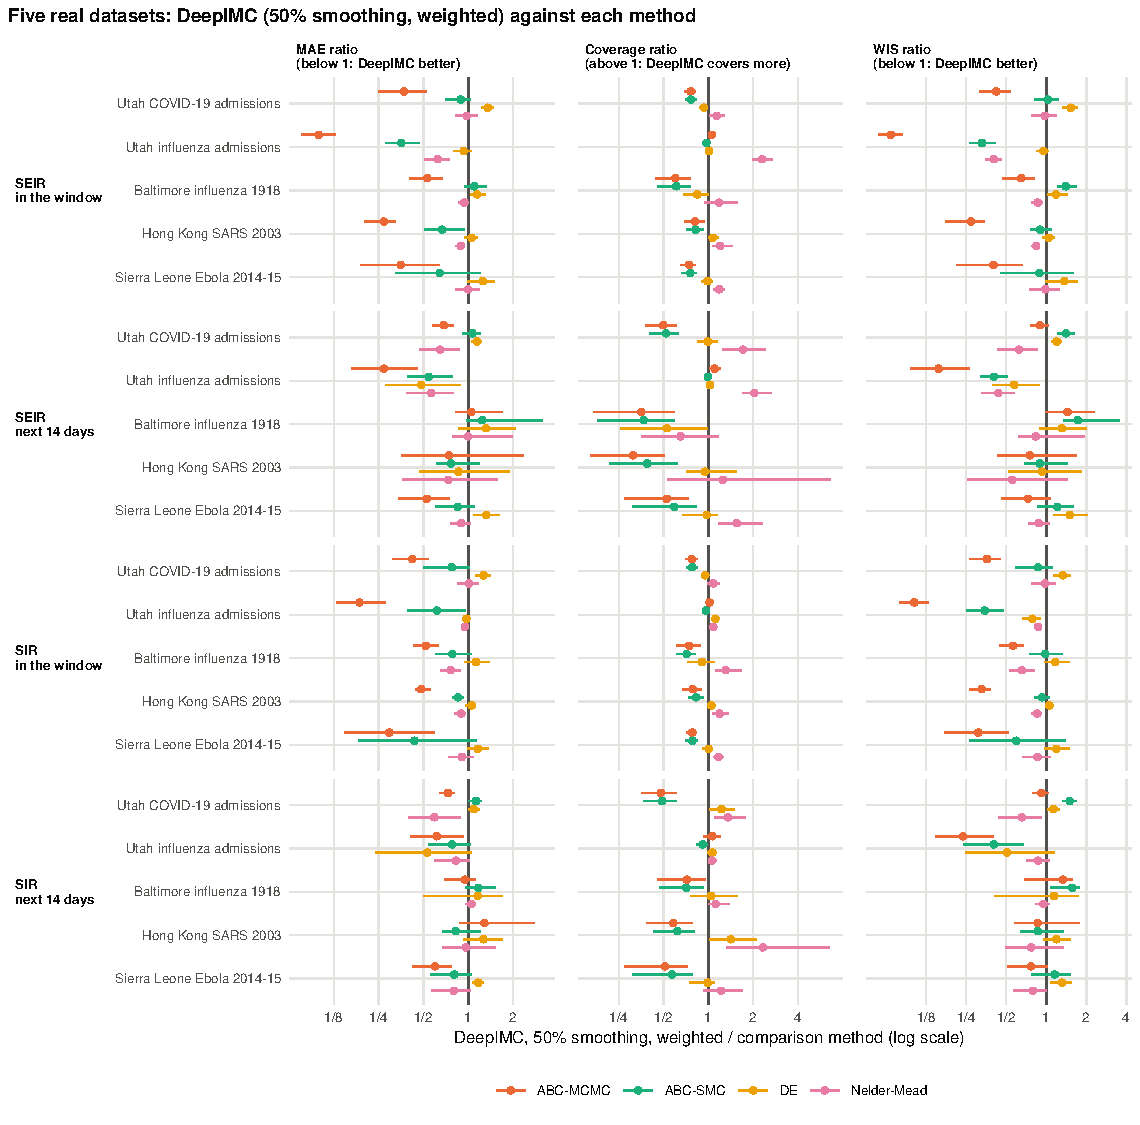
\includegraphics[width=\textwidth]{figures/ratios_real_weighted_k50.pdf}
\caption{Real data: the weighted DeepIMC reading counts smoothed by a Gaussian kernel of 50\% of the window length
against each comparison method, as in Figure~\ref{fig:ratios-real}.}
\label{fig:ratios-real-w50}
\end{figure}

\begin{table}[htbp]
\centering
\caption{Real data: cumulative counts since the first day of the window (an evaluation only): coverage (\%) of the
observed cumulative curve by the 95\% band, and its MAE as a percentage of the observed final count.}
\label{tab:real-cumulative}
\small
\resizebox{\textwidth}{!}{\begin{tabular}{llrrrrrrrrrr}
\toprule
Dataset & Model & DeepIMC & DeepIMC, 20\% & DeepIMC, 50\% & DeepIMC, weighted & DeepIMC, 20\%, weighted & DeepIMC, 50\%, weighted & ABC-MCMC & ABC-SMC & DE & Nelder--Mead \\
\midrule
\multicolumn{12}{l}{\textit{Coverage of the observed cumulative counts (\%)}} \\
Utah COVID-19 admissions (45) & SEIR & 88 & 87 & 80 & 89 & 87 & 82 & 100 & \textbf{94} & 73 & 45 \\
 & SIR & 83 & 82 & 80 & 84 & 83 & 83 & 100 & \textbf{91} & 75 & 58 \\
Utah influenza admissions (36) & SEIR & 99 & 99 & 97 & 100 & 99 & \textbf{97} & 63 & 91 & 91 & 18 \\
 & SIR & 100 & 100 & 100 & 100 & 100 & 100 & 100 & 100 & 87 & \textbf{94} \\
Baltimore influenza 1918 (12) & SEIR & 91 & 93 & 65 & 86 & 87 & 66 & \textbf{96} & 98 & 70 & 42 \\
 & SIR & 88 & 99 & 67 & 90 & \textbf{97} & 68 & 98 & 100 & 88 & 51 \\
Hong Kong SARS 2003 (12) & SEIR & 87 & \textbf{91} & 78 & 85 & 84 & 61 & 89 & 90 & 69 & 44 \\
 & SIR & 92 & 91 & 87 & 81 & 79 & 73 & 100 & \textbf{95} & 76 & 62 \\
Sierra Leone Ebola 2014-15 (18) & SEIR & 89 & 88 & 84 & 89 & 88 & 84 & 100 & \textbf{99} & 65 & 41 \\
 & SIR & \textbf{93} & 92 & 89 & 93 & 92 & 89 & 100 & 99 & 80 & 52 \\
Utah COVID-19 cases$^\dagger$ (48) & SEIR & 94 & 99 & 96 & 96 & 98 & 90 & \textbf{96} & 98 & 89 & 62 \\
 & SIR & 100 & 100 & 98 & 99 & 98 & \textbf{95} & 100 & 100 & 85 & 70 \\
\midrule
\multicolumn{12}{l}{\textit{MAE of the cumulative curve, \% of the final count}} \\
Utah COVID-19 admissions (45) & SEIR & 5.8 & 6.1 & 8.3 & 3.6 & 3.7 & 5.1 & 37.6 & 9.2 & \textbf{3.5} & 7.5 \\
 & SIR & 6.8 & 6.7 & 6.9 & 4.7 & \textbf{4.6} & 4.9 & 33.9 & 12.7 & 4.6 & 9.6 \\
Utah influenza admissions (36) & SEIR & 26.2 & 25.7 & 24.7 & 22.1 & 22.0 & 21.5 & 2,082.6 & 182.6 & \textbf{20.2} & 96.8 \\
 & SIR & 32.2 & 30.6 & 27.4 & 28.9 & 28.5 & \textbf{26.0} & 1,852.9 & 77.4 & 31.3 & 26.8 \\
Baltimore influenza 1918 (12) & SEIR & 8.5 & 8.2 & 12.3 & 7.3 & 5.4 & 7.5 & 62.2 & 11.4 & \textbf{5.4} & 13.5 \\
 & SIR & 12.6 & 7.7 & 9.1 & 7.7 & \textbf{5.6} & 7.7 & 28.8 & 9.3 & 14.6 & 13.3 \\
Hong Kong SARS 2003 (12) & SEIR & 44.3 & 19.5 & 14.8 & 38.3 & 14.9 & 12.4 & 381.3 & 26.9 & \textbf{8.1} & 18.9 \\
 & SIR & 22.1 & 22.3 & 19.6 & 15.2 & 15.6 & 12.9 & 138.4 & 18.7 & \textbf{11.4} & 15.6 \\
Sierra Leone Ebola 2014-15 (18) & SEIR & 8.6 & 8.0 & 7.1 & 6.1 & 6.0 & \textbf{5.5} & 105.2 & 18.4 & 7.5 & 12.4 \\
 & SIR & 10.0 & 9.6 & 8.8 & 6.1 & 6.1 & \textbf{5.8} & 94.2 & 19.4 & 5.9 & 11.0 \\
Utah COVID-19 cases$^\dagger$ (48) & SEIR & 27.3 & 18.7 & 14.5 & 16.2 & \textbf{9.6} & 10.2 & 1,963.2 & 53.8 & 10.3 & 21.9 \\
 & SIR & 25.5 & 24.1 & 20.8 & 12.6 & 13.4 & \textbf{12.3} & 310.3 & 26.2 & 34.5 & 34.8 \\
\bottomrule
\end{tabular}
}
\end{table}

\section{Supplementary results: six more outbreaks}\label{app:extra}

Of the five datasets, the SARS outbreak in Hong Kong is the one where DeepIMC fell furthest behind differential
evolution. To learn whether this is a property of SARS, of outbreaks that spread through large clusters of cases, or
of the Hong Kong data, we added six outbreaks counted by date of symptom onset (Table~\ref{tab:datasets-extra},
Figure~\ref{fig:extra-series}). SARS in Canada, MERS in South Korea and smallpox in Kosovo spread largely through
clusters in hospitals \autocite{cowling2015preliminary,fenner1988smallpox}; influenza in a school, measles in a
village and Ebola in Kikwit are well-studied small outbreaks. Their counts are small, with peaks of 9 to 20 cases a
day, so their scores are small too and should be compared between methods rather than with those of the five
datasets. Everything else (the networks, settings, windows, effective population and scores) is as for the five
datasets, and these outbreaks are not part of the averages over the five datasets.

\begin{table}[htbp]
\centering
\caption{The six more outbreaks: what each counts, its period, number of cases and source, the windows per model,
and the known values for each disease (SEIR latent period incub in days and recovery rate; SIR recovery rate), set
as in Section~\ref{sec:eval-real}.}
\label{tab:datasets-extra}
\small
\begin{tabular}{>{\raggedright\arraybackslash}p{2.6cm} >{\raggedright\arraybackslash}p{3.4cm} >{\raggedright\arraybackslash}p{3.4cm} >{\raggedleft\arraybackslash}p{1.2cm} >{\raggedright\arraybackslash}p{3.2cm}}
\toprule
Outbreak & What is counted (by date of) & Period, cases and source & Windows per model & Known values (SEIR; SIR) \\
\midrule
Canada SARS 2003 & SARS cases, most of them in Toronto (symptom onset) & 23 Feb--12 Jun 2003, 250 cases; Health Canada \autocite{devries2006course,jombart2020outbreaks} & 12 & as Hong Kong SARS \\
South Korea MERS 2015 & MERS cases with a known onset date (symptom onset) & 11 May--15 Jun 2015, 135 cases; ECDC line list \autocite{jombart2020outbreaks} & 6 & incub 6.7, $p_{recov}$ 0.169; $p_{recov}$ 0.079 \autocite{cowling2015preliminary} \\
Kosovo smallpox 1972 & smallpox cases (symptom onset) & 57 days, 124 cases \autocite{fenner1988smallpox,cori2013new} & 6 & incub 12, $p_{recov}$ 0.096; $p_{recov}$ 0.071 \autocite{fenner1988smallpox,cori2013new} \\
Pennsylvania influenza 2009 & acute respiratory illness in the children of a school (symptom onset) & 27 Apr--28 May 2009, 129 cases \autocite{cauchemez2011role,cori2013new} & 6 & as Utah influenza \\
Hagelloch measles 1861 & measles in the children of a village (onset of the first symptoms) & 30 Oct 1861--24 Jan 1862, 188 cases \autocite{pfeilsticker1863,neal2004statistical} & 9 & incub 12.5, $p_{recov}$ 0.25; $p_{recov}$ 0.071 \autocite{lessler2009incubation,cori2013new} \\
Kikwit Ebola 1995 & Ebola cases (symptom onset) & 6 Jan--16 Jul 1995, 292 cases \autocite{khan1999reemergence} & 18 & as Sierra Leone Ebola \\
\bottomrule
\end{tabular}
\end{table}

\paragraph{Fit to the data.} Table~\ref{tab:real-extra} gives the coverage and the WIS for each outbreak and model,
with Hong Kong for comparison, and Figure~\ref{fig:extra-examples} shows the fits around the peak. In the window, a
version of DeepIMC had the lowest WIS on 8 of the 12 combinations of outbreak and model, and the weighted DeepIMC on
the raw counts was closer to the data than every comparison method on 6 of them; differential evolution or ABC-SMC
was closest on MERS under the SEIR model, smallpox under the SIR model and measles. Over the 114 windows the weighted
DeepIMC's bands covered 91\% of the observed days, against 89\% for differential evolution and 99\% for ABC-SMC,
and its WIS was 1.20, against 1.39 and 1.79. In the next 14 days its WIS (3.6) was close to that of ABC-SMC (3.8)
and below that of differential evolution (6.3). Unlike on the five datasets, heavy smoothing helped here: with a
kernel of 50\% of the window and the weighting, DeepIMC's WIS was 1.12 in the window and 1.9 in the next 14 days,
the lowest of all methods (with a kernel of 20\%, 1.17 and 2.8), probably because with so few cases the day-to-day noise is large compared with the
counts of most training epidemics.

\paragraph{Noise and the fit check.} Table~\ref{tab:real-extra-check} shows how noisy each outbreak's counts are and
how often DeepIMC's draws reproduce its windows. The Hong Kong counts were the noisiest: their dispersion index was
4.2, against 0.6 to 2.4 for the six outbreaks and about 0.9 for the agent-based model's own curves. The fit check
flagged 62\% of the Hong Kong windows and 23\% of those of the six outbreaks: none for SARS in Canada, 8\% for MERS
and influenza, and 28 to 50\% for Ebola, measles and smallpox. A flag says only that no draw reproduces the window
within twice the Poisson noise; half of the smallpox windows were flagged, yet there the weighted DeepIMC was as
close to the data as differential evolution (a median WIS ratio of 0.94). Over the windows of each outbreak, the
median WIS ratio of the weighted DeepIMC to differential evolution was 0.93 to 1.08, and to ABC-SMC 0.68 to 0.94.
For Hong Kong it was 1.05: in a typical Hong Kong window DeepIMC was about as close to the data as differential
evolution, and its mean WIS is dominated by the windows that contain the jump.

\paragraph{Measles in Hagelloch.} Where DeepIMC fell behind on these outbreaks, as on the 60-day measles window of
Figure~\ref{fig:extra-examples}, it continued the growth of the window while the outbreak ended. The 188 cases
were almost all the children of the village \autocite{neal2004statistical}: the outbreak stopped when the
susceptible children ran out, which an effective population of 10,000 cannot reproduce. In the 14 days after the
measles windows, the weighted DeepIMC's WIS was 12.3 under the SEIR model, against 3.0 for differential evolution.

\paragraph{The Hong Kong jump.} Table~\ref{tab:hk-jump} splits the 24 Hong Kong windows (both models) by their
position relative to the jump from 31 to 103 cases between days 37 and 38 (Figure~\ref{fig:extra-series}). The four
windows that end before the jump and the six that start after it were fitted as closely by the weighted DeepIMC as
by any comparison method (WIS 1.42 and 0.67, against 1.57 and 0.77 for differential evolution), and the fit check
flagged one of these ten windows. The 14 windows that contain the jump were all flagged; on them the weighted
DeepIMC's WIS was 20.5, against 8.9 for differential evolution and 10.0 for ABC-SMC. DeepIMC read the jump as the
start of fast growth and, having learned from epidemics with constant parameters, continued it
(Figure~\ref{fig:extra-examples}, first row), while the methods that fit the whole window found a slower epidemic
that passes through the middle of the counts. A kernel of 50\% of the window spreads the jump; with the weighting it
brought DeepIMC's WIS on these windows to 9.4, close to that of differential evolution. A cluster in which hundreds
of people were infected at the same time \autocite{yu2004evidence} is outside what a homogeneous agent-based model
with constant transmission describes. That cluster, and not SARS or real data in general, is why Hong Kong is the
dataset where DeepIMC fell furthest behind.

\begin{sidewaystable}
\centering
\caption{Six more outbreaks, with Hong Kong SARS for comparison: coverage (\%) of the observed counts in the window
by the 95\% band, and WIS in the window and in the next 14 days (where the outbreak continues), mean over the
windows of each outbreak (number of windows per model in brackets). DeepIMC is shown on the raw counts, weighted by
the data, and weighted with the counts smoothed by a Gaussian kernel of 20\% or 50\% of the window length; every
version is scored against the raw counts. Bold: coverage closest to 95\% and lowest WIS.}
\label{tab:real-extra}
\footnotesize
\resizebox{\textheight}{!}{\begin{tabular}{llrrrrrrrr}
\toprule
Dataset & Model & DeepIMC & DeepIMC, weighted & DeepIMC, 20\%, weighted & DeepIMC, 50\%, weighted & ABC-MCMC & ABC-SMC & DE & Nelder--Mead \\
\midrule
\multicolumn{10}{l}{\textit{Coverage of the observed counts in the window (\%)}} \\
Hong Kong SARS 2003 (12) & SEIR & 77 & 78 & 80 & 75 & \textbf{93} & 92 & 70 & 63 \\
 & SIR & 90 & 83 & 83 & 79 & 100 & \textbf{95} & 75 & 66 \\
Canada SARS 2003 (12) & SEIR & 98 & 96 & 96 & \textbf{95} & 98 & 100 & 93 & 79 \\
 & SIR & 98 & 96 & 96 & \textbf{95} & 100 & 100 & 91 & 86 \\
South Korea MERS 2015 (6) & SEIR & \textbf{95} & 87 & 88 & 90 & 99 & 100 & 88 & 76 \\
 & SIR & 84 & 84 & 86 & 87 & 100 & \textbf{99} & 84 & 80 \\
Kosovo smallpox 1972 (6) & SEIR & 88 & 86 & 86 & 85 & \textbf{94} & 100 & 83 & 73 \\
 & SIR & 98 & 90 & 88 & 88 & 100 & \textbf{96} & 78 & 83 \\
Pennsylvania influenza 2009 (6) & SEIR & 100 & 94 & 90 & 89 & \textbf{96} & 99 & 86 & 57 \\
 & SIR & 98 & 91 & 91 & \textbf{92} & 100 & 100 & 87 & 91 \\
Hagelloch measles 1861 (9) & SEIR & 86 & 83 & 86 & 88 & 99 & \textbf{97} & 90 & 73 \\
 & SIR & 91 & 89 & 90 & 88 & 100 & \textbf{96} & 85 & 81 \\
Kikwit Ebola 1995 (18) & SEIR & 99 & 95 & \textbf{95} & 93 & 94 & 100 & 93 & 81 \\
 & SIR & 99 & 92 & 93 & \textbf{94} & 100 & 99 & 91 & 91 \\
\midrule
\multicolumn{10}{l}{\textit{WIS in the window}} \\
Hong Kong SARS 2003 (12) & SEIR & 21.98 & 18.44 & 9.73 & 5.99 & 22.06 & 6.64 & \textbf{5.73} & 7.13 \\
 & SIR & 7.32 & 6.26 & 6.18 & 5.82 & 17.83 & 6.26 & \textbf{5.51} & 6.81 \\
Canada SARS 2003 (12) & SEIR & 0.92 & \textbf{0.86} & 0.87 & 0.88 & 13.69 & 1.33 & 0.88 & 1.35 \\
 & SIR & 1.07 & 0.89 & 0.89 & \textbf{0.88} & 8.27 & 1.08 & 1.29 & 1.07 \\
South Korea MERS 2015 (6) & SEIR & 1.49 & 1.46 & 1.43 & 1.44 & 21.48 & 4.24 & \textbf{1.36} & 2.08 \\
 & SIR & 2.98 & 1.85 & 1.73 & \textbf{1.51} & 13.36 & 1.99 & 1.72 & 2.23 \\
Kosovo smallpox 1972 (6) & SEIR & 1.52 & 1.51 & \textbf{1.45} & 1.46 & 13.48 & 1.93 & 1.50 & 2.00 \\
 & SIR & 2.32 & 1.44 & 1.45 & 1.43 & 19.90 & \textbf{1.21} & 1.78 & 1.81 \\
Pennsylvania influenza 2009 (6) & SEIR & 1.93 & \textbf{1.48} & 1.51 & 1.54 & 17.01 & 1.68 & 1.86 & 3.31 \\
 & SIR & 1.89 & 1.68 & 1.66 & \textbf{1.62} & 5.20 & 2.03 & 1.72 & 1.74 \\
Hagelloch measles 1861 (9) & SEIR & 2.39 & 1.96 & 1.48 & 1.36 & 13.14 & 1.44 & \textbf{1.33} & 1.93 \\
 & SIR & 1.92 & 1.39 & 1.36 & 1.33 & 10.13 & \textbf{1.28} & 1.46 & 1.84 \\
Kikwit Ebola 1995 (18) & SEIR & 1.67 & \textbf{0.77} & 0.93 & 0.79 & 16.09 & 1.43 & 0.83 & 1.05 \\
 & SIR & 1.96 & 0.86 & 0.82 & \textbf{0.80} & 9.33 & 2.48 & 1.85 & 0.91 \\
\midrule
\multicolumn{10}{l}{\textit{WIS in the next 14 days}} \\
Hong Kong SARS 2003 (12) & SEIR & 57.07 & 52.58 & 47.43 & \textbf{12.84} & 17.07 & 14.37 & 13.79 & 23.14 \\
 & SIR & 19.71 & 15.94 & 14.09 & 10.19 & 11.84 & 11.80 & \textbf{8.55} & 13.22 \\
Canada SARS 2003 (12) & SEIR & 2.61 & 2.38 & 2.25 & 1.57 & 12.55 & 2.41 & \textbf{1.33} & 4.75 \\
 & SIR & \textbf{1.33} & 1.33 & 1.44 & 1.38 & 6.94 & 2.90 & 7.66 & 1.42 \\
South Korea MERS 2015 (6) & SEIR & 3.58 & 3.62 & 3.22 & \textbf{2.87} & 25.30 & 9.20 & 3.99 & 5.44 \\
 & SIR & 3.75 & 2.65 & \textbf{2.61} & 2.86 & 18.82 & 5.96 & 8.81 & 9.25 \\
Kosovo smallpox 1972 (6) & SEIR & 4.19 & 3.66 & 2.70 & 2.47 & 16.11 & 2.85 & \textbf{2.31} & 4.64 \\
 & SIR & 4.56 & 2.92 & 2.42 & 2.46 & 16.55 & \textbf{1.90} & 8.21 & 10.04 \\
Pennsylvania influenza 2009 (6) & SEIR & 17.11 & 14.78 & 11.35 & 6.05 & 14.20 & 7.48 & 18.75 & \textbf{3.01} \\
 & SIR & 1.82 & 1.49 & 1.76 & \textbf{1.49} & 10.07 & 7.50 & 5.63 & 2.66 \\
Hagelloch measles 1861 (9) & SEIR & 18.39 & 12.30 & 5.03 & \textbf{2.00} & 16.03 & 3.49 & 3.02 & 5.30 \\
 & SIR & 2.50 & 2.15 & 2.09 & \textbf{1.87} & 13.89 & 3.00 & 2.50 & 5.48 \\
Kikwit Ebola 1995 (18) & SEIR & 2.49 & 1.26 & 2.62 & \textbf{0.84} & 11.95 & 2.22 & 1.70 & 1.83 \\
 & SIR & 1.89 & 1.25 & \textbf{0.77} & 0.90 & 8.10 & 3.17 & 12.82 & 3.45 \\
\bottomrule
\end{tabular}
}
\end{sidewaystable}

\begin{table}[htbp]
\centering
\caption{Six more outbreaks, with Hong Kong SARS for comparison: windows (both models); largest daily count;
dispersion index of the counts (variance around a centred 7-day mean divided by that mean, median over the windows
of 30 days or more; about 0.9 for the agent-based model's own curves); percentage of windows that no draw of DeepIMC
reproduces within twice the Poisson noise ($d_{\min} > 1$, Section~\ref{sec:weighting}); and the weighted DeepIMC's
WIS divided by that of differential evolution and of ABC-SMC (median over the windows).}
\label{tab:real-extra-check}
\small
\begin{tabular}{lrrrrrr}
\toprule
 & Windows & Peak & Dispersion & Not repro- & \multicolumn{2}{c}{Weighted DeepIMC WIS /} \\
\cmidrule(lr){6-7}
Outbreak &  & count & index & duced (\%) & DE WIS & ABC-SMC WIS \\
\midrule
Hong Kong SARS 2003 & 24 & 103 & 4.19 & 62 & 1.05 & 0.88 \\
\midrule
Canada SARS 2003 & 24 & 9 & 0.57 & 0 & 0.93 & 0.87 \\
South Korea MERS 2015 & 12 & 16 & 1.01 & 8 & 0.94 & 0.92 \\
Kosovo smallpox 1972 & 12 & 20 & 2.38 & 50 & 0.94 & 0.82 \\
Pennsylvania influenza 2009 & 12 & 13 & 0.58 & 8 & 0.94 & 0.94 \\
Hagelloch measles 1861 & 18 & 20 & 1.59 & 44 & 1.08 & 0.93 \\
Kikwit Ebola 1995 & 36 & 15 & 1.09 & 28 & 0.95 & 0.68 \\
\midrule
All six & 114 &  & 1.06 & 23 & 0.95 & 0.88 \\
\bottomrule
\end{tabular}

\end{table}

\begin{table}[htbp]
\centering
\caption{Hong Kong SARS: the 24 windows (both models) split by the jump of the counts from 31 to 103 between days
37 and 38: windows that end before it, contain it, or start after it. Percentage of windows flagged by the fit
check, and mean WIS in the window. Bold: lowest WIS.}
\label{tab:hk-jump}
\small
\begin{tabular}{lrrr}
\toprule
 & \multicolumn{3}{c}{Windows that \ldots\ the jump} \\
\cmidrule(lr){2-4}
 & end before & contain & start after \\
\midrule
Windows (both models) & 4 & 14 & 6 \\
Not reproduced (\%) & 25 & 100 & 0 \\
\midrule
\multicolumn{4}{l}{\textit{WIS in the window}} \\
DeepIMC & 1.88 & 24.16 & 0.96 \\
DeepIMC, weighted & 1.42 & 20.47 & \textbf{0.67} \\
DeepIMC, 20\%, weighted & 1.40 & 12.94 & 0.68 \\
DeepIMC, 50\%, weighted & \textbf{1.33} & 9.40 & 0.80 \\
ABC-MCMC & 13.30 & 26.32 & 9.49 \\
ABC-SMC & 2.00 & 10.04 & 1.06 \\
DE & 1.57 & \textbf{8.86} & 0.77 \\
Nelder--Mead & 2.48 & 10.86 & 0.89 \\
\bottomrule
\end{tabular}

\end{table}

\begin{figure}[htbp]
\centering
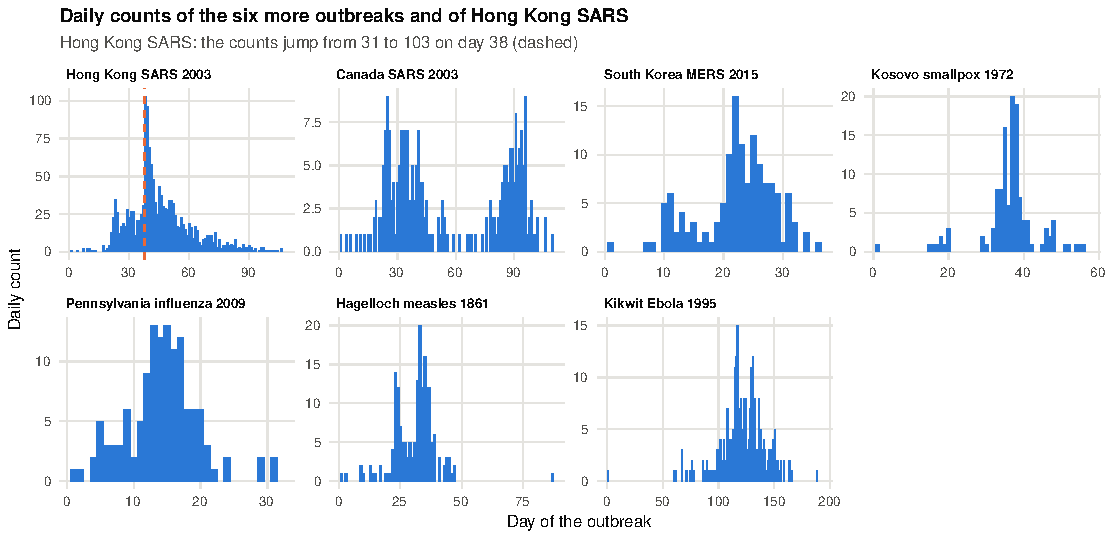
\includegraphics[width=\textwidth]{figures/real_extra_series.pdf}
\caption{Daily counts of the six more outbreaks and of the Hong Kong SARS outbreak. Dashed: the day on which the
Hong Kong counts jump from 31 to 103.}
\label{fig:extra-series}
\end{figure}

\begin{figure}[htbp]
\centering
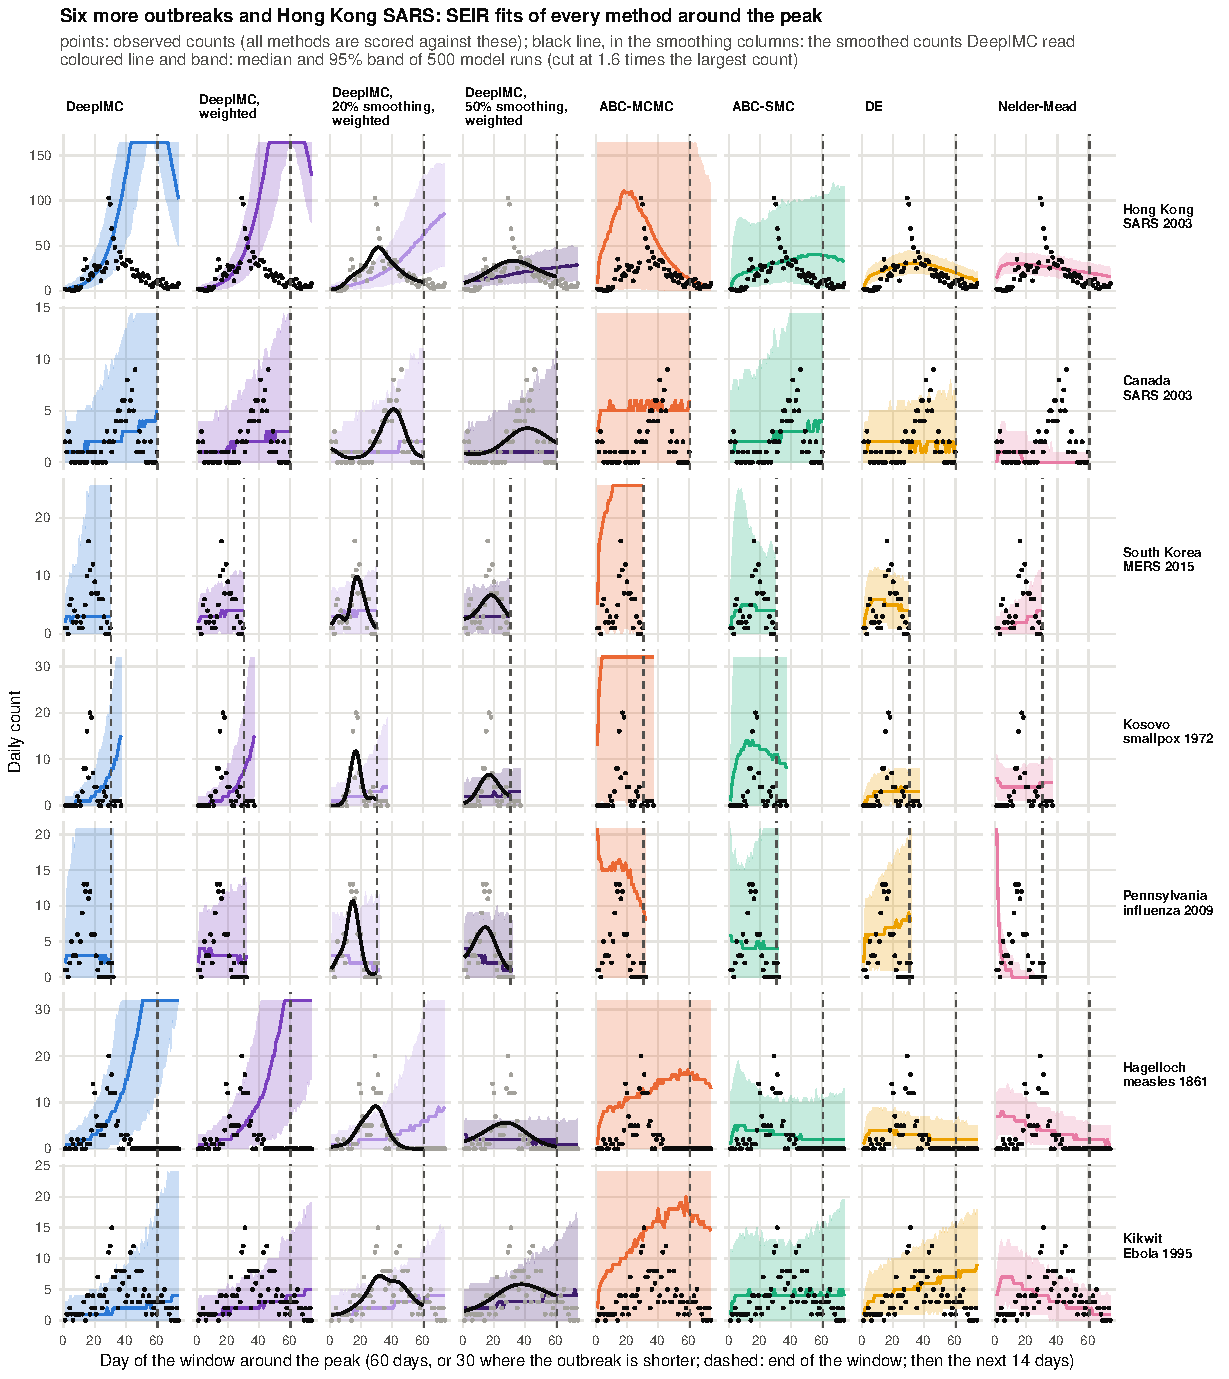
\includegraphics[width=\textwidth]{figures/real_extra_examples.pdf}
\caption{Six more outbreaks and Hong Kong SARS: SEIR fits of every method to the window in the middle of each
outbreak (60 days, or 30 days for the shorter MERS, smallpox and influenza outbreaks), with the following days
(after the dashed line; fewer than 14 where the outbreak ends). Points: observed counts, against which every method
is scored; black line: the smoothed counts DeepIMC read in the smoothing columns; coloured lines and bands: median and
95\% band of 500 model runs (cut at 1.6 times the largest observed count).}
\label{fig:extra-examples}
\end{figure}

\section{Supplementary results: sensitivity of the comparison methods}\label{app:sensitivity}

\paragraph{Differential evolution with a new seed for every model run.} In the paper, differential evolution
runs every candidate with the same random seed, so that a candidate always receives the same fit; this is an
expert's choice. A user who simply calls the stochastic model draws a new seed for every run. On 1,000 windows
of the simulated test of windows of 15 to 365 days and on the real windows, the two versions gave almost the same
results (Table~\ref{tab:de-typical}): $R_0$ MAE 0.73 and 0.71 (SEIR) and 0.55 and 0.53 (SIR), and the same
coverage and MAE on the real data. Differential evolution's close fit to the observed curve therefore does not
depend on the fixed seed; it comes from fitting each window directly.

\begin{table}[htbp]
\centering
\caption{Differential evolution as set up in the paper (one fixed random seed for every candidate) and as a
typical user would run it (a new random seed for every model run), with DeepIMC for reference: 1,000 windows of
the simulated test of windows of 15 to 365 days (500 per model), and the real windows.}
\label{tab:de-typical}
\small
\resizebox{\textwidth}{!}{\begin{tabular}{llrrrrrr}
\toprule
 &  & \multicolumn{4}{c}{1,000 simulated windows} & \multicolumn{2}{c}{Real data (window)} \\
\cmidrule(lr){3-6}\cmidrule(lr){7-8}
Model & Method & $R_0$ MAE & State error & MAE, new inf. & Cov., infectious (\%) & Cov. (\%) & MAE \\
\midrule
SEIR & DeepIMC & 0.20 & 1.5 & 4.8 & 98.2 & -- & -- \\
 & DE & 0.73 & 4.6 & 4.7 & 77.4 & 80.9 & 9.4 \\
 & DE, new seed per run & 0.71 & 4.6 & 4.7 & 76.4 & 81.0 & 9.3 \\
\midrule
SIR & DeepIMC & 0.19 & 2.6 & 6.5 & 98.3 & -- & -- \\
 & DE & 0.55 & 6.1 & 6.0 & 71.5 & 79.2 & 10.0 \\
 & DE, new seed per run & 0.53 & 5.8 & 6.0 & 73.1 & 79.2 & 10.7 \\
\bottomrule
\end{tabular}
}
\end{table}

\paragraph{ABC-SMC with more generations.} ABC-SMC is used with six generations, the default of the
implementation. With twelve generations (Table~\ref{tab:smc-generations}) its $R_0$ error fell from 0.65 to 0.51
(SEIR) and from 0.47 to 0.34 (SIR) and its ranges narrowed, still well behind DeepIMC, but each window needed 7 to 9
times as many model runs, and 10 of the 60 SEIR and 7 of the 60 SIR windows exhausted a budget of 200,000 runs.
With twenty generations almost every window exhausted the budget (all but 4 SEIR and 8 SIR windows): the tolerance
became smaller than the randomness of the agent-based model allows. Six generations are therefore a fair setting for the comparison.

\begin{table}[htbp]
\centering
\caption{ABC-SMC with 6 (as in the paper), 12 or 20 generations on 120 windows of the simulated test of windows of
15 to 365 days (60 per model; 20 early, middle and late), with a budget of 200,000 model runs: windows finished,
$R_0$ MAE, coverage and width of the 95\% range, model runs and seconds per window (means over the finished
windows; ``--'': fewer than 10 finished).}
\label{tab:smc-generations}
\small
\resizebox{\textwidth}{!}{\begin{tabular}{llrrrrrr}
\toprule
Model & Generations & Finished & $R_0$ MAE & Range has true (\%) & Range width & Model runs & Seconds \\
\midrule
SEIR & 6 & 60 of 60 & 0.65 & 92 & 3.07 & 5,127 & 270 \\
 & 12 & 50 of 60 & 0.51 & 96 & 2.51 & 47,386 & 2,495 \\
 & 20 & 4 of 60 & -- & -- & -- & 85,522 & 1,834 \\
\midrule
SIR & 6 & 60 of 60 & 0.47 & 100 & 2.60 & 4,207 & 97 \\
 & 12 & 53 of 60 & 0.34 & 100 & 1.68 & 28,956 & 697 \\
 & 20 & 8 of 60 & -- & -- & -- & 82,306 & 1,042 \\
\bottomrule
\end{tabular}
}
\end{table}

\section{Supplementary results: predicting with the renewal equation}\label{sec:res-renewal}

Running the agent-based model 500 times for every band is the slowest part of a prediction. The renewal
equation is a deterministic shortcut that gives the model's average curve.

\paragraph{Renewal A.} Started from DeepIMC's estimated state, the renewal equation gave almost the same
curves of new infections as 500 runs of the agent-based model (Table~\ref{tab:renewal}): in the window, a
coverage of 97.5\% against 98.1\% and an MAE of 5.0 against 4.8 for SEIR (96.2\% and 7.8 against 98.9\% and
6.1 for SIR), and the same coverage and MAE over the next 14 days. Its bands for the number currently infectious were narrower than those of the model, because
they contain only Poisson noise around the average and none of the randomness of the epidemic itself, and
covered 86--89\% of the days instead of 98--99\%. On one CPU core, it took 0.20 seconds per SEIR window
instead of 38 seconds for 500 model runs (Table~\ref{tab:timing}).

\paragraph{Renewal B.} Fitting the starting state with the renewal equation did not help. The fitted state was
less accurate than DeepIMC's (2.0 against 1.4 percentage points for SEIR, 2.7 against 2.2 for SIR). The fitted
curve was slightly closer to the observed new infections (MAE 4.4 against 4.8 for SEIR), but from the curve
alone the renewal fit cannot separate exposed from infectious people, and its bands covered the true number of
infectious people on only 39--47\% of the days. Renewal B was also much slower than renewal A, because it fits
the state at 30 values of $R_0$.

\begin{table}[htbp]
\centering
\caption{From DeepIMC's estimates to curves on the simulated test windows: 500 runs of the agent-based
model, or the renewal equation started from DeepIMC's state (A) or from a state fitted by the renewal
equation (B). Starting-state error (percentage points); coverage (\%) of the true curves and MAE of the
median curve; seconds per window during the evaluation, on shared computers (Table~\ref{tab:timing}
compares the times on one dedicated core).}
\label{tab:renewal}
\small
\resizebox{\textwidth}{!}{\begin{tabular}{llrrrrrrrr}
\toprule
 &  & State & \multicolumn{2}{c}{New infections} & \multicolumn{2}{c}{Currently infectious} & \multicolumn{2}{c}{Next 14 days} & Seconds \\
\cmidrule(lr){4-5}\cmidrule(lr){6-7}\cmidrule(lr){8-9}
Model & Curves from & error & Cov. & MAE & Cov. & MAE & Cov. & MAE & per window \\
\midrule
SEIR & model, 500 runs & 1.5 & 98.1 & 4.8 & 98.4 & 17.9 & 98.8 & 1.8 & 21.0 \\
 & renewal A & 1.5 & 97.5 & 5.0 & 89.2 & 19.0 & 98.3 & 1.8 & 0.88 \\
 & renewal B & 2.1 & 96.6 & 4.3 & 38.5 & 24.1 & 97.2 & 1.7 & 19.6 \\
\midrule
SIR & model, 500 runs & 2.7 & 98.8 & 6.2 & 98.7 & 35.1 & 99.1 & 1.0 & 7.8 \\
 & renewal A & 2.7 & 96.5 & 7.7 & 88.5 & 41.0 & 98.2 & 1.0 & 0.50 \\
 & renewal B & 3.2 & 95.5 & 5.2 & 48.8 & 41.4 & 97.6 & 0.9 & 5.10 \\
\bottomrule
\end{tabular}
}
\end{table}

\section{Renewal equation}\label{app:renewal}

With $\beta = R_0\, p_{recov}$ (the daily transmission rate $p_{tran}\, c_{rate}$), $\sigma = 1/\text{incub}$
and $\gamma = p_{recov}$, starting from $S_0$, $E_0$, $I_0$ (the estimated numbers on the first day of the
window), we compute for $t = 1, 2, \dots$
\begin{align*}
\text{new infections}_t &= S_{t-1}\left(1 - e^{-\beta I_{t-1}/N}\right),\\
C_t &= \sigma E_{t-1} \ \text{(SEIR)}, \qquad C_t = \text{new infections}_t \ \text{(SIR)},\\
E_t &= E_{t-1} + \text{new infections}_t - C_t \ \text{(SEIR)},\\
I_t &= I_{t-1} + C_t - \gamma I_{t-1}, \qquad S_t = S_{t-1} - \text{new infections}_t .
\end{align*}
Because the latent and infectious periods are geometric, this recursion equals the renewal equation
(\ref{eq:renewal}) with generation interval $g_k = \sum_{u+s=k} \sigma(1-\sigma)^{u-1}\, \gamma(1-\gamma)^{s-1}$
for SEIR and $g_k = \gamma(1-\gamma)^{k-1}$ for SIR, with the people already exposed or infectious at the
start of the window as its initial condition.

\end{document}
